\chapter{Angular fit strategy}

In this chapter is described the fitting technique applied to extract the angular observables.
There are physical limits to the values of the parameters of interests:
$A_{\rm FB}^h$ is limited in the [-0.5,0.5] interval and for the $f_{\rm L}$ and 
$A_{\rm FB}^\ell$ parameters the physical region, given by $|A_{\rm FB}^\ell| < 3/4(f_L-1)$,
is the triangle shown in Fig.~\ref{fig:pdfscan}.
If the minimum is close to the border minuit does not always converge. For this reason
a "brute force" fitting technique is applied. For this purpose fit parameters are
divided into two categories: parameters of interest (PoIs), $A_{\rm FB}^\ell$,
$A_{\rm FB}^h$ and $f_{\rm L}$ and all other parameters referred to as nuisances.
The Log-Likelihood, $log\mathcal{L}$, of the fit model with respect of data is calculated.
The full PoIs allowed area is scanned looking for the minimum of the Log-Likelihood.
A first coarse scan finds a candidate minimum and then the procedure is reiterated two
more times in finer intervals around it. For each point all the niusances are fitted
using a maximum likelihood fit. The fit is therefore constrained inside the physical
region, if the best log-likelihood is found to be outside it, the point at the boundary
is chosen as the best fit. %More details are given in Sec.~\ref{sec:FeldmanCousin}.

\section{Feldman-cousins plug-in method}
\label{sec:FeldmanCousins}
Feldman-Cousins plug-in method~\cite{Karbach:2011uz} is a unified method to calculate confidence
intervals and upper/lower limits, based on simulated experiments. 
This approach is used t calculate uncertainties since physical boundaries of the parameter space
could result in a wrong estimation of the uncertainties if the measured value is close to the border.
The method has the advantage of having a well defined frequentist coverage.

%One defines two classes of parameters: Parameters of Interest (PoI), which are those for which
%one wants to construct confidence intervals, and nuisance parameters, which are all the secondary
%parameters in a model. In our analysis the baryon side has one parameter only, $A_{FB}^h$, 
%which we consider PoI and the lepton side has two which we alternatively consider PoI and nuisance. 

The method is constituted by the following steps:
\begin{itemize}
\item fit real data distributions with all parameters free;
\item fit real data fixing the PoIs to a value of choice and keeping nuisance parameters free;
\item generate simulated events following the distribution given by the fit model,
where all nuisance parameters are taken from the fit in point 2 and PoIs are fixed to the same value used in point 2;
\item repeat the two fits made on data on each simulated sample: fit with all parameters free and fit with PoIs fixed;
\item extract the value of the Log-Likelihoods at the minimum for all cases;
\item calculate the percentage of times in which the ratio
$log\mathcal{L}_{fixed}/log\mathcal{L}_{free}$ is smaller in data than in the simulated experiments.
\item repeat the procedure for many values of the PoIs scanning around the best fit values.
\end{itemize}

The confidence interval at k\% is given by the points where the free-to-fixed likelihood ratio is bigger in data than
simulation for (1-k)\% of times. As an example, in Fig.~\ref{fig:FCexample} are reported the p-values obtained
with the plug-in method for $A_{\rm FB}^h$. For the leptons case we have instead a two-dimensional grid of p-values
which gives two-dimensional confidence regions.

\begin{figure}[h!]
\centering
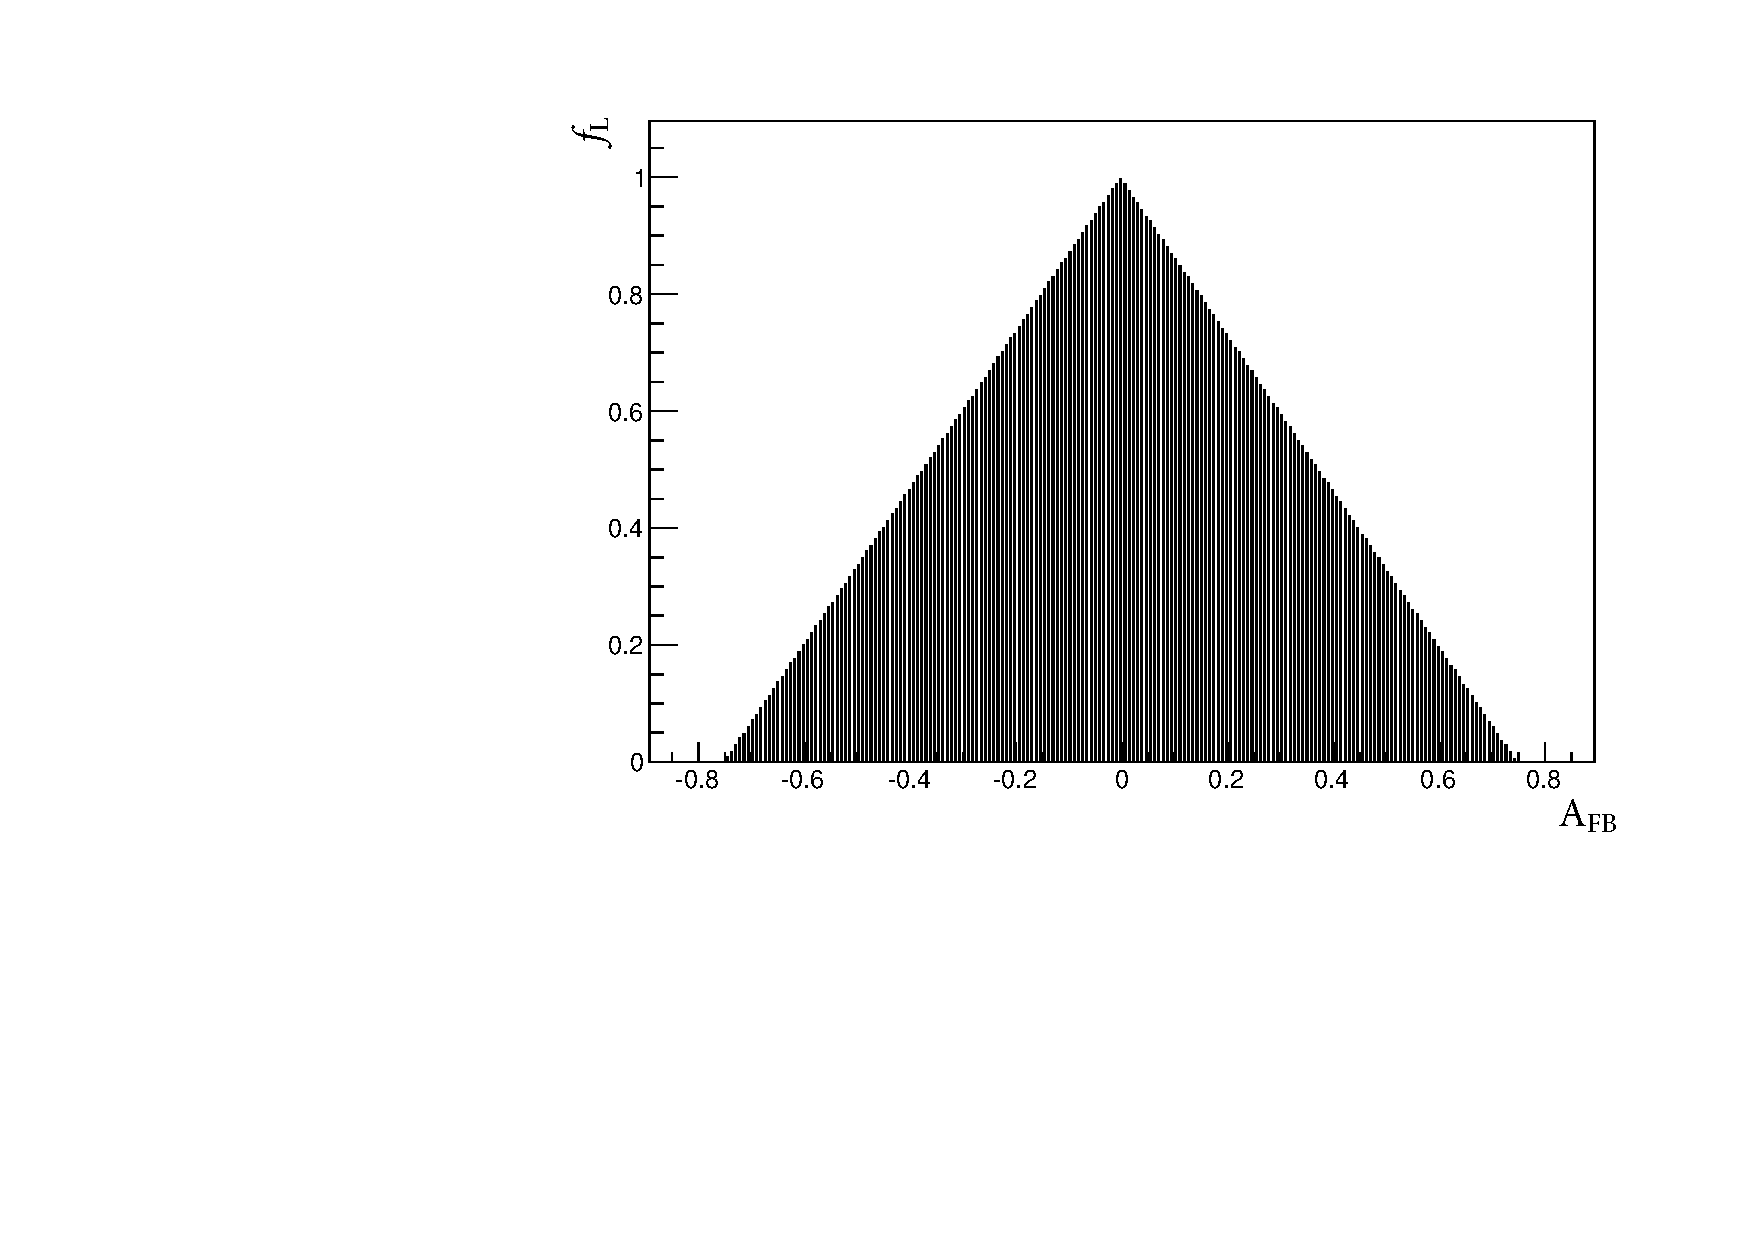
\includegraphics[width=0.8\textwidth]{Lmumu/figs/scan.pdf}
\caption{The plot shows the physical $A_{FB}^\ell$ vs $f_L$ parameter space. The dark region corresponds to points where the pdf is positive in the whole $[-1,1]$ interval. }
\label{fig:pdfscan}
\end{figure}
%
\begin{figure}[h!]
\centering
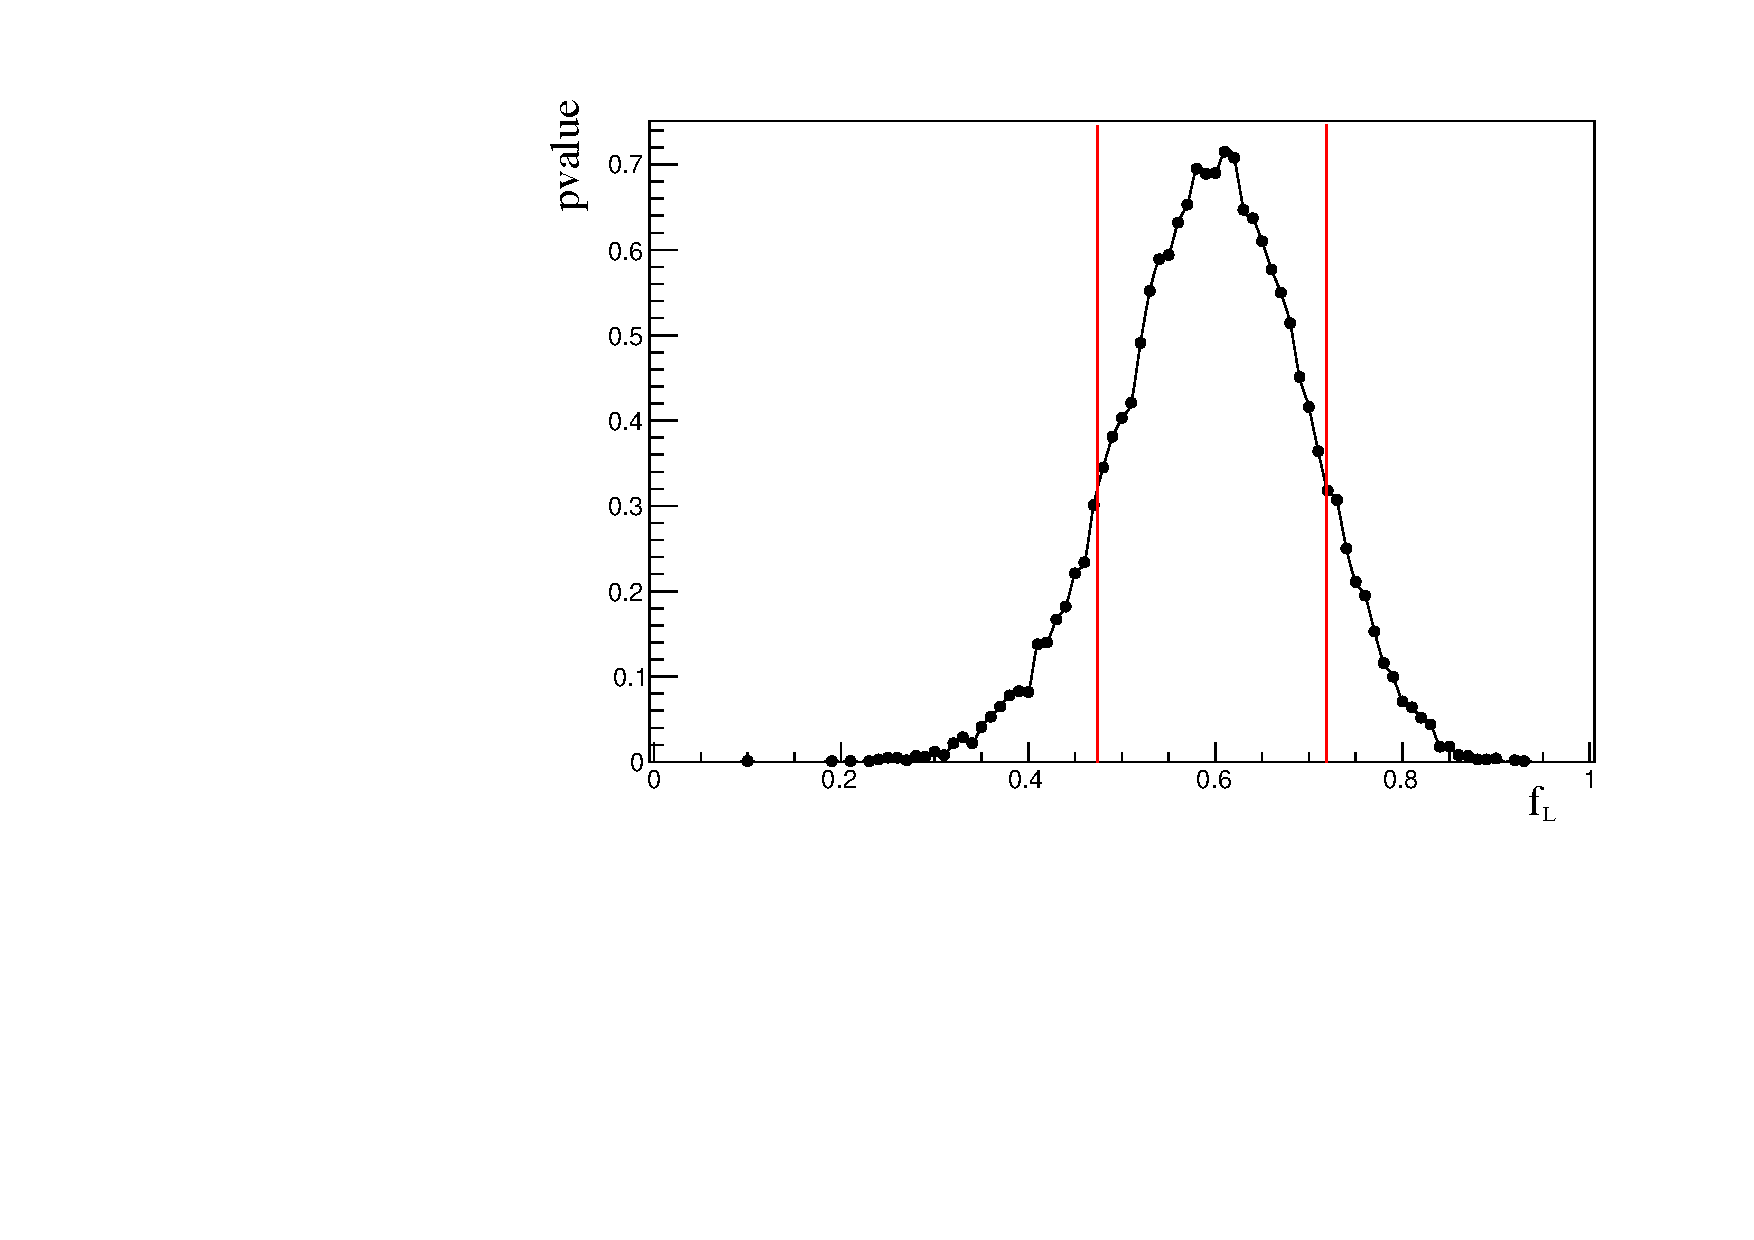
\includegraphics[width=0.45\textwidth]{Lmumu/figs/pvalue_fL_1500_2000.pdf}
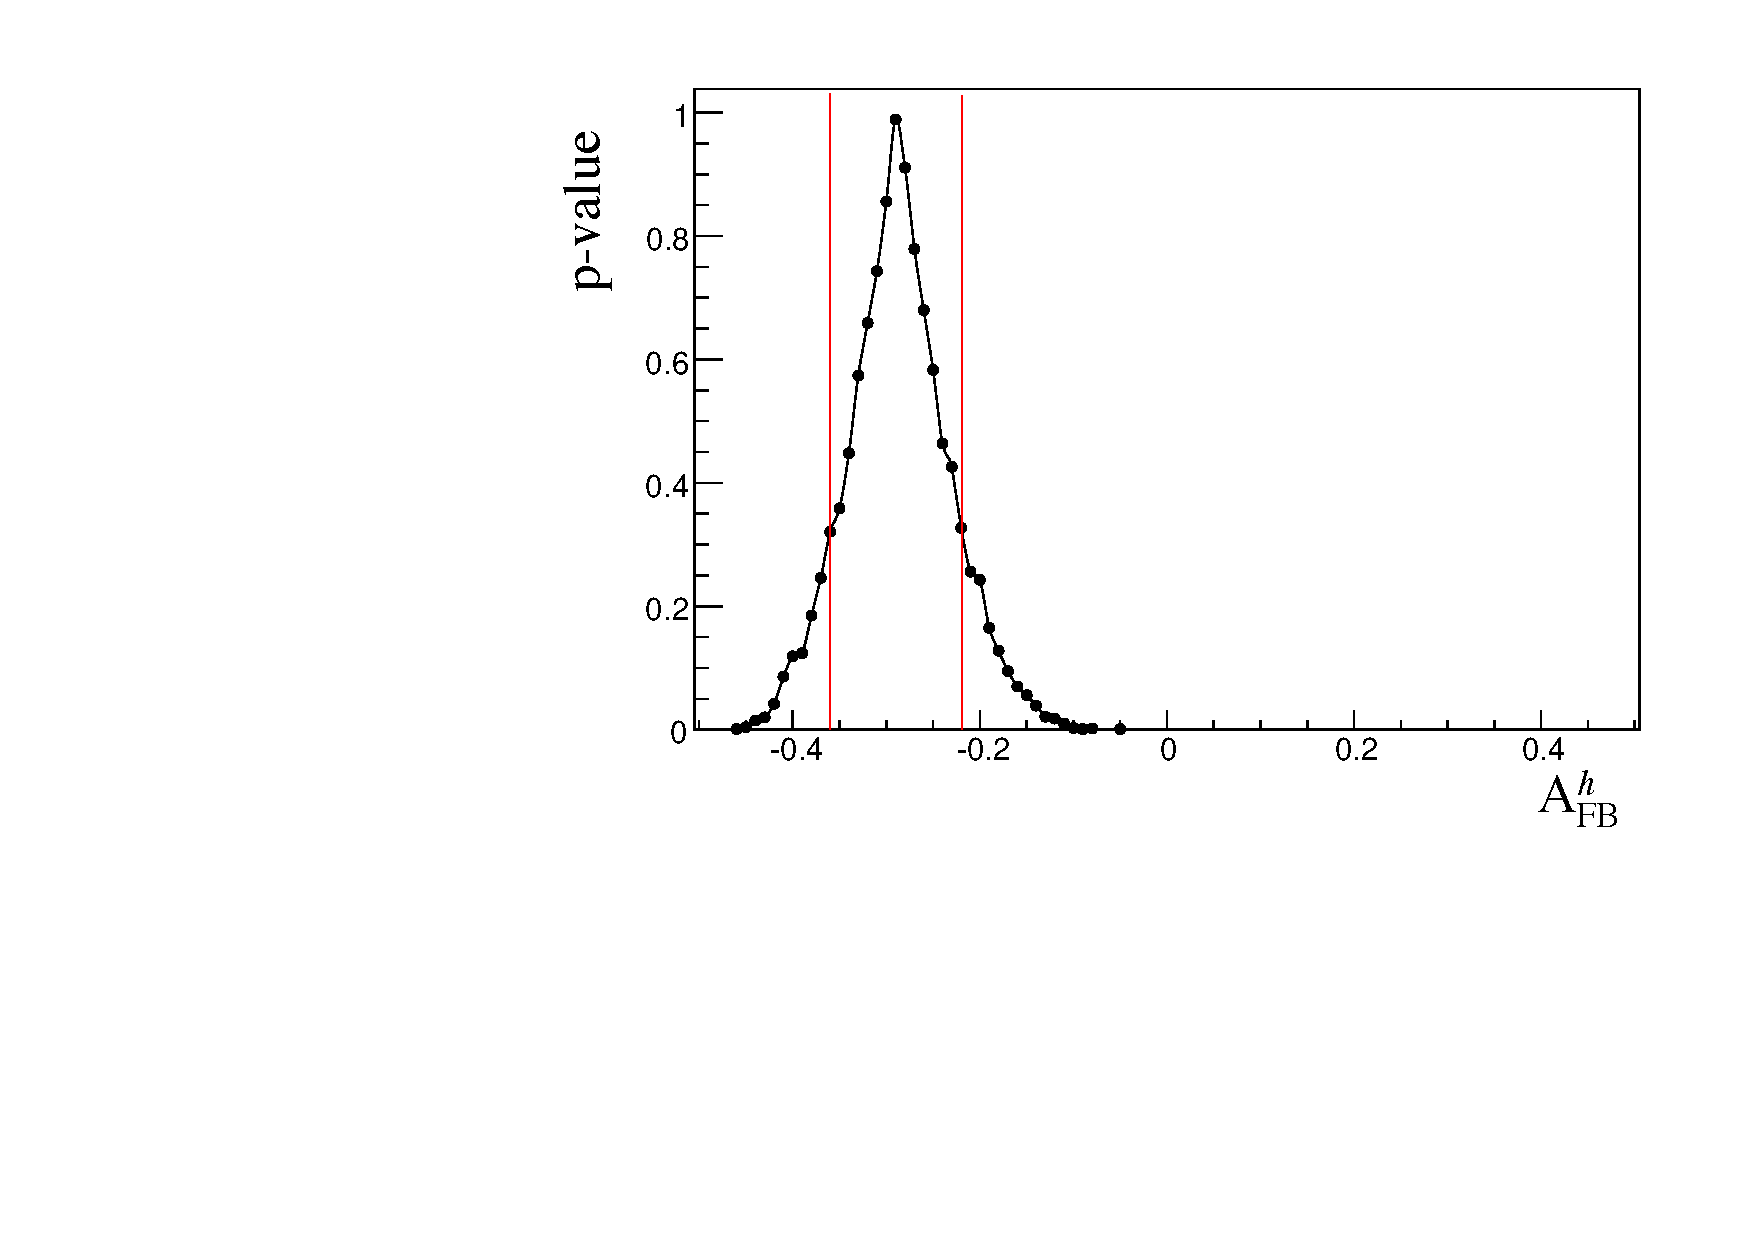
\includegraphics[width=0.45\textwidth]{Lmumu/figs/pvalue_afbB_1500_2000.pdf}
\caption{ p-values obtained with the plug-in method around the measured values in the 
high \qsq integrated bin for $f_{L}$ (left) and $A_{FB}^h$ (right).
The red line marks the points at p-value 32\% corresponding to a 68\% CL. }
\label{fig:FCexample}
\end{figure}

\section{Modelling the angular distributions}

The observables are extracted from fits to one-dimensional angular distributions.
%
%The function describing the $\cos\theta_\ell$ distribution, used to extract $A_{\rm FB}^\ell$ is 
%given by (for details, see appendix \ref{ap:angObservables})
%\begin{align}
%\frac{d\Gamma(\Lambda_{b}\to \Lambda \,\ell^{+}\ell^{-})}{dq^2d\cos\theta_\ell}=
%\frac{d\Gamma}{dq^2}&\left[  \frac{3}{8}\left(1+\cos^2\theta_\ell\right)(1-f_L)+A_{FB}^\ell\cos\theta_\ell +
%   \frac{3}{4}f_L \sin^2\theta_\ell \right], 
%\label{eq:afbLTh}
%\end{align}
%where $f_{\rm L}$ is fraction of longitudinally polarised dimuons.
%The distribution for the hadronic side has form
%\begin{equation}
%\frac{d\Gamma(\Lambda_{b}\to \Lambda(\to p \pi^{-})\ell^{+}\ell^{-})}
%     {dq^2\,d\cos\theta_\Lambda} 
%={\rm Br}(\Lambda \to p\pi^{-})
% \frac{d\Gamma(\Lambda_b \to \Lambda\, \ell^{+}\ell^{-})}{d q^2}\frac{1}{2}
%\Big(1+2A_{FB}^h\cos\theta_\Lambda\Big) \,. 
%\label{eq:afbBTh}
%\end{equation}
%
The PDFs used to model the data is defined as
%
\begin{equation}
P^k(\cos\theta_{\ell/h}) = f_b P_S(\cos\theta_{\ell/h}) \times \varepsilon^k(\cos_{\theta_{\ell/h}}) + 
		(1-f_b)P_B^k(\cos\theta_{\ell/h}),
\end{equation}
%
where $k=$(LL,DD), $P_S$ is the signal function composed by a theoretical shape given by Eq.~\ref{eq:afbBTh} and
\ref{eq:afbLTh} multiplied by an acceptance function $\varepsilon$ described in Sec.~\ref{sec:AngEff}
and $P_B$ is a background component. To limit systemaitc effects due to the background parameterisation, 
the fit is performed in a restricted mass region around the peak:
$5580 < m(\Lz\mumu) < 5660 $ \mevcc ~(``signal region"), which is dominated by the signal.
%In this way in most of the \qsq bins we have $\sim 20\%$ of background events.
The background fraction, $f_b$, is fixed in the fit, by looking at the mass distribution 
in a wider mass interval and fitting it to extract the fraction of background in the signal region.
The background shape is parameterised with a linear function times the efficiency shape.
A different efficiency shape is used for downstream and long events and for each q2 bin.
The free parameter of this model is fitted on sideband candidates which contain only background
and fixed for the fit to the signal region. In Figs. \ref{fig:cosThetaLbkg} and \ref{fig:cosThetaBbkg} 
are reported the background distributions in the sideband ($m(\Lz\mumu) > 5700$ \mevcc)
for the high and low \qsq integrated intervals with overlaid the background functions alone.
In summary the only fit parameter in the total fit function is the forward-backward asymmetry.

\begin{figure}[h]
\centering
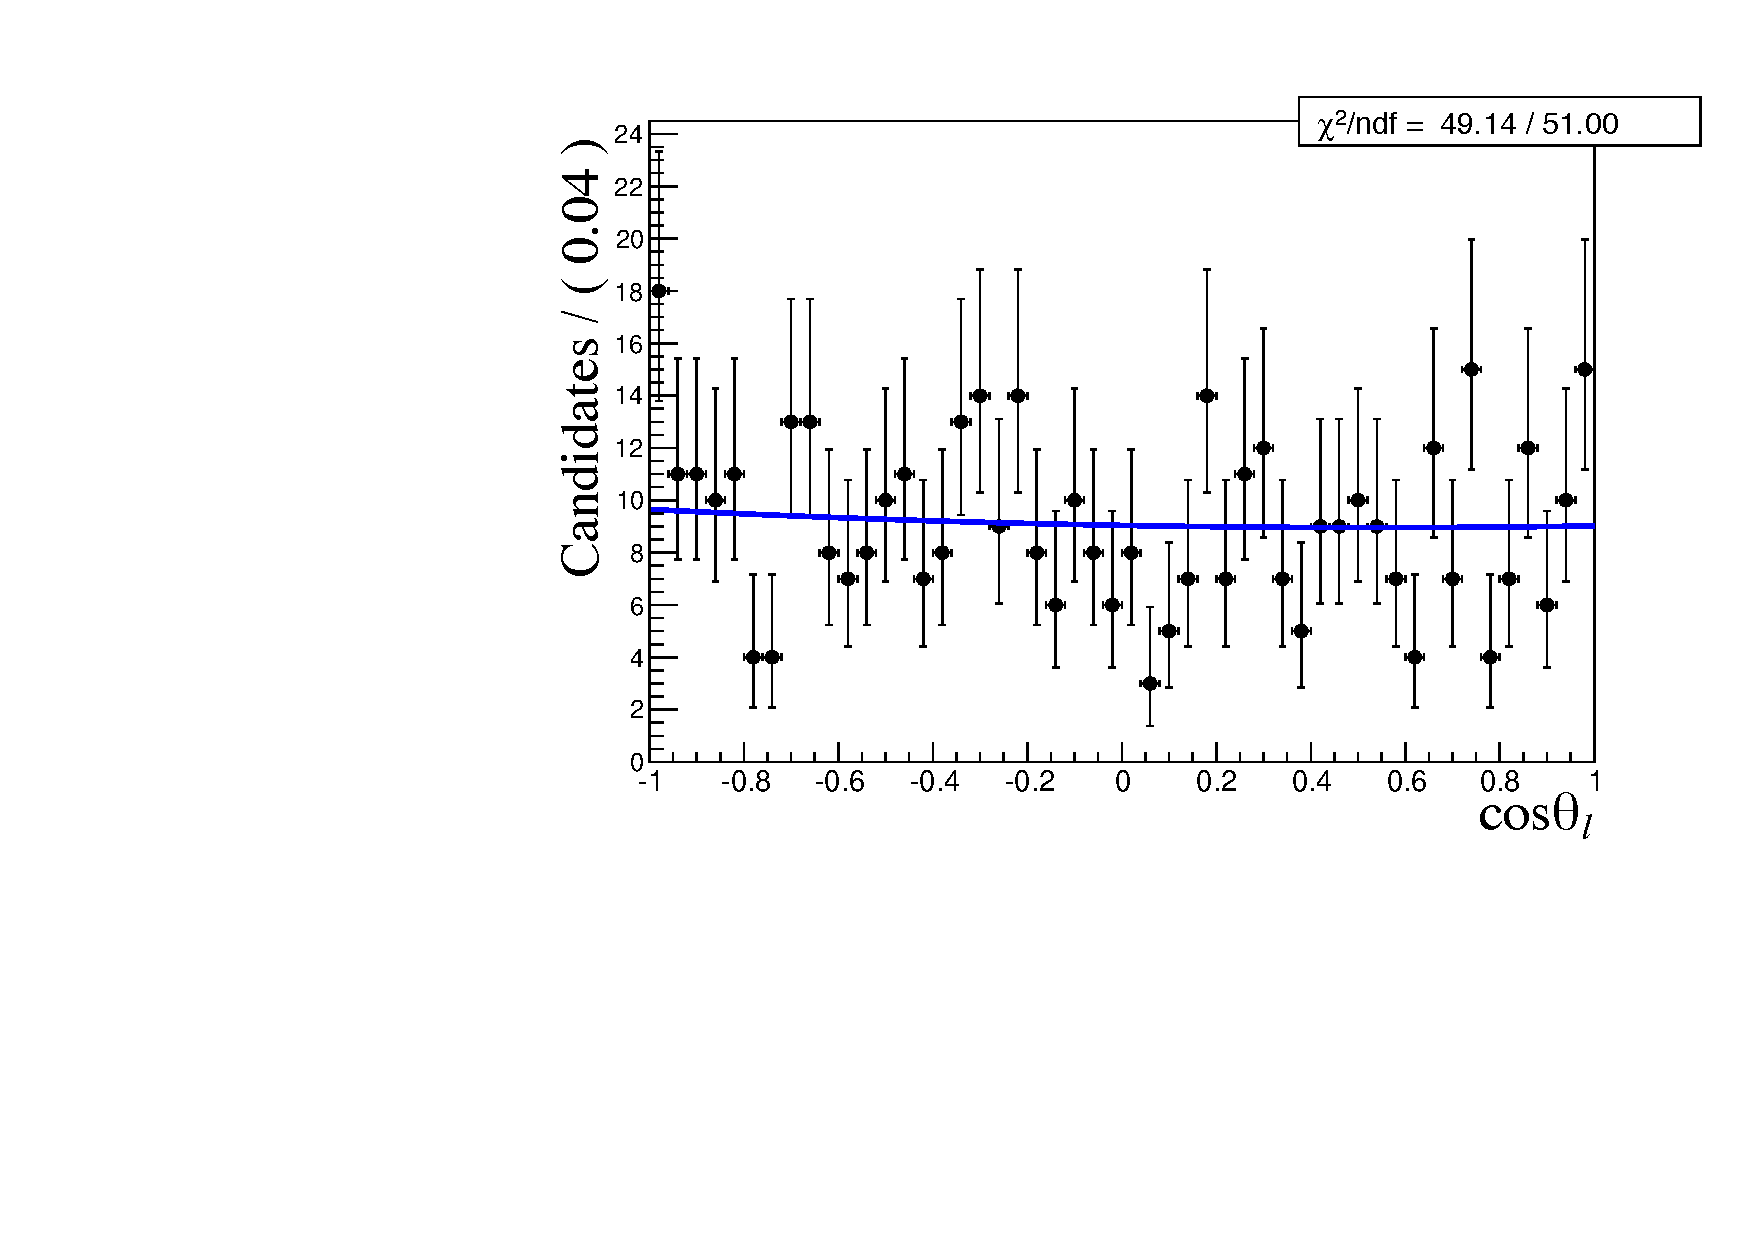
\includegraphics[width=0.45\textwidth]{Lmumu/figs/AngularBkgFits/BkgFit_highq2_DD.pdf}
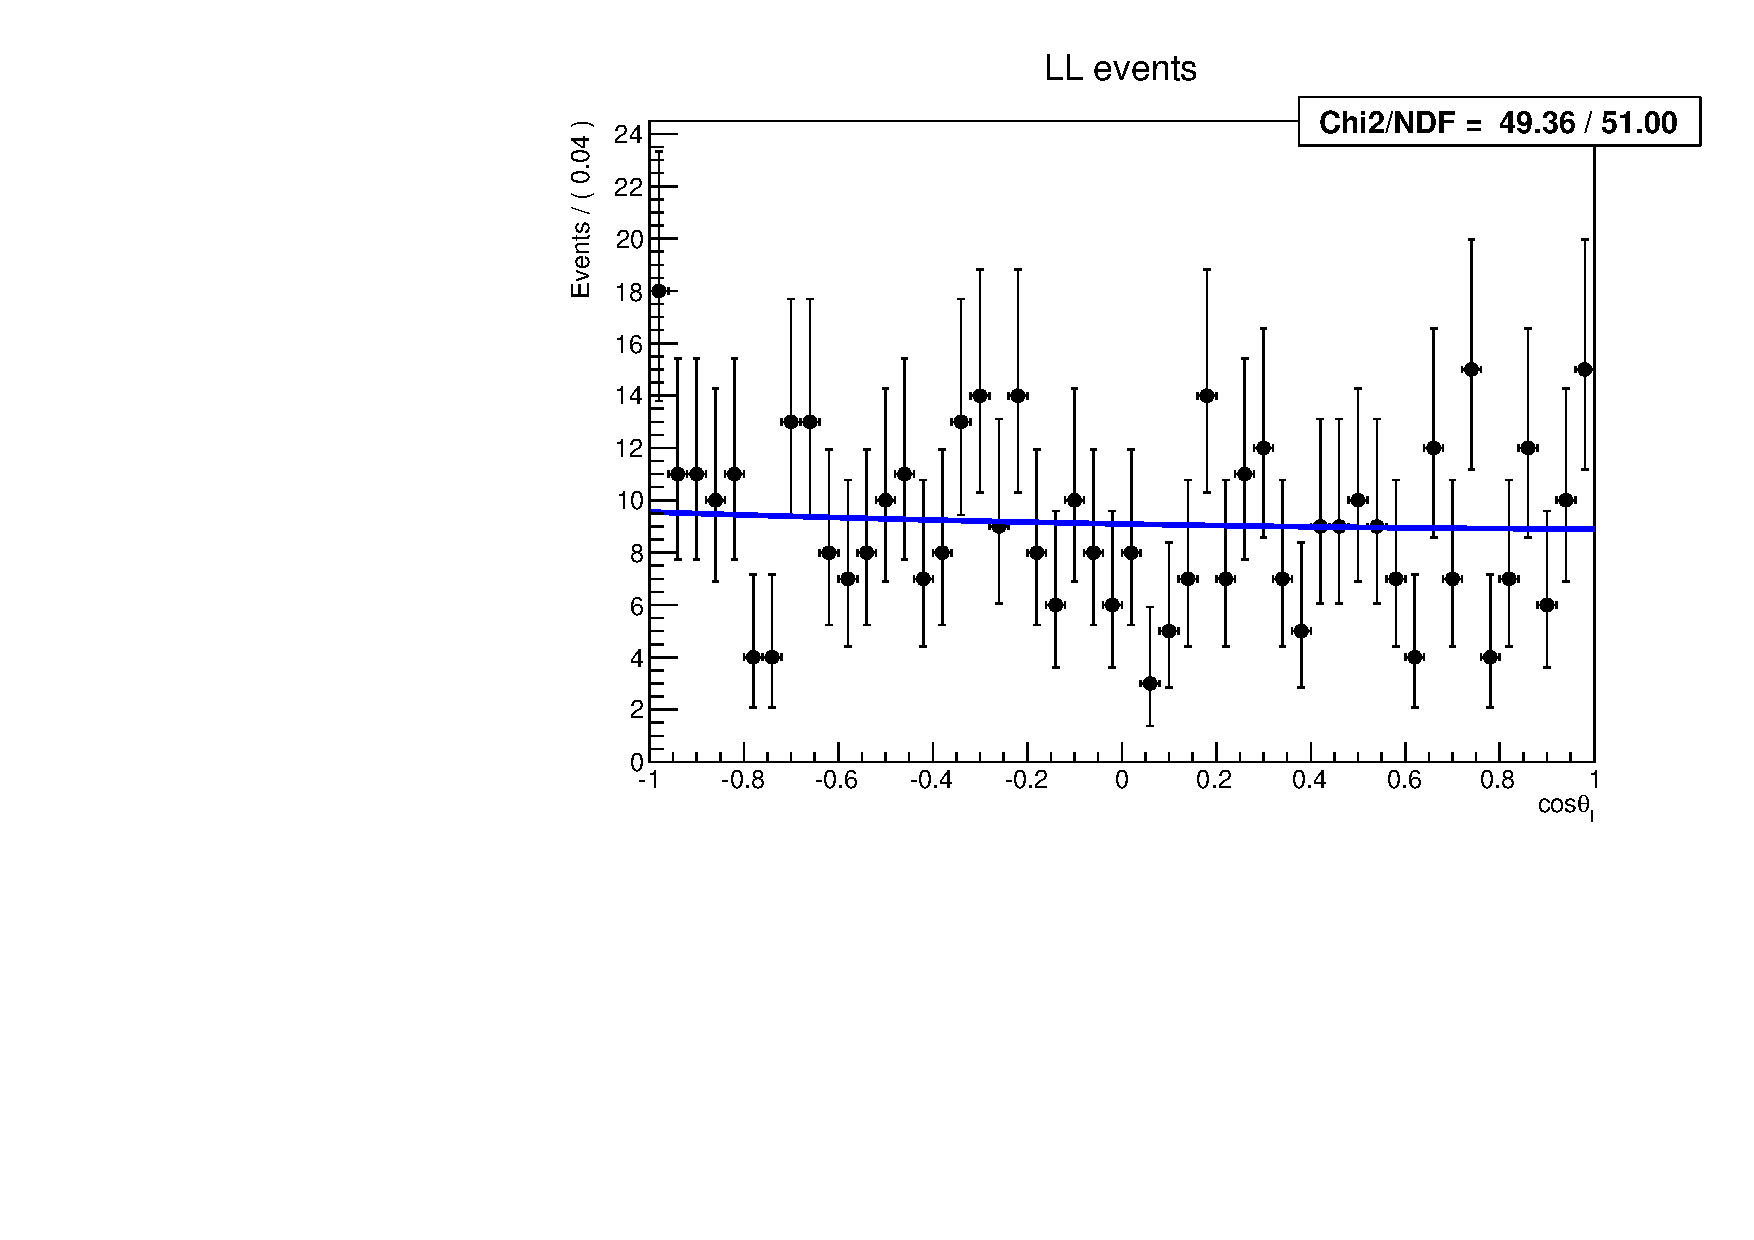
\includegraphics[width=0.45\textwidth]{Lmumu/figs/AngularBkgFits/BkgFit_highq2_LL.pdf}
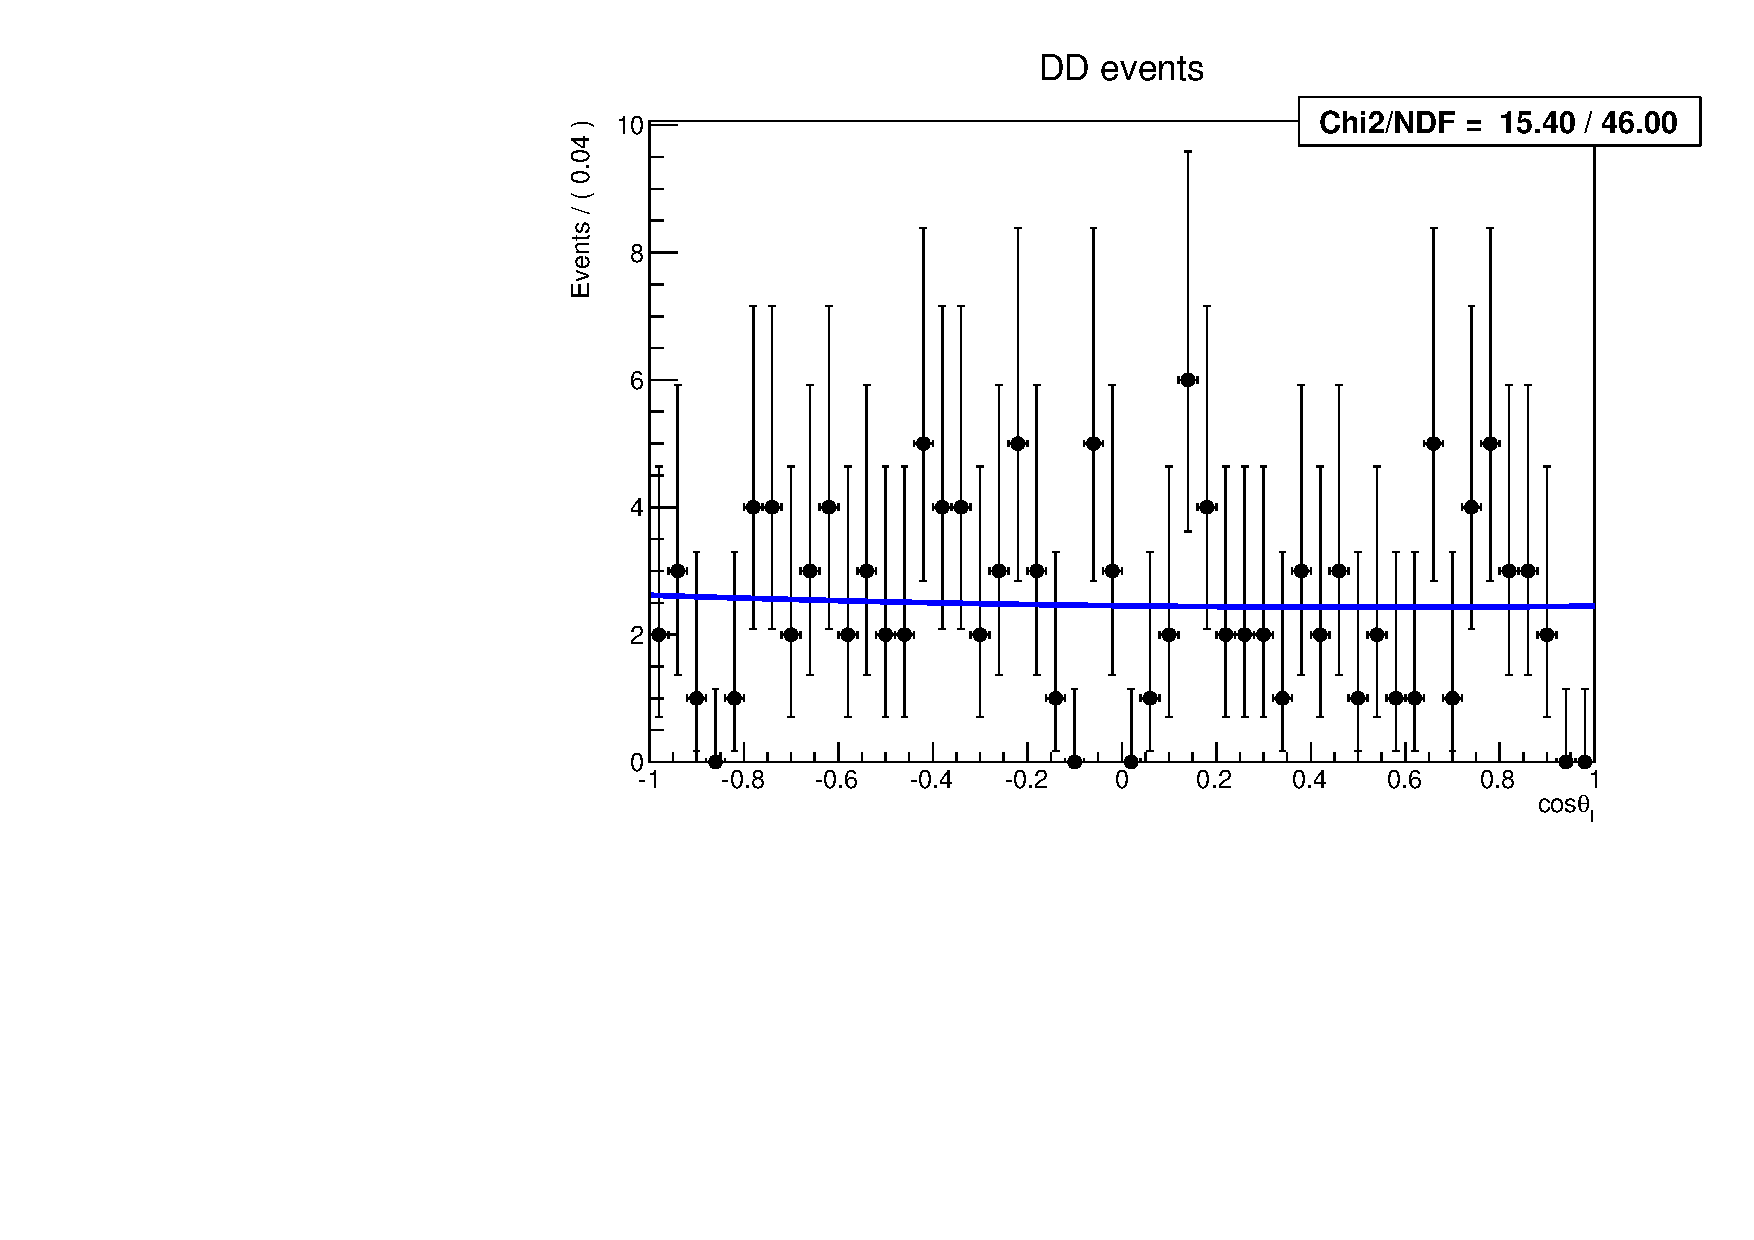
\includegraphics[width=0.45\textwidth]{Lmumu/figs/AngularBkgFits/BkgFit_lowq2_DD.pdf}
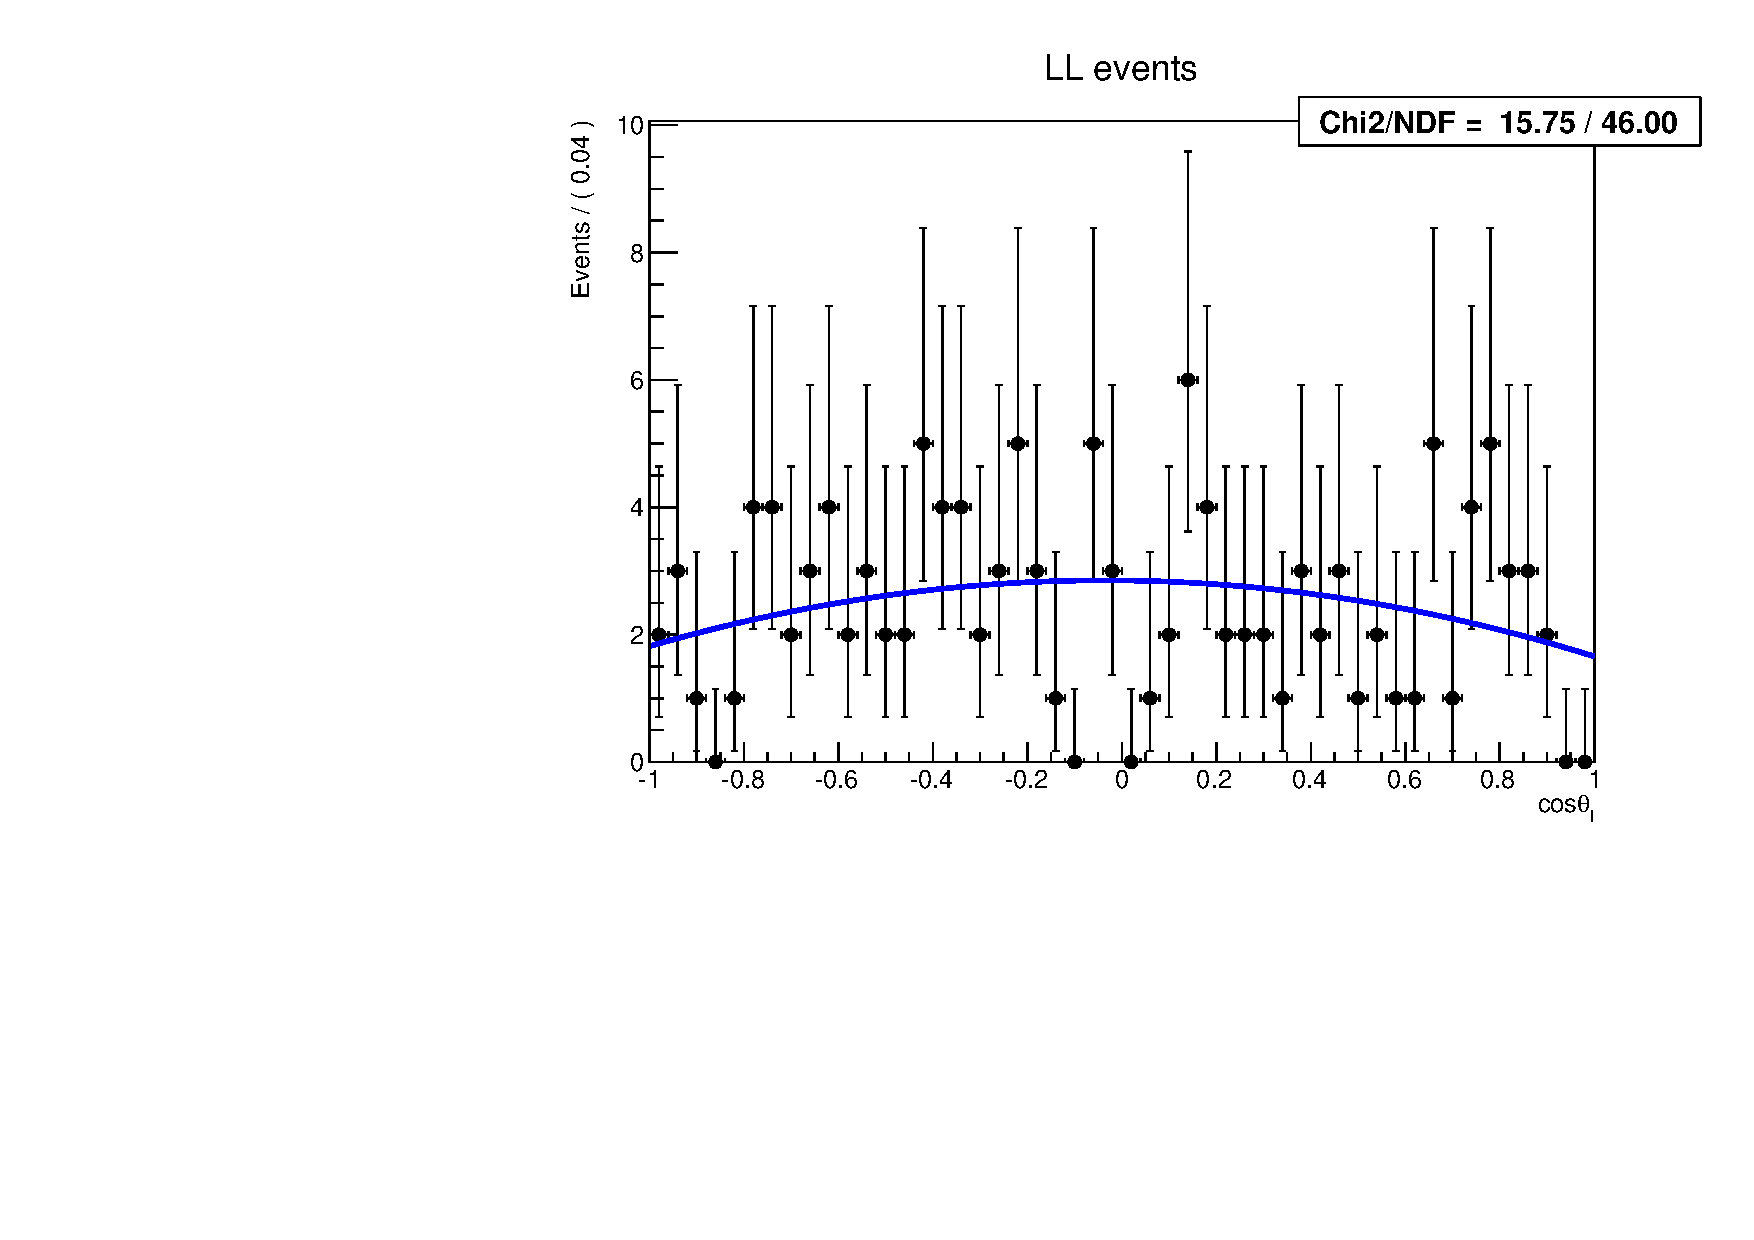
\includegraphics[width=0.45\textwidth]{Lmumu/figs/AngularBkgFits/BkgFit_lowq2_LL.pdf}
\caption{Background distribution as a function of $\cos\theta_\ell$ for downstream (left) and long (right)
events in the 15-20 \gevgevcccc (top) and 1.1-6 \gevgevcccc (bottom) \qsq bins.  }
\label{fig:cosThetaLbkg}
\end{figure}

\begin{figure}[h]
\centering
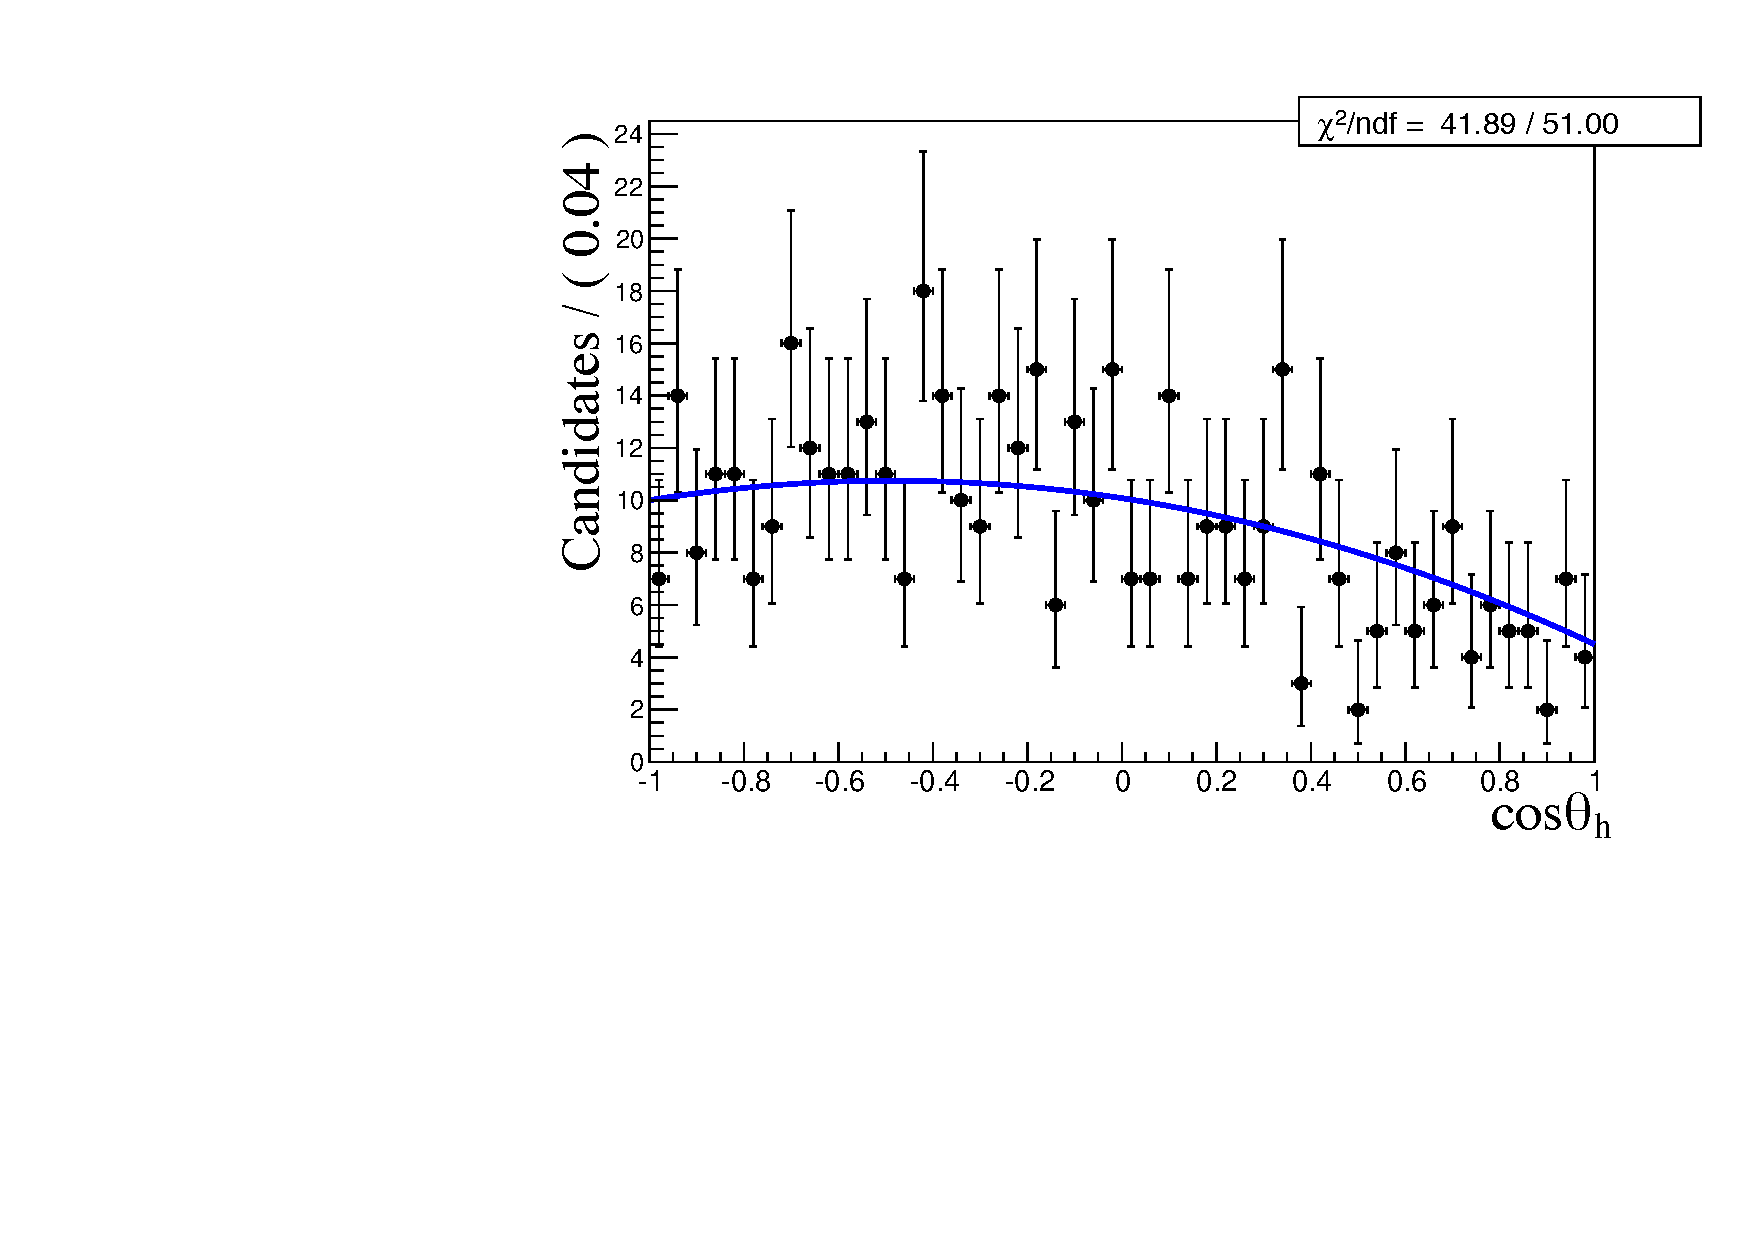
\includegraphics[width=0.45\textwidth]{Lmumu/figs/AngularBkgFits/BkgFitB_highq2_DD.pdf}
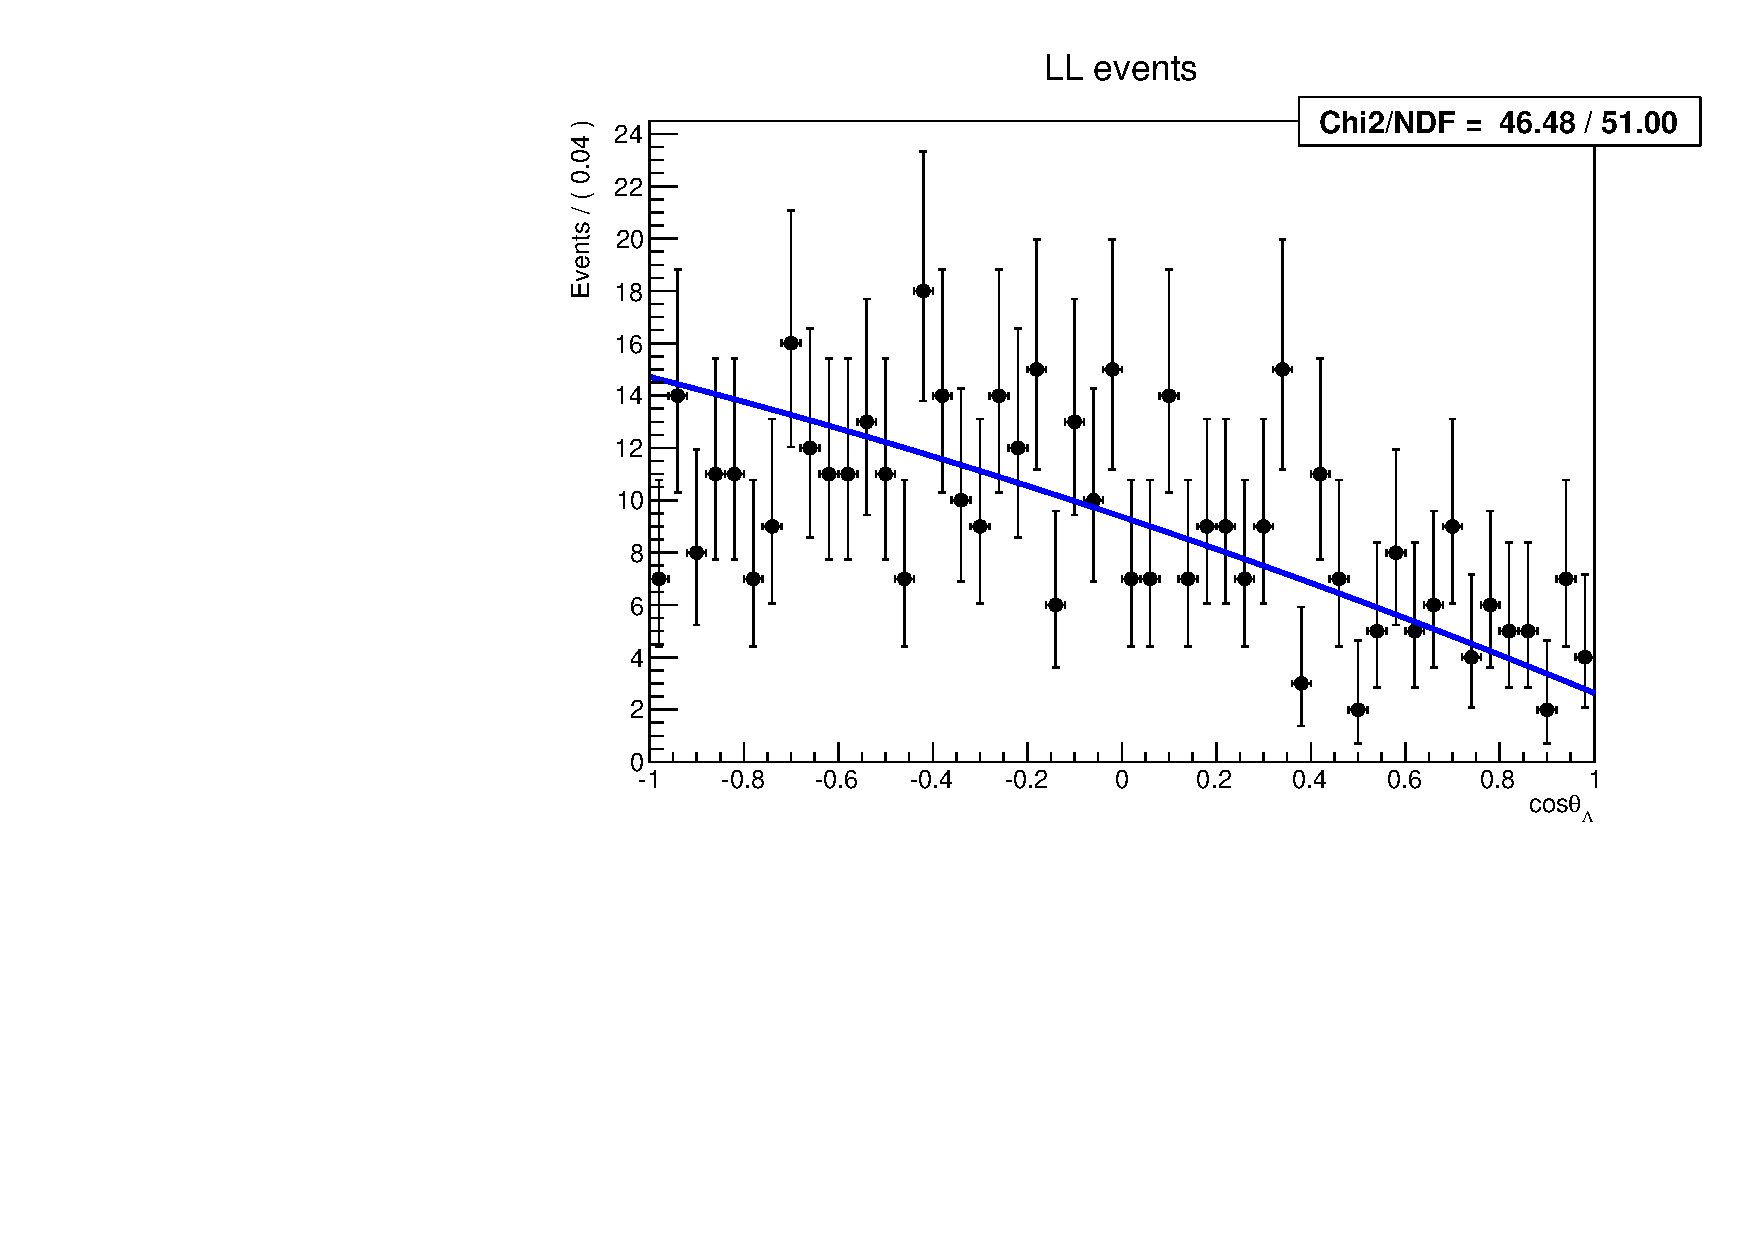
\includegraphics[width=0.45\textwidth]{Lmumu/figs/AngularBkgFits/BkgFitB_highq2_LL.pdf}
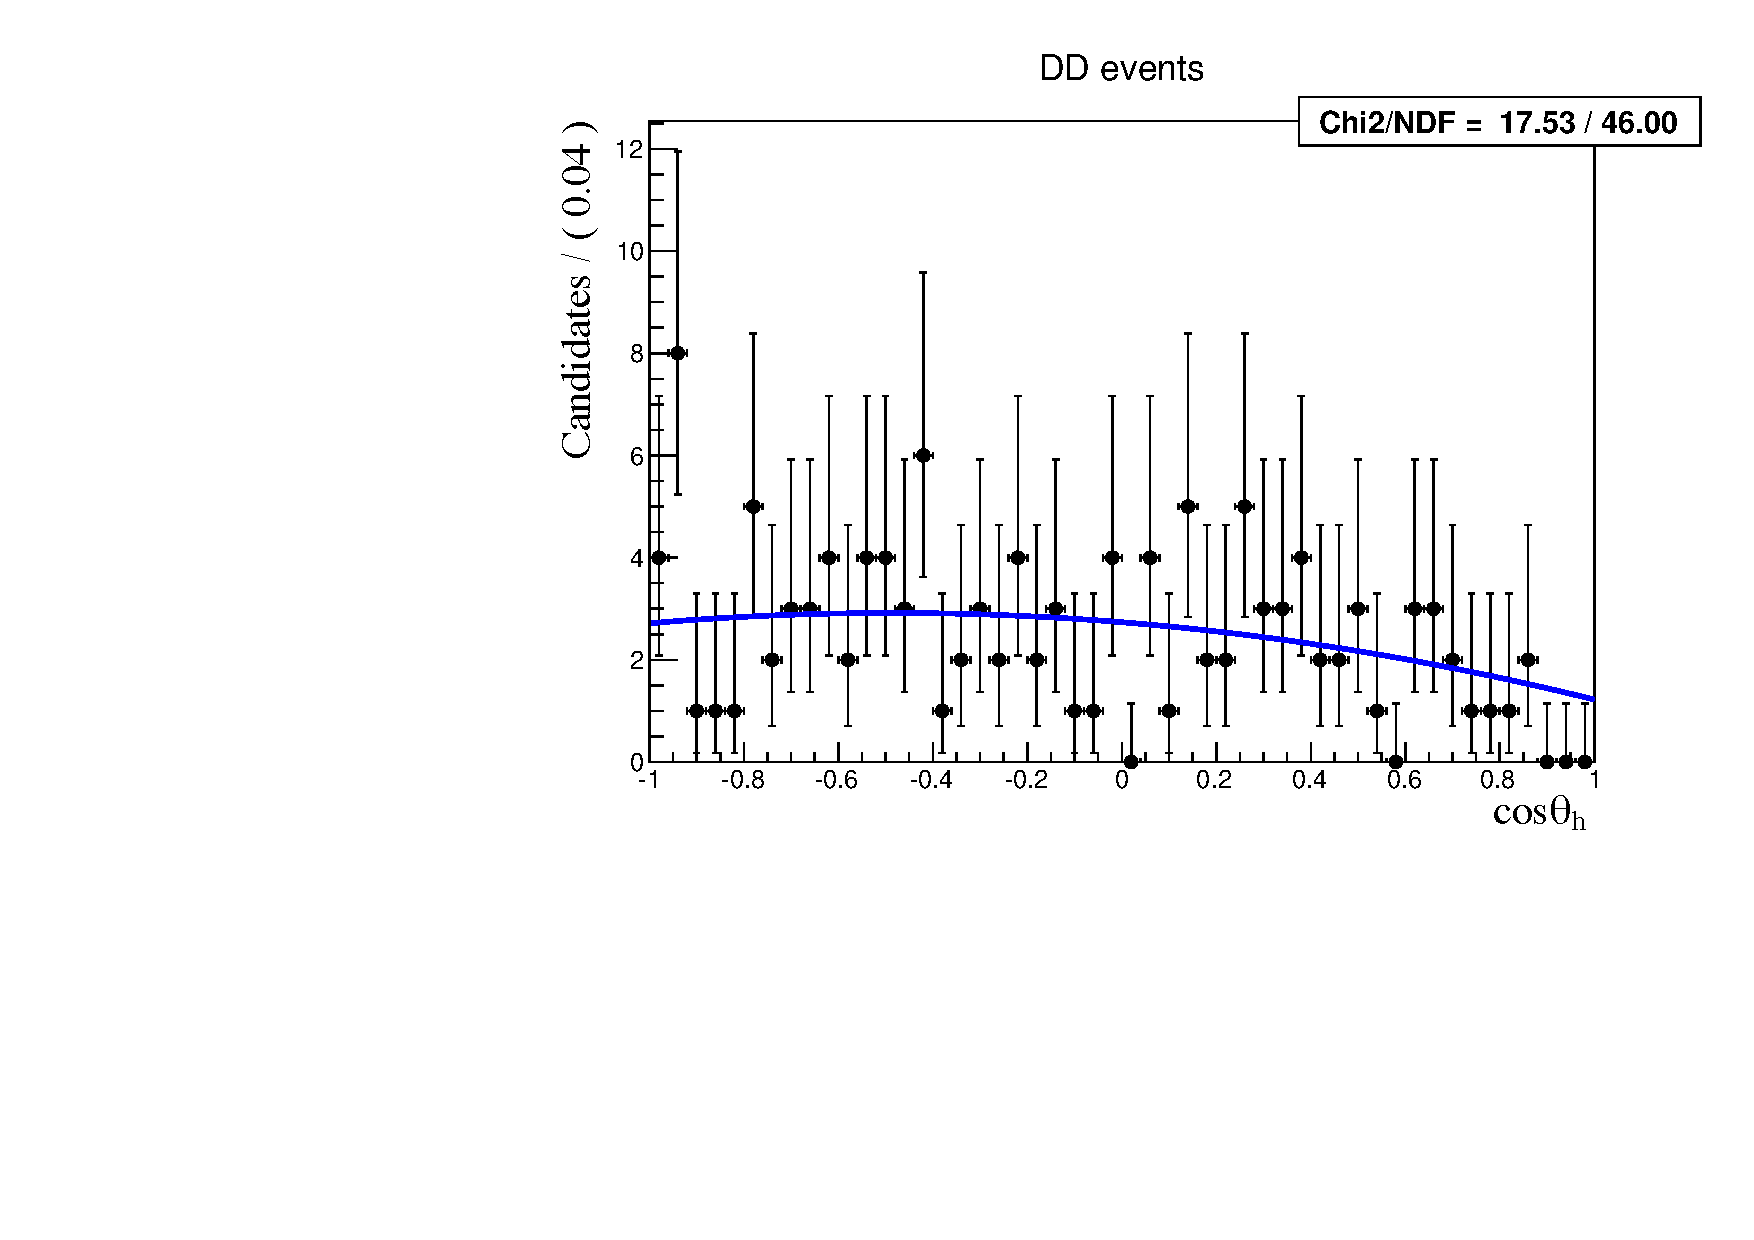
\includegraphics[width=0.45\textwidth]{Lmumu/figs/AngularBkgFits/BkgFitB_lowq2_DD.pdf}
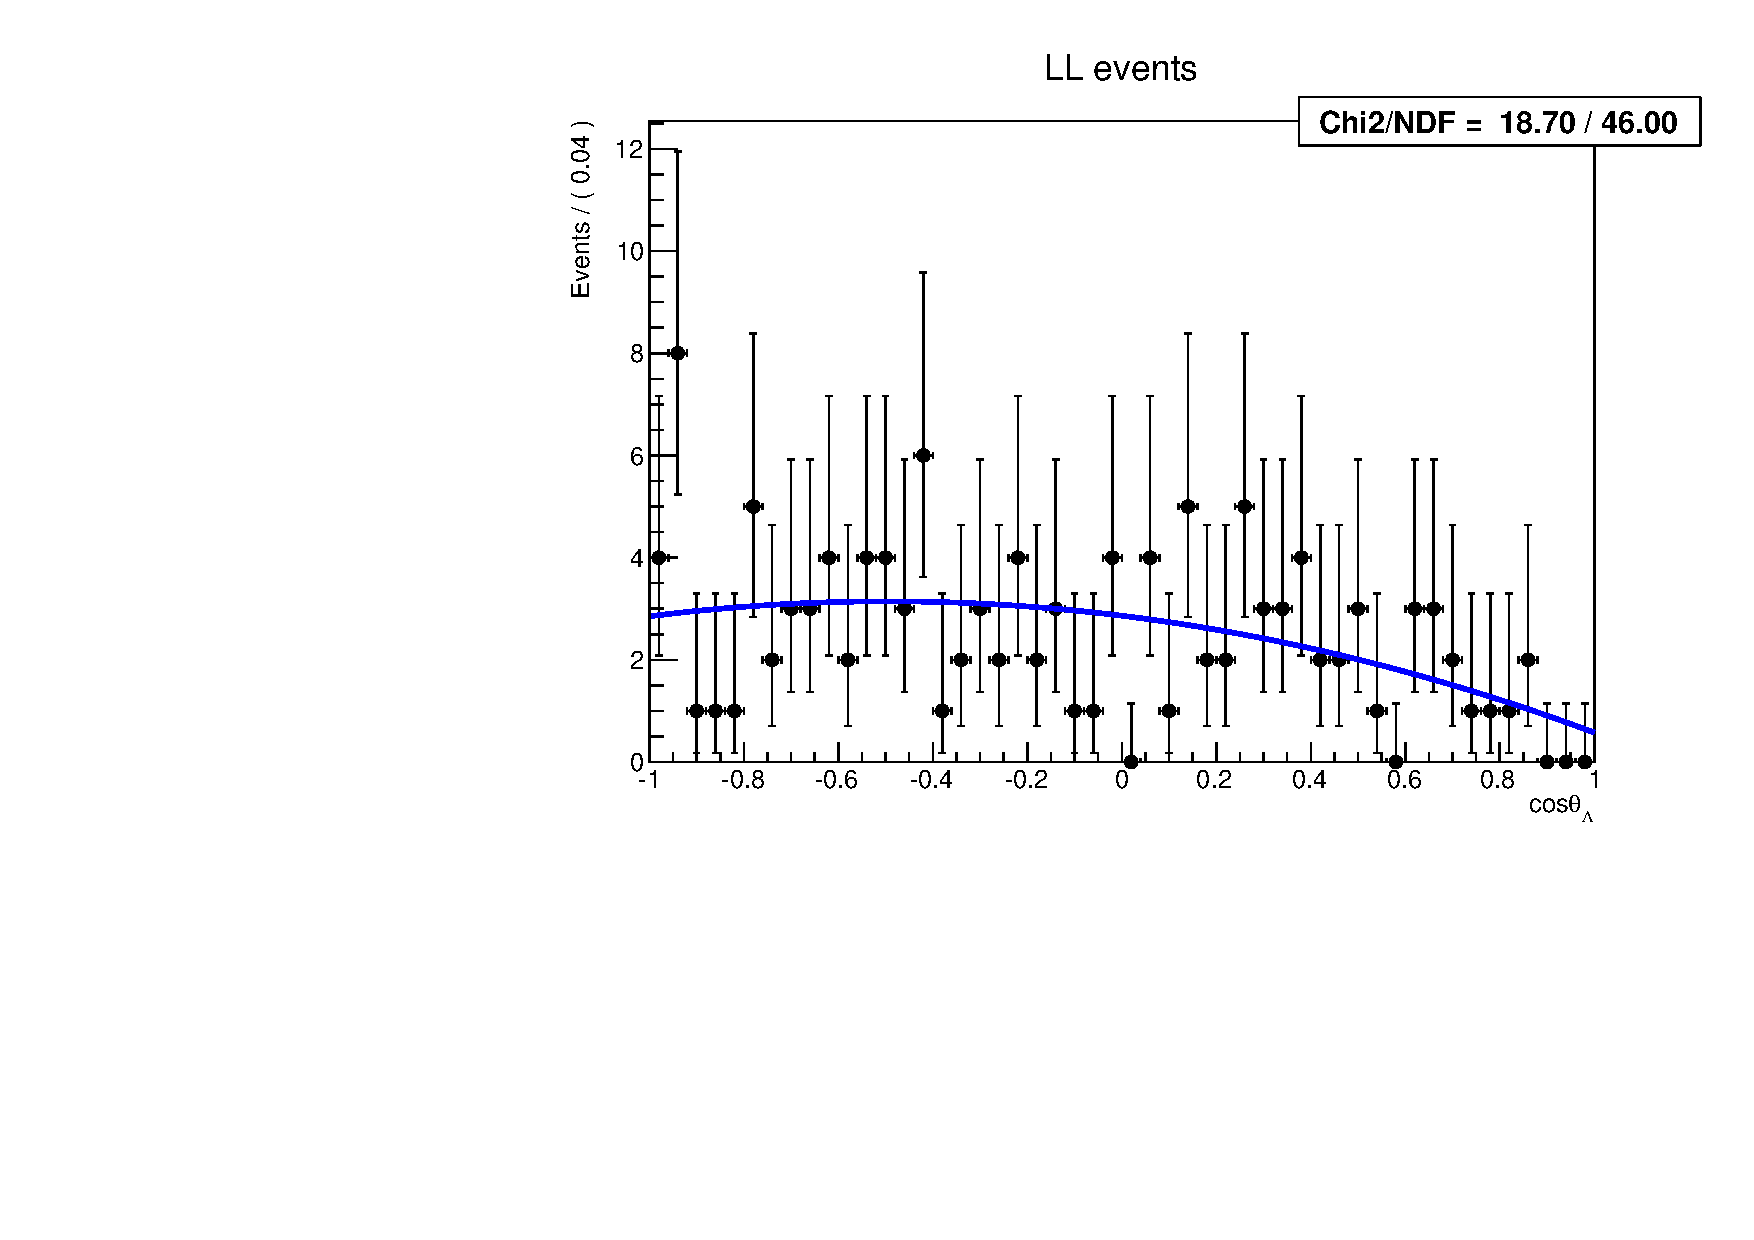
\includegraphics[width=0.45\textwidth]{Lmumu/figs/AngularBkgFits/BkgFitB_lowq2_LL.pdf}
\caption{Background distribution as a function of $\cos\theta_\Lambda$ for downstream (left) and long (right)
events in the 15-20 \gevgevcccc (top) and 1.1-6 \gevgevcccc (bottom) \qsq bins. }
\label{fig:cosThetaBbkg}
\end{figure}


\section{Angular acceptance}
\label{sec:AngEff}

Selection requirements on the minimum momentum of the muons may distort the $\cos \theta_\ell$ 
distribution by removing candidates with extreme values of $\cos\theta_\ell$. Similarly, 
the impact parameter requirements affect $\cos \theta_h$ as very forward hadrons tend
to have smaller impact parameter values. While in principle one could take it into account
by an additional weight, to minimise the distortion of the uncertainties estimate,
the efficiency function is incorporated in the fit model. The angular efficiency is
parametrised using a second-order polynomial and determined separately for downstream and
long candidates by fitting simulated events, with an independent set of parameters obtained
for each \qsq interval. These parameters are fixed in the fits to data.
Using polynomial functions allows to calculate the PDF normalisation analytically.
In Figs.~\ref{fig:cosThetaLeff} and \ref{fig:cosThetaBeffLow} efficiencies are reported,
as a function of $\cos\theta_h$ and $\cos\theta_\ell$ using \Lb\to\Lz\mumu simulated events
in the 15.0--20.0 and 1.1--6.0 \gevgevcccc integrated \qsq intervals.
%$\ref{fig:cosThetaLeffJpsi} and \ref{fig:cosThetaBeffJpsi} $J/\psi\Lz$ MC and $\Lz\mumu$ 
%
For the lepton side, even though the efficiency is symmetric by construction,
all parameters floating in the fit, namely it is not constrained to be symmetric.

\begin{figure}[h]
\centering
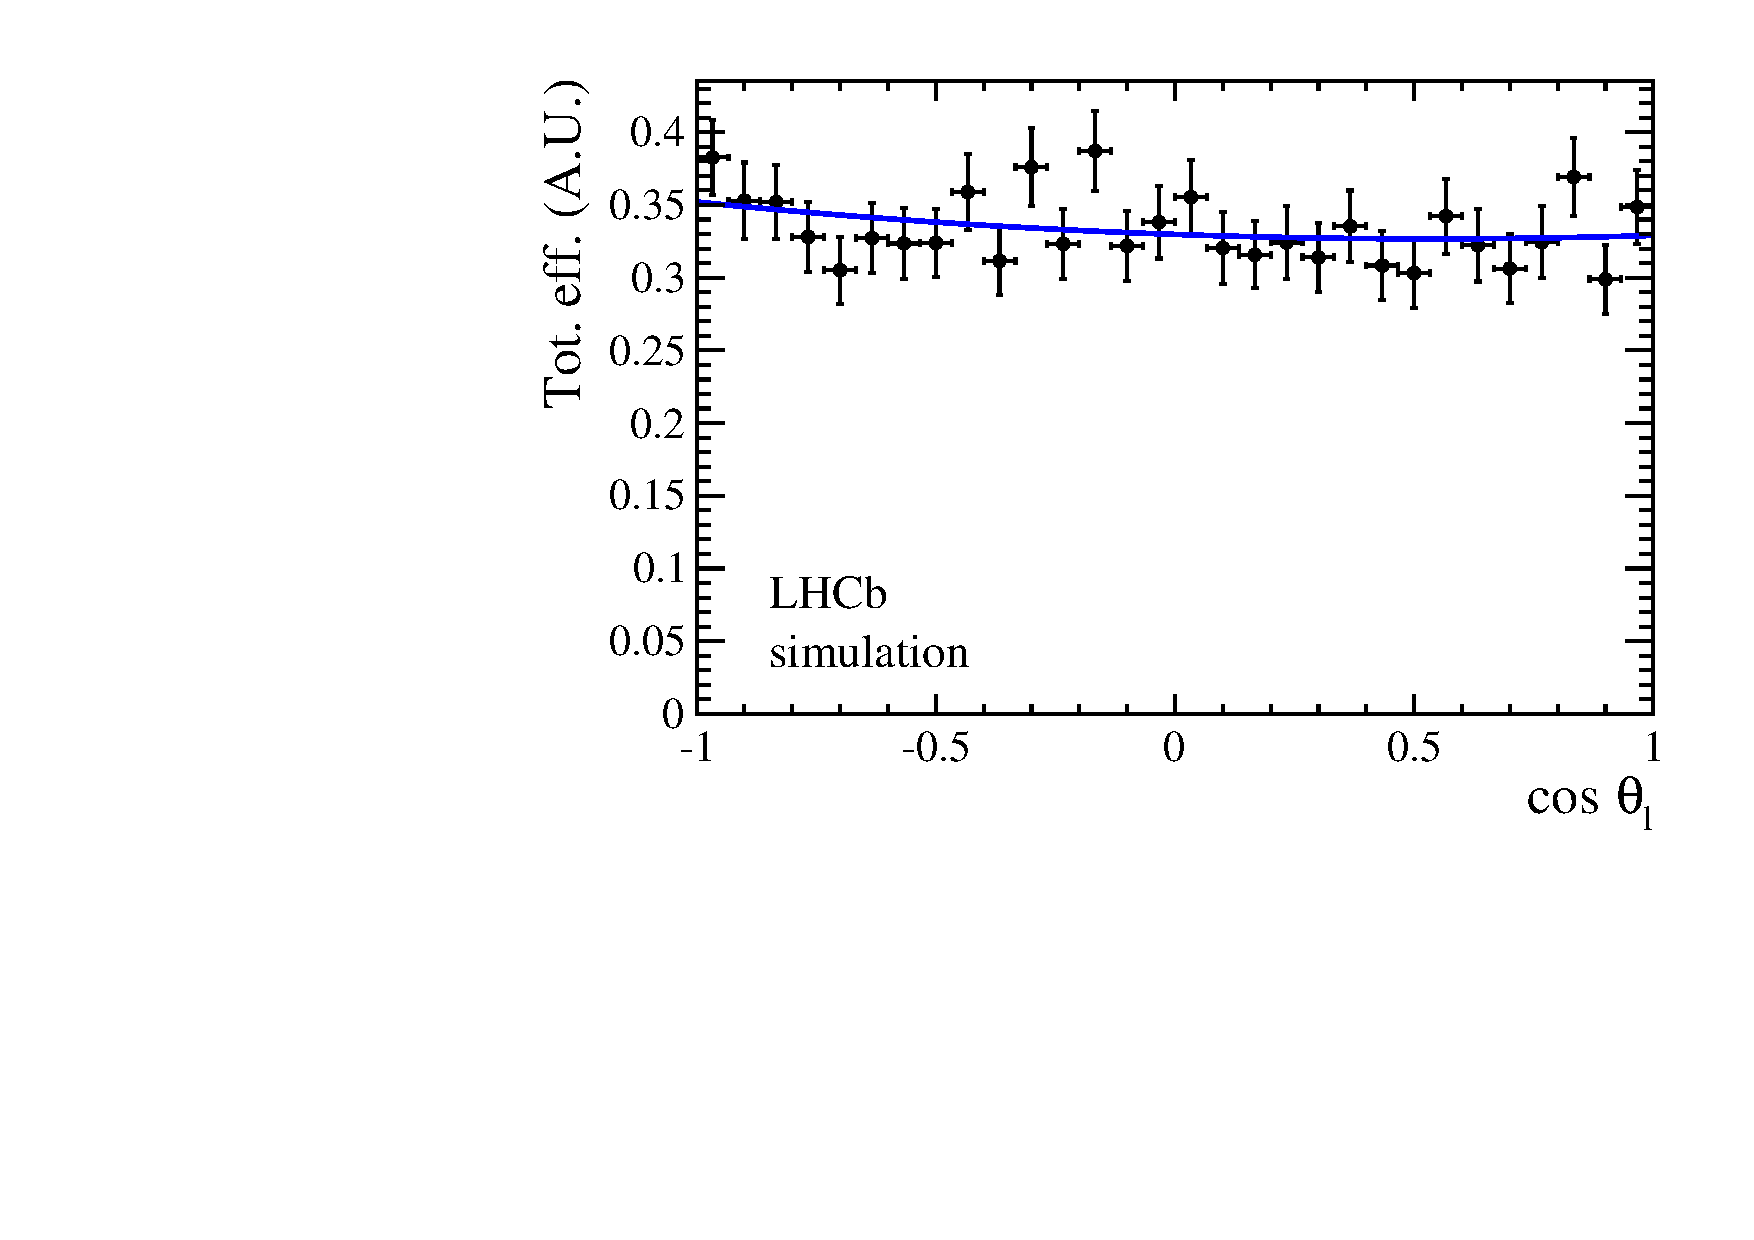
\includegraphics[width=0.45\textwidth]{Lmumu/figs/efficiencies/angular/DDeffFit_q2_1500_2000.pdf}
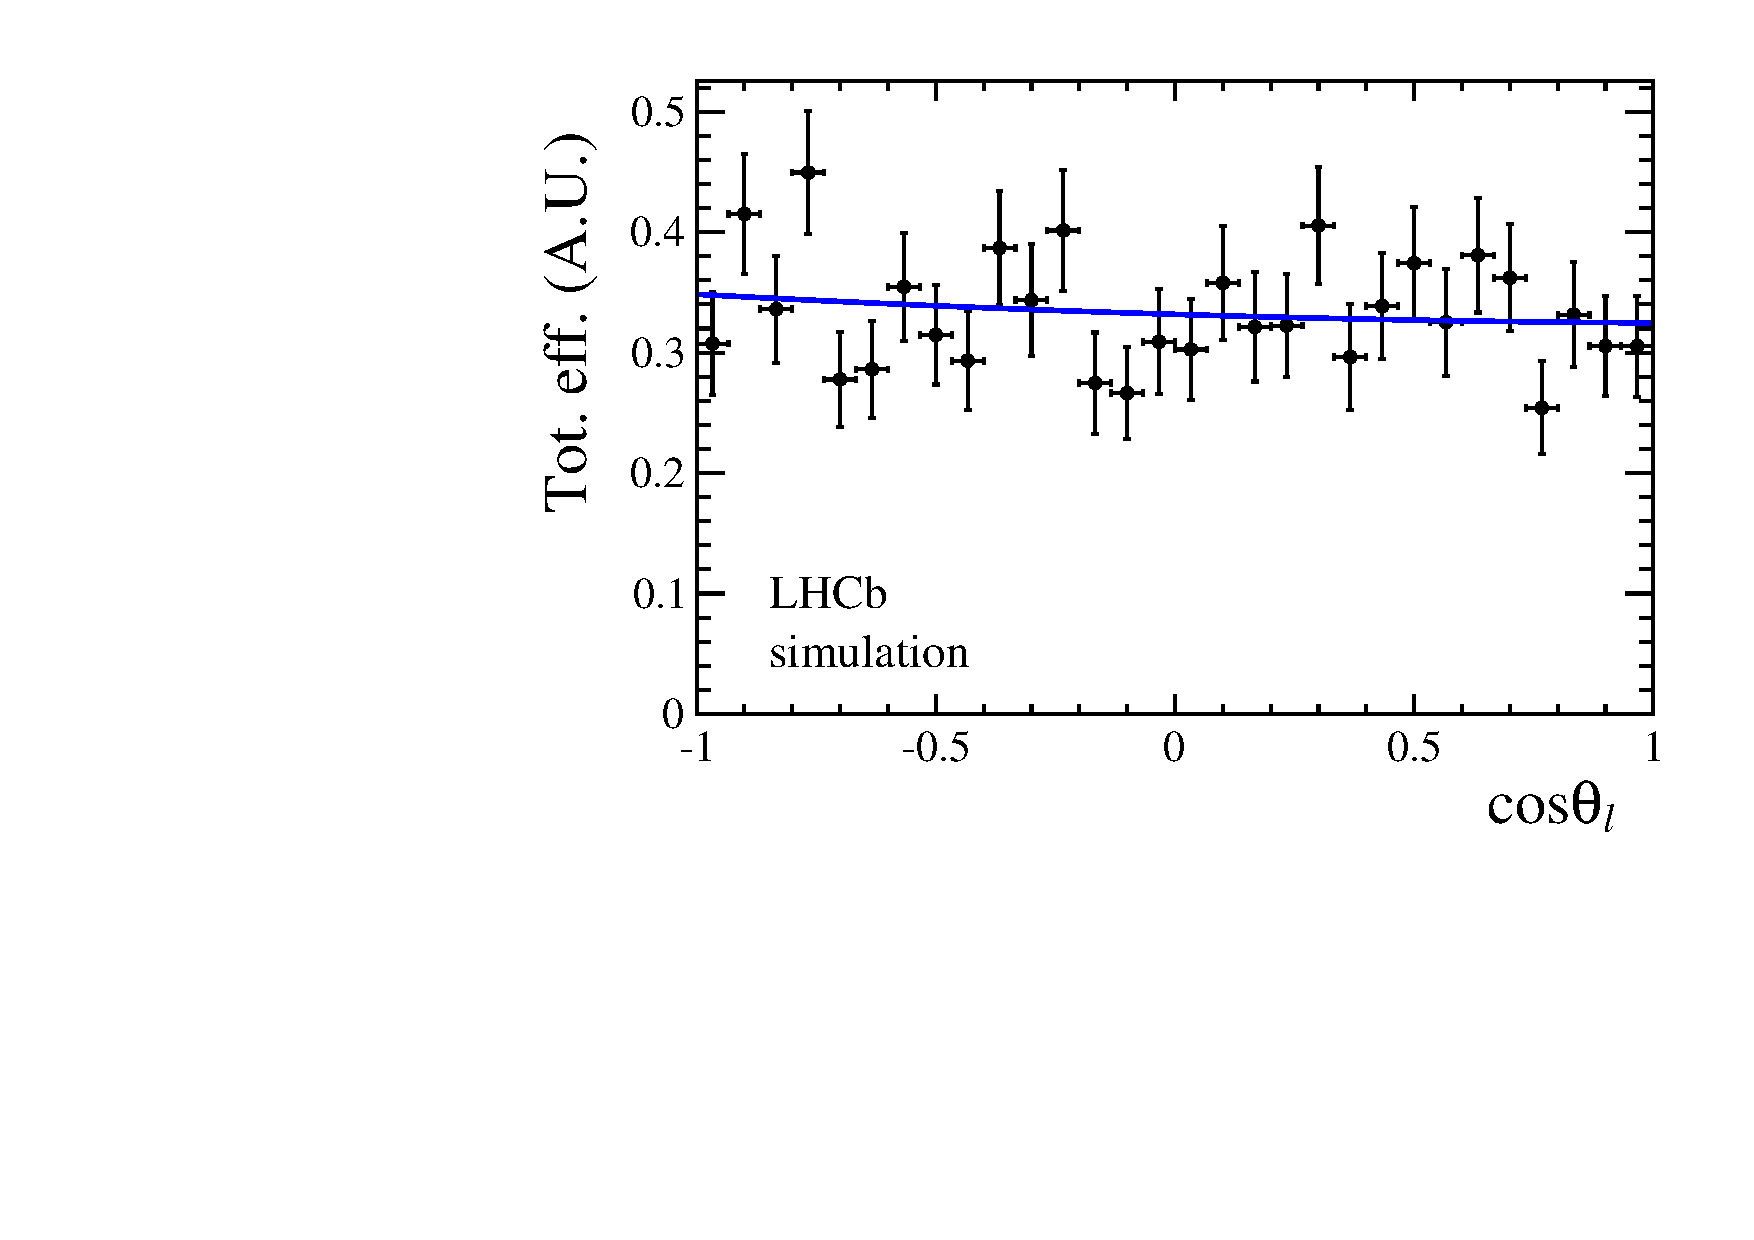
\includegraphics[width=0.45\textwidth]{Lmumu/figs/efficiencies/angular/LLeffFit_q2_1500_2000.pdf}
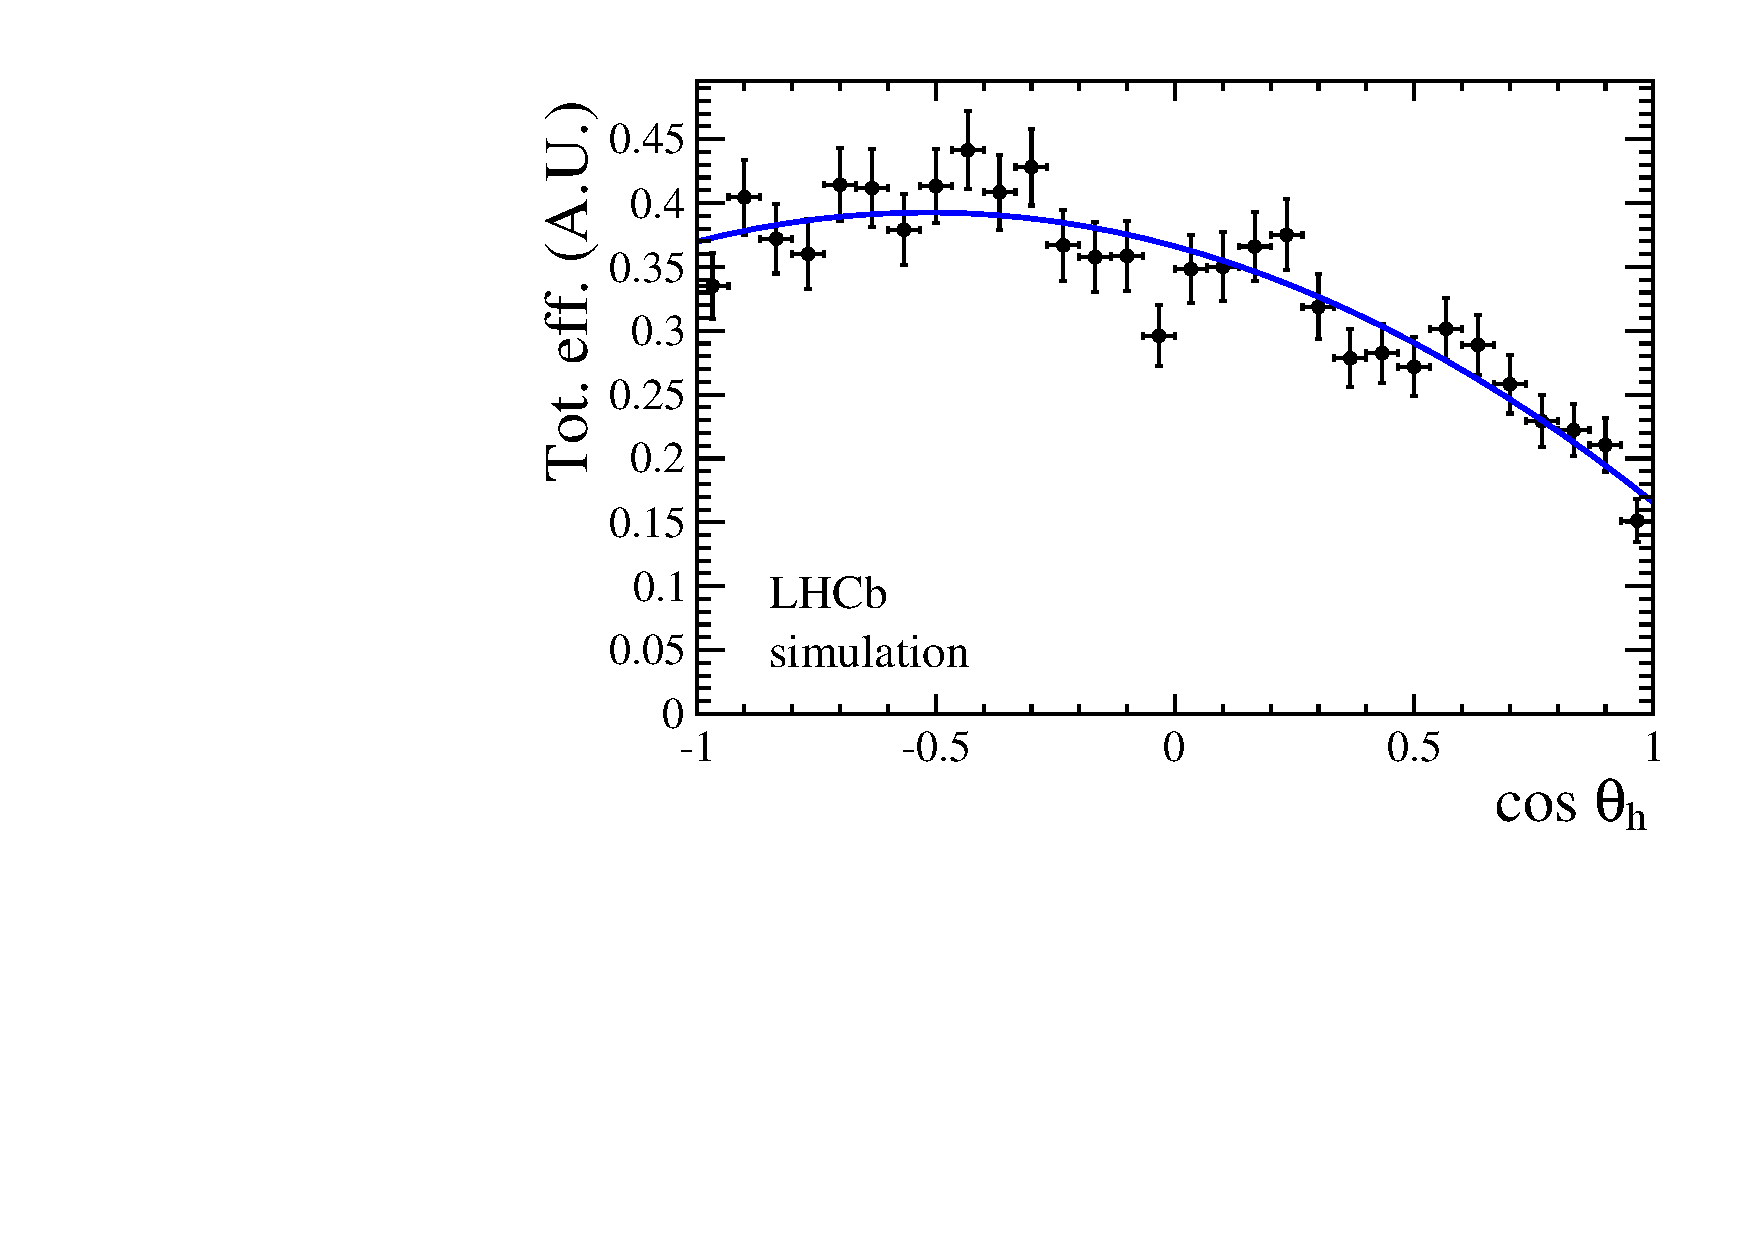
\includegraphics[width=0.45\textwidth]{Lmumu/figs/efficiencies/angular/DDeffFitB_q2_1500_2000.pdf}
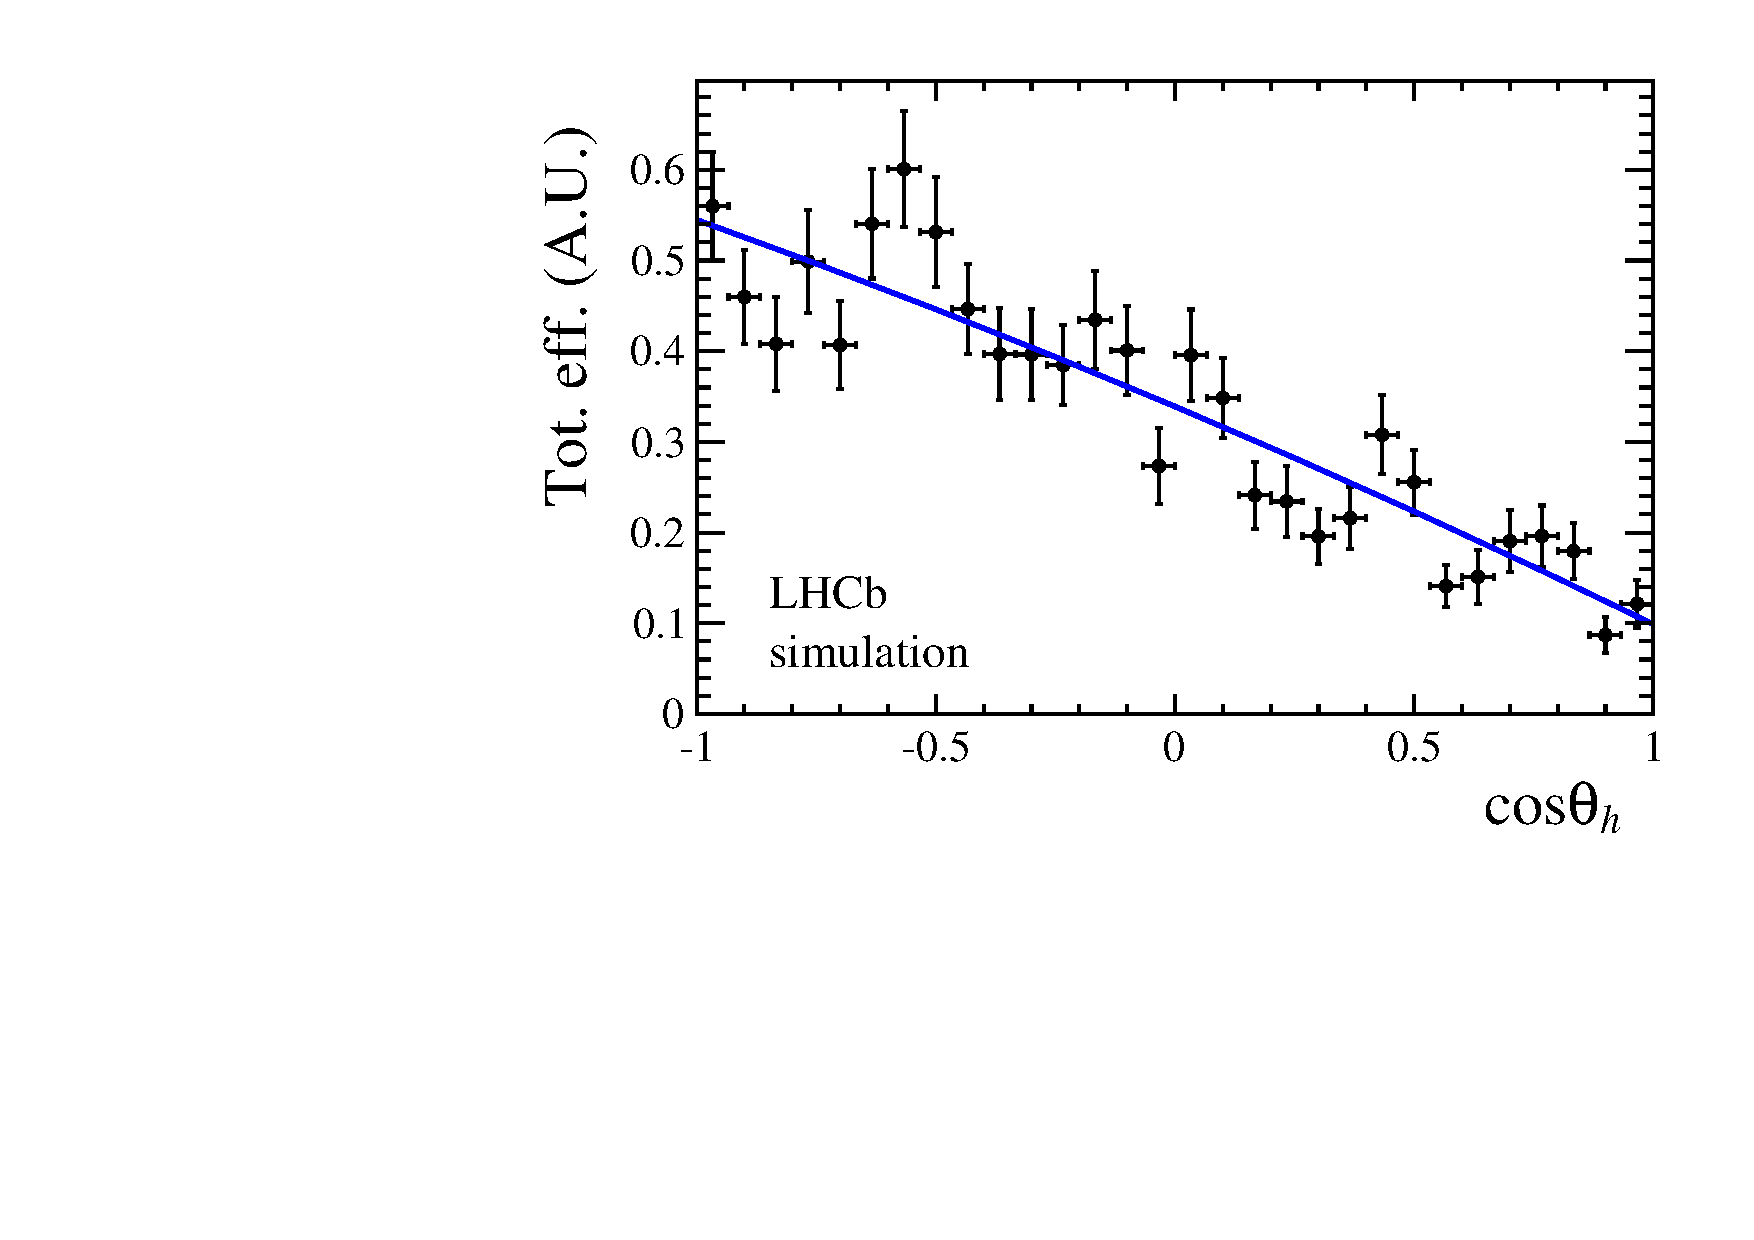
\includegraphics[width=0.45\textwidth]{Lmumu/figs/efficiencies/angular/LLeffFitB_q2_1500_2000.pdf}
\caption{Efficiency as a function of $\cos\theta_\ell$ (top) and $\cos\theta_h$ (bottom) for
downstream (left) and long (right) candidates in the 15--20 \gevgevcccc ~\qsq interval.  }
\label{fig:cosThetaBeff}
\end{figure}
%
\begin{figure}[h]
\centering
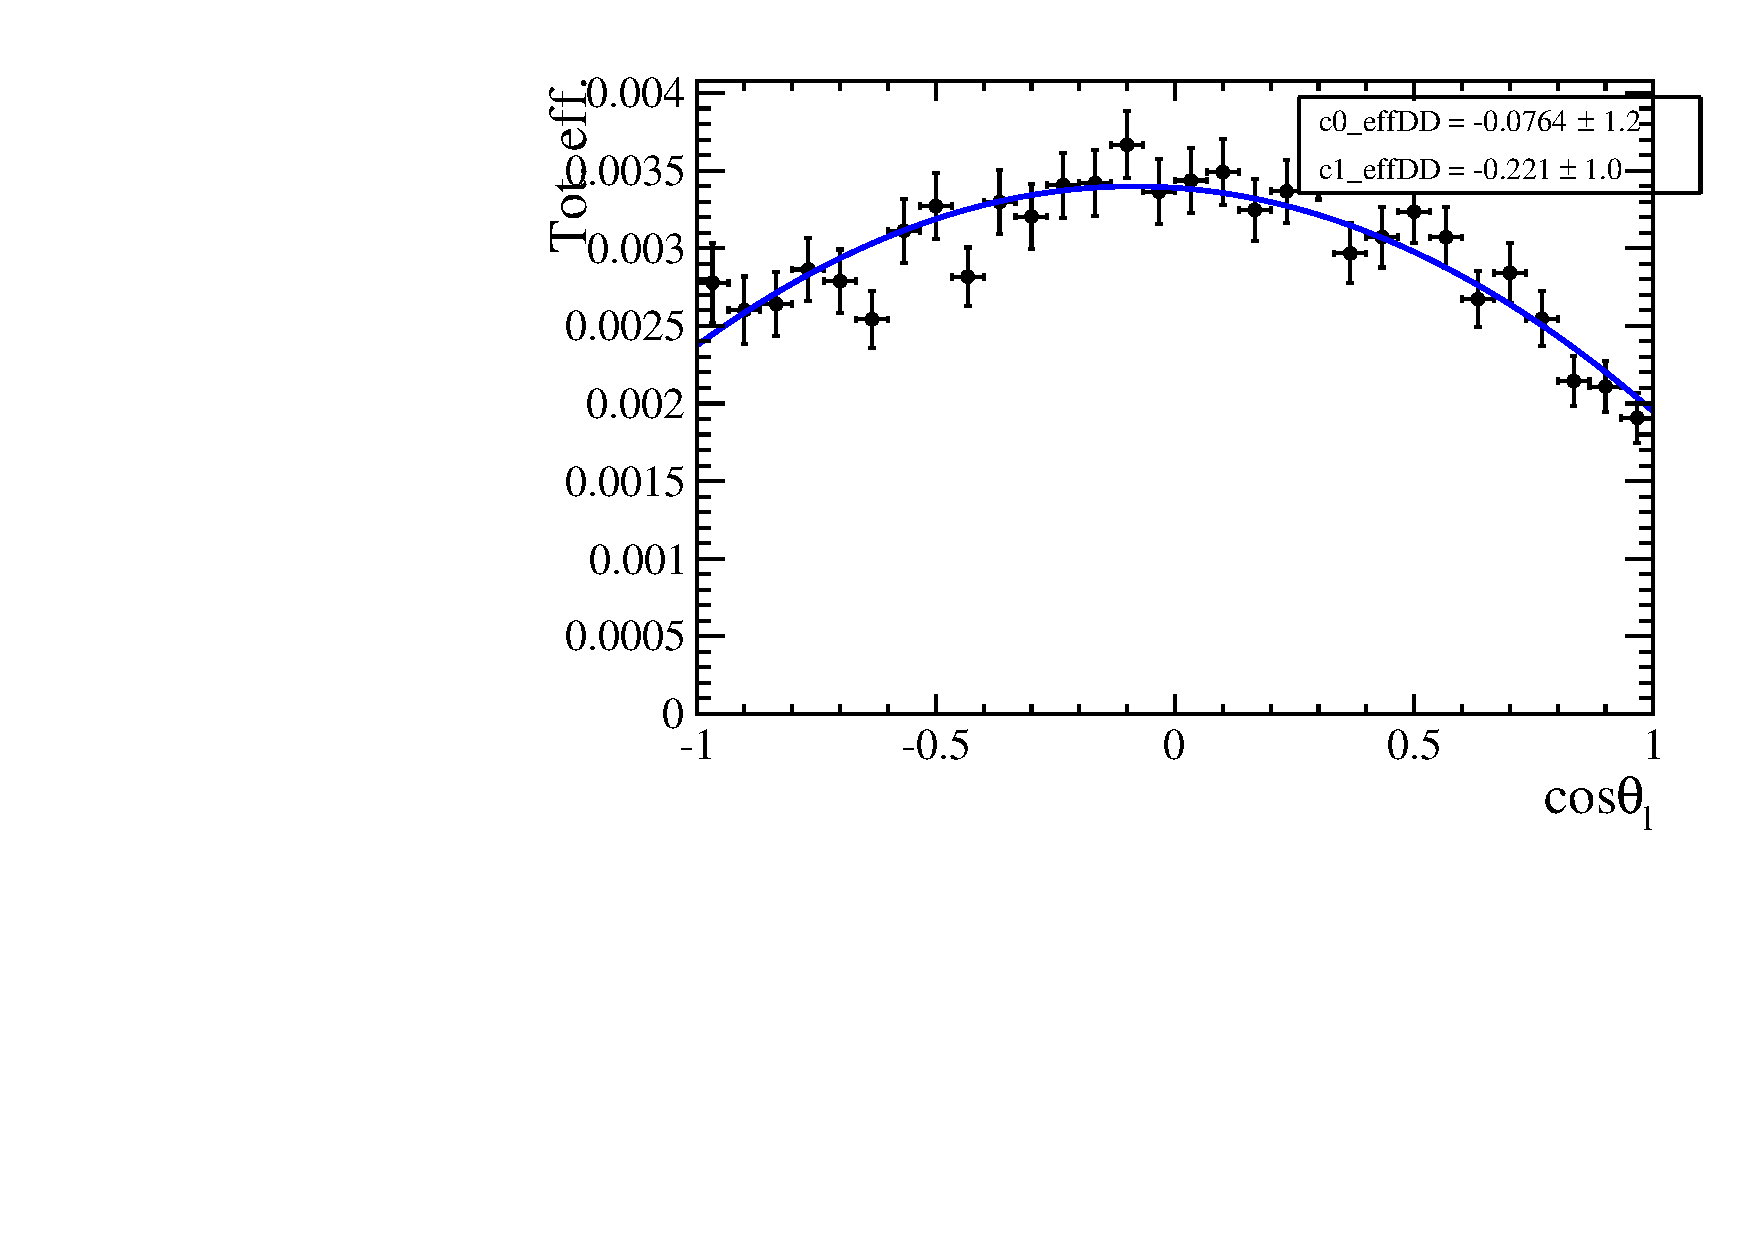
\includegraphics[width=0.45\textwidth]{Lmumu/figs/efficiencies/angular/DDeffFit_q2_110_600.pdf}
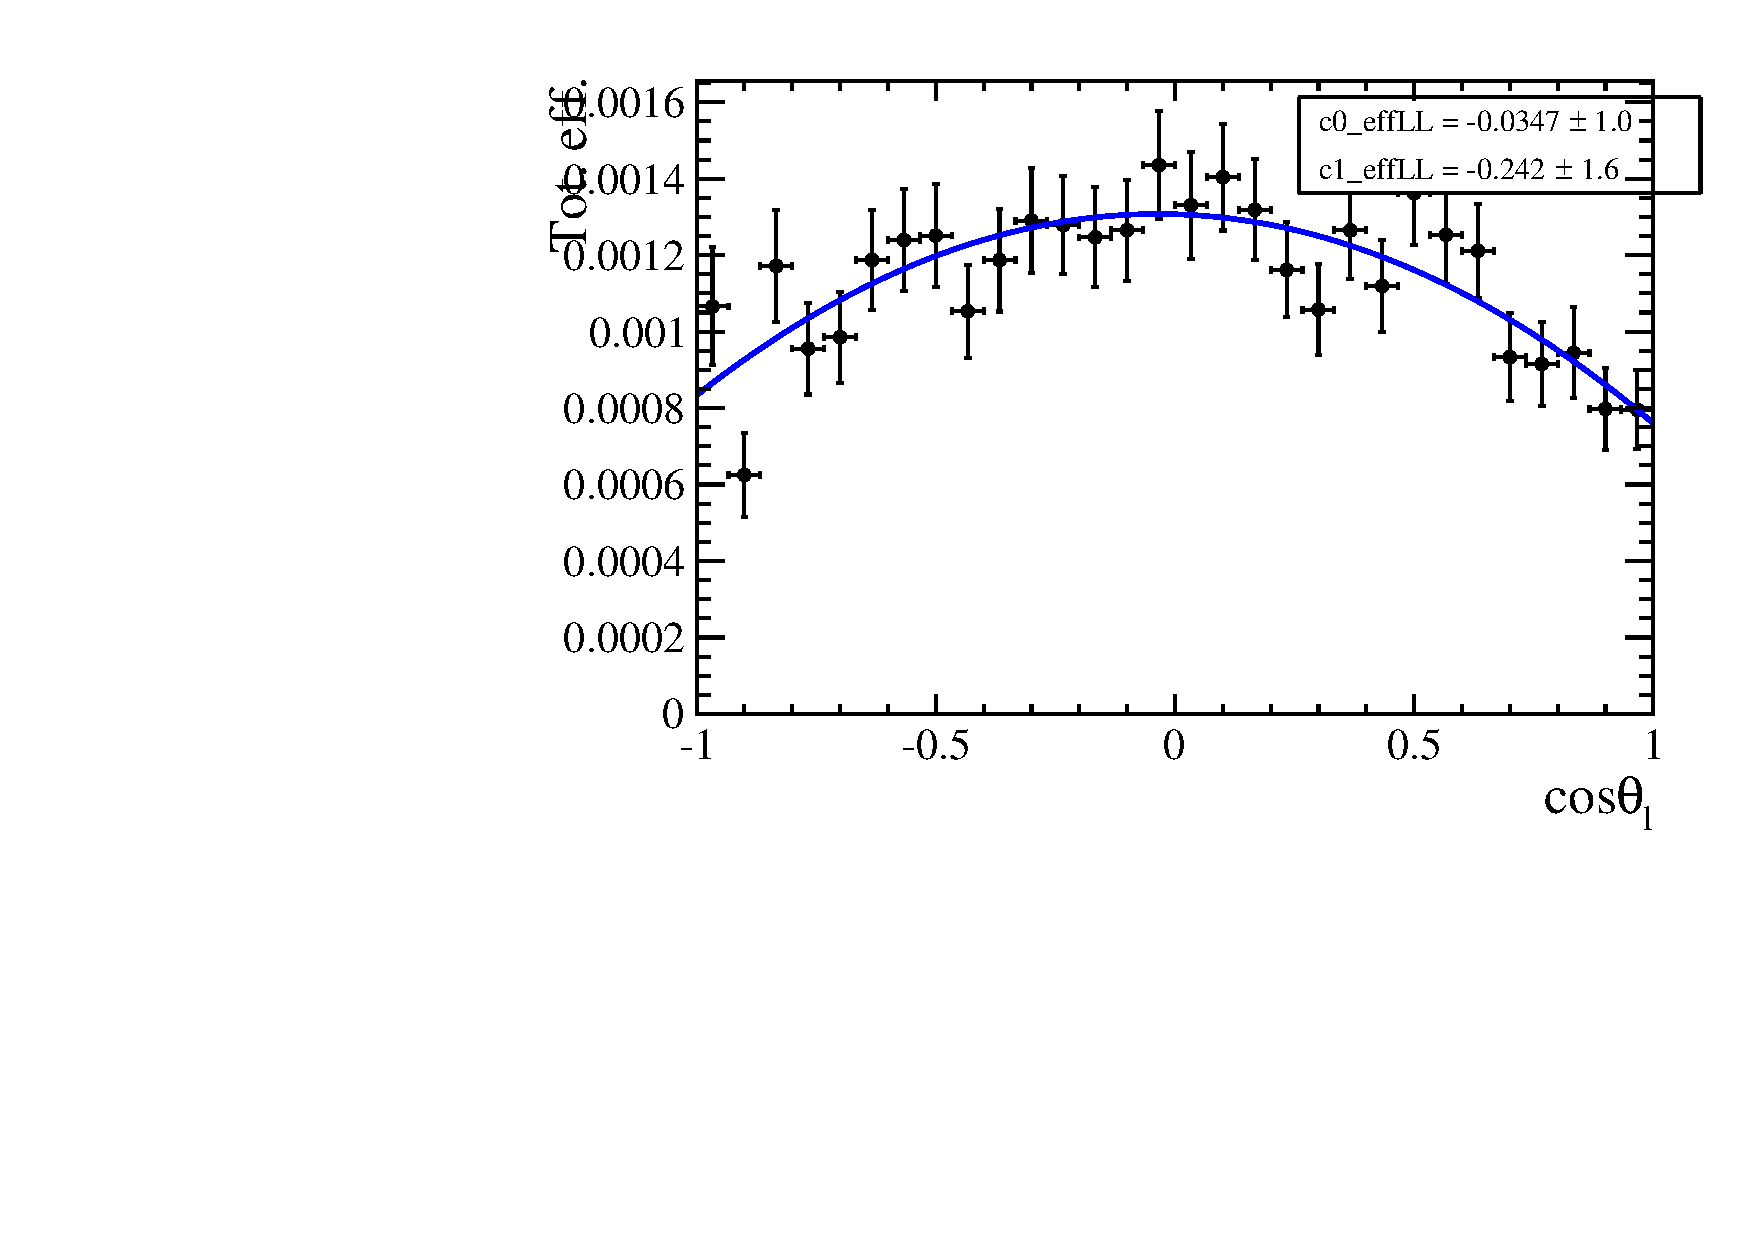
\includegraphics[width=0.45\textwidth]{Lmumu/figs/efficiencies/angular/LLeffFit_q2_110_600.pdf}
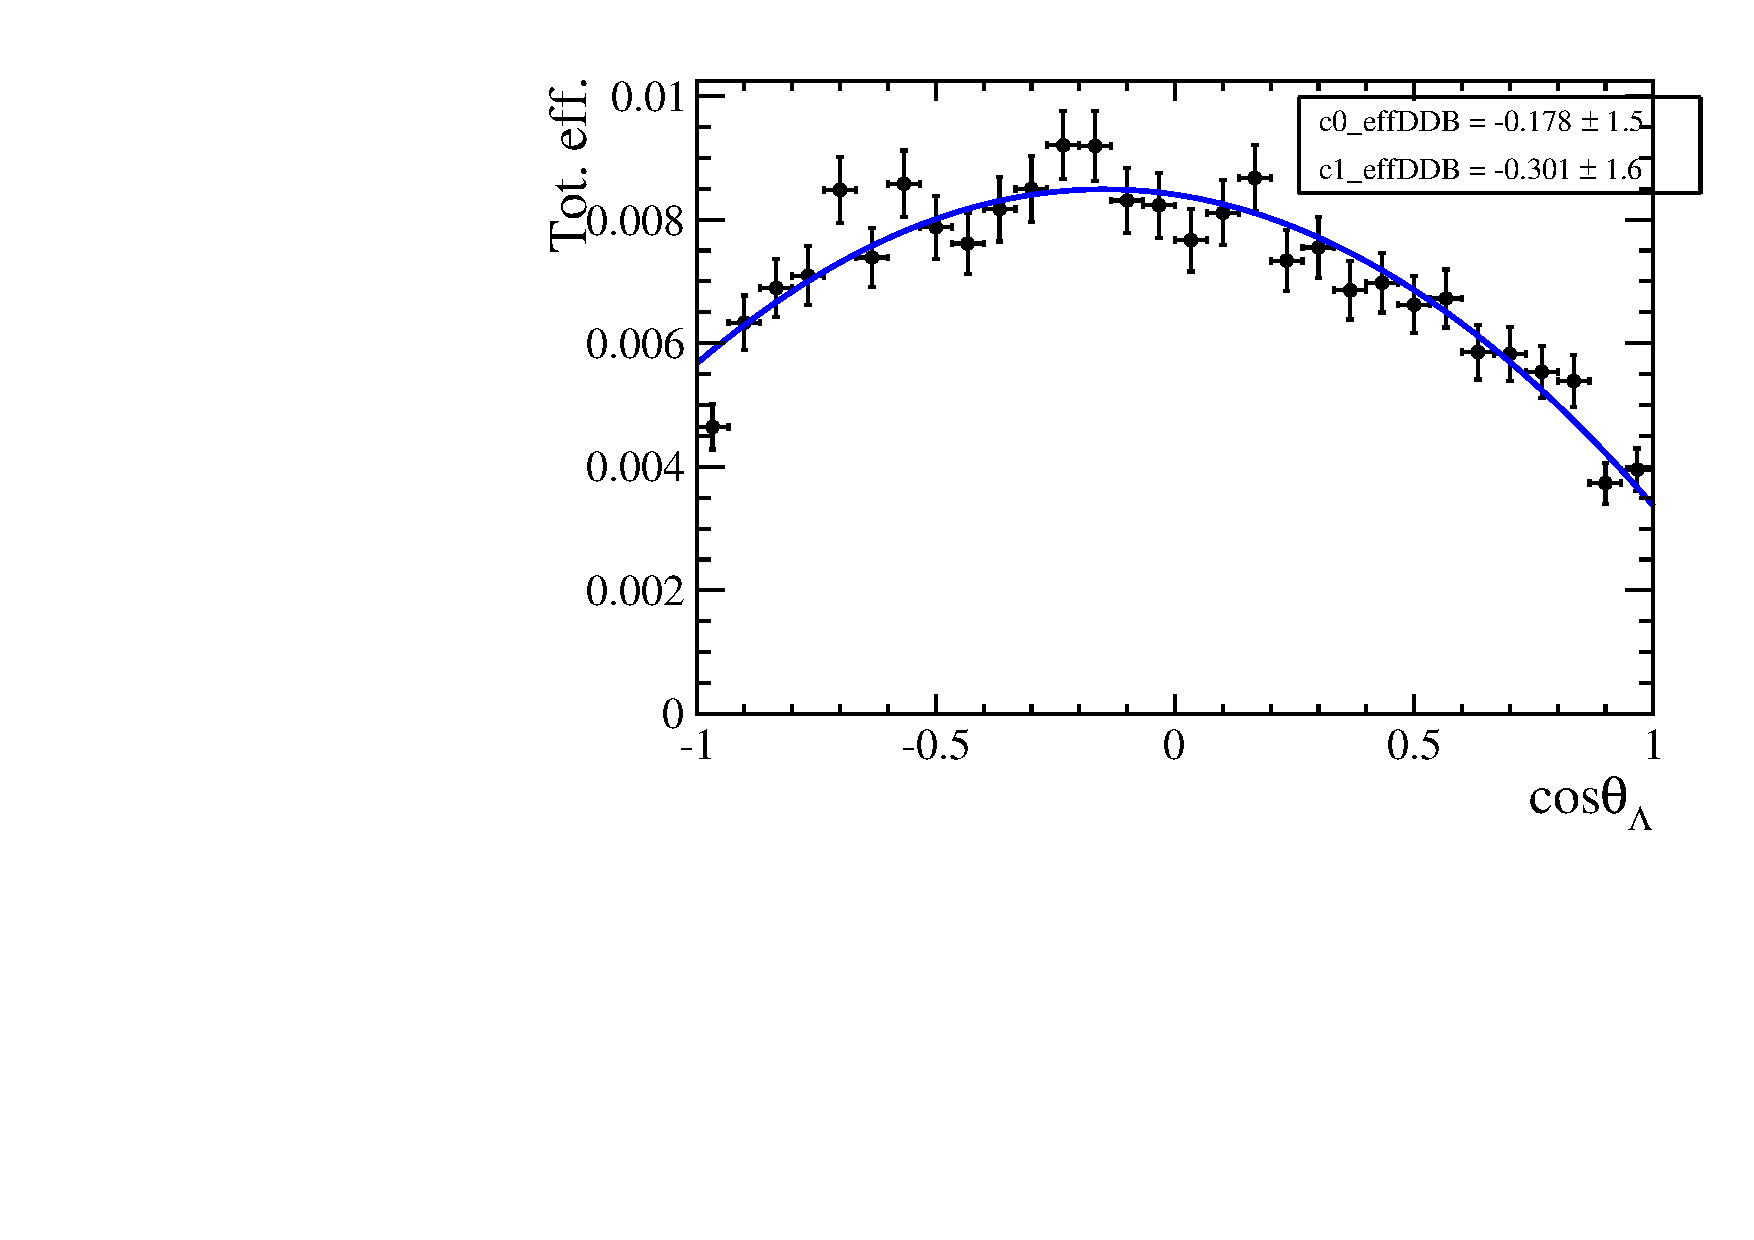
\includegraphics[width=0.45\textwidth]{Lmumu/figs/efficiencies/angular/DDeffFitB_q2_110_600.pdf}
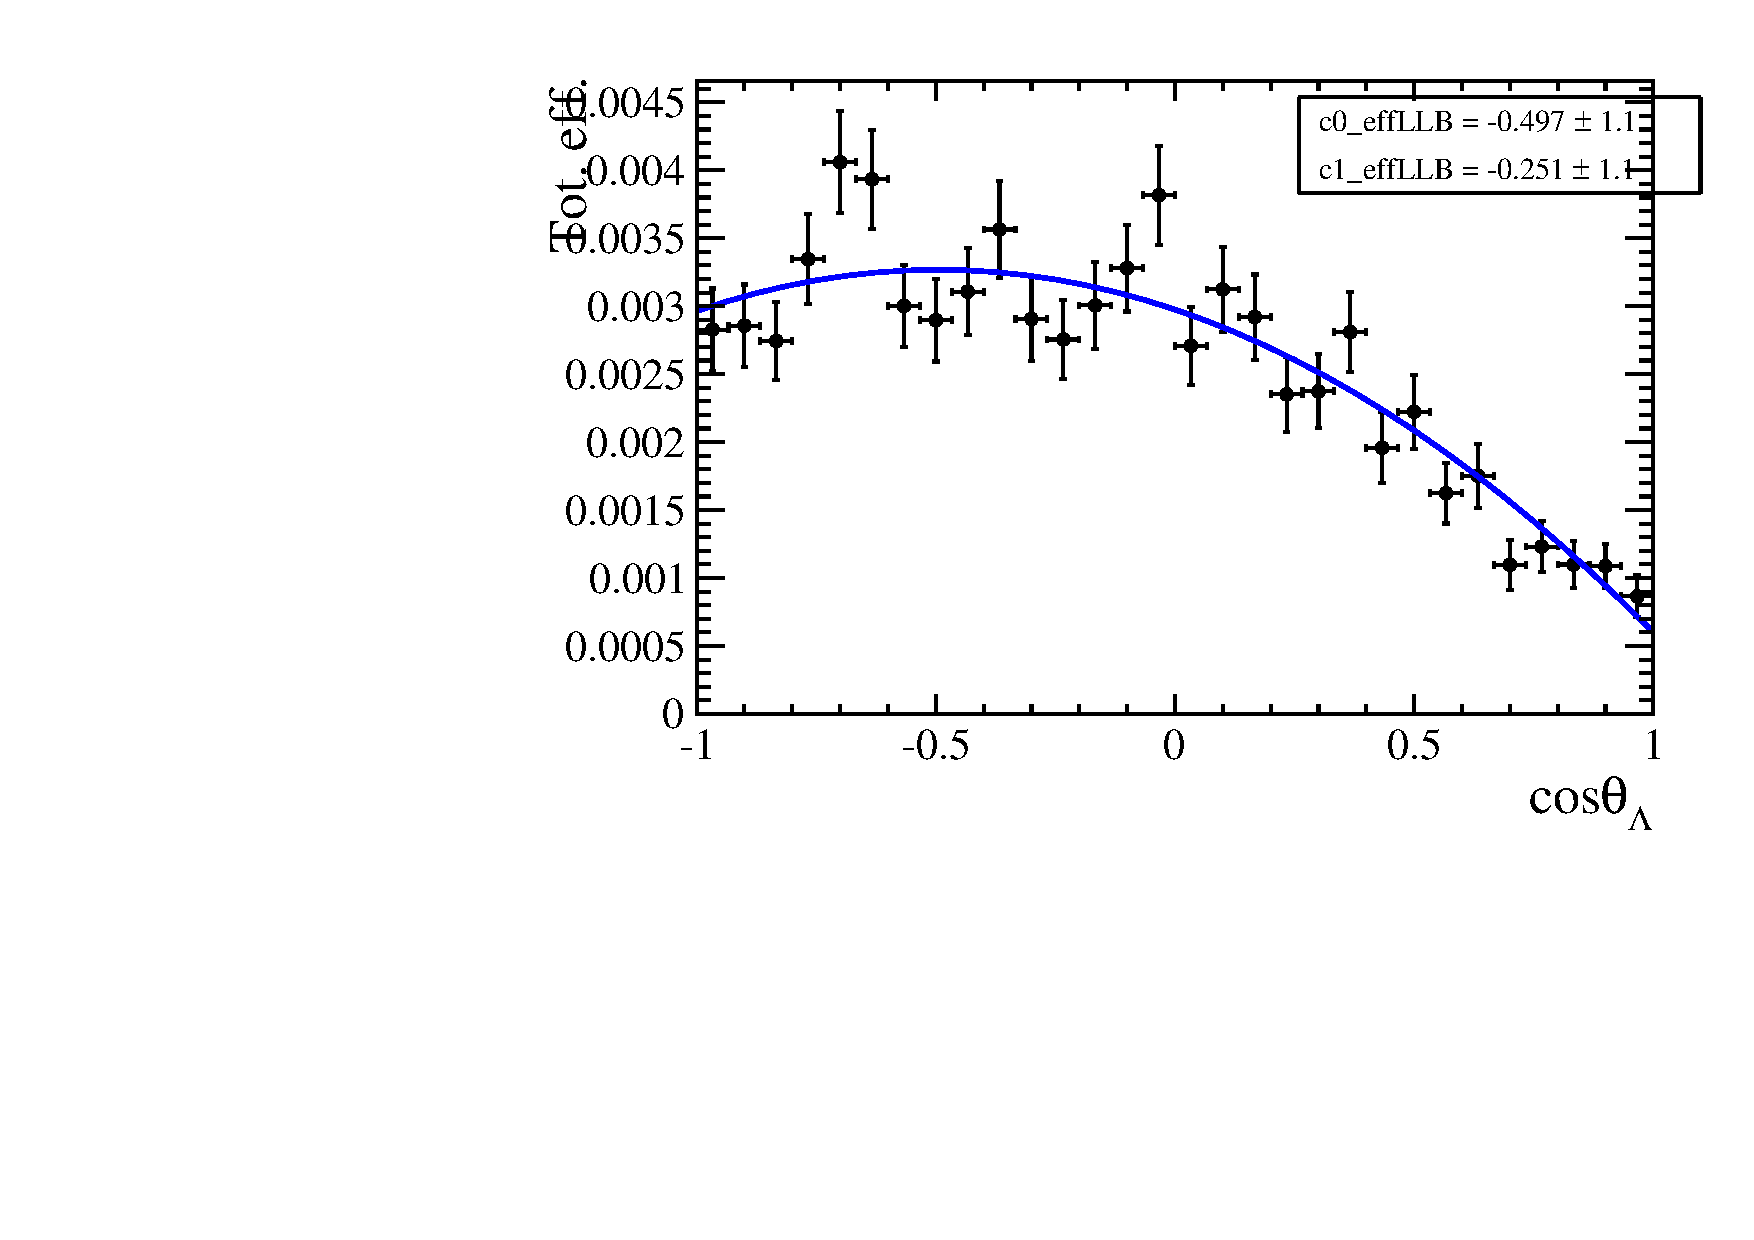
\includegraphics[width=0.45\textwidth]{Lmumu/figs/efficiencies/angular/LLeffFitB_q2_110_600.pdf}
\caption{Efficiency as a function of $\cos\theta_\ell$ (top) and $\cos\theta_h$ (bottom) for
downstream (left) and long (right) candidates in the 1.1--6.0 \gevgevcccc ~\qsq interval.  }
\label{fig:cosThetaBeffLow}
\end{figure}
%
%\begin{figure}[h]
%\centering
%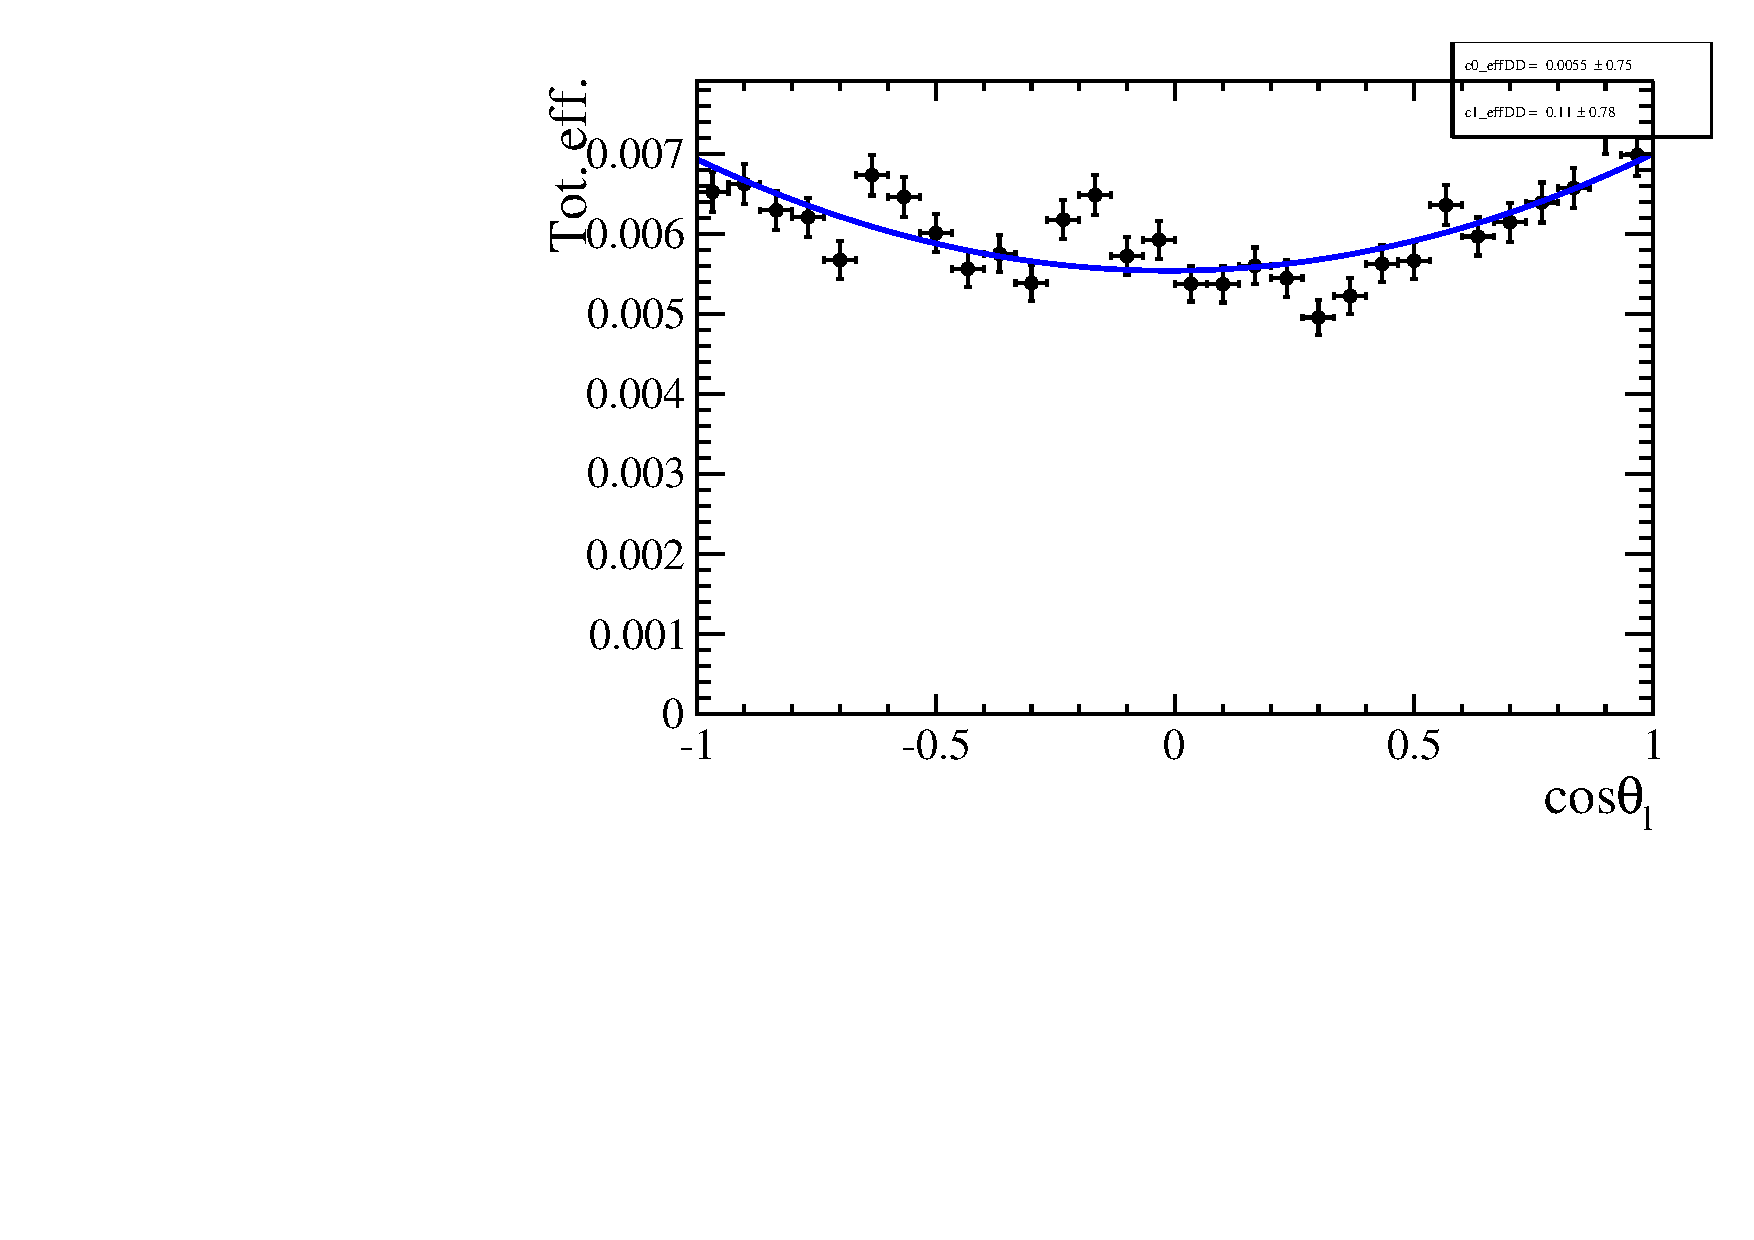
\includegraphics[width=0.45\textwidth]{Lmumu/figs/efficiencies/angular/DDeffFit_jpsi.pdf}
%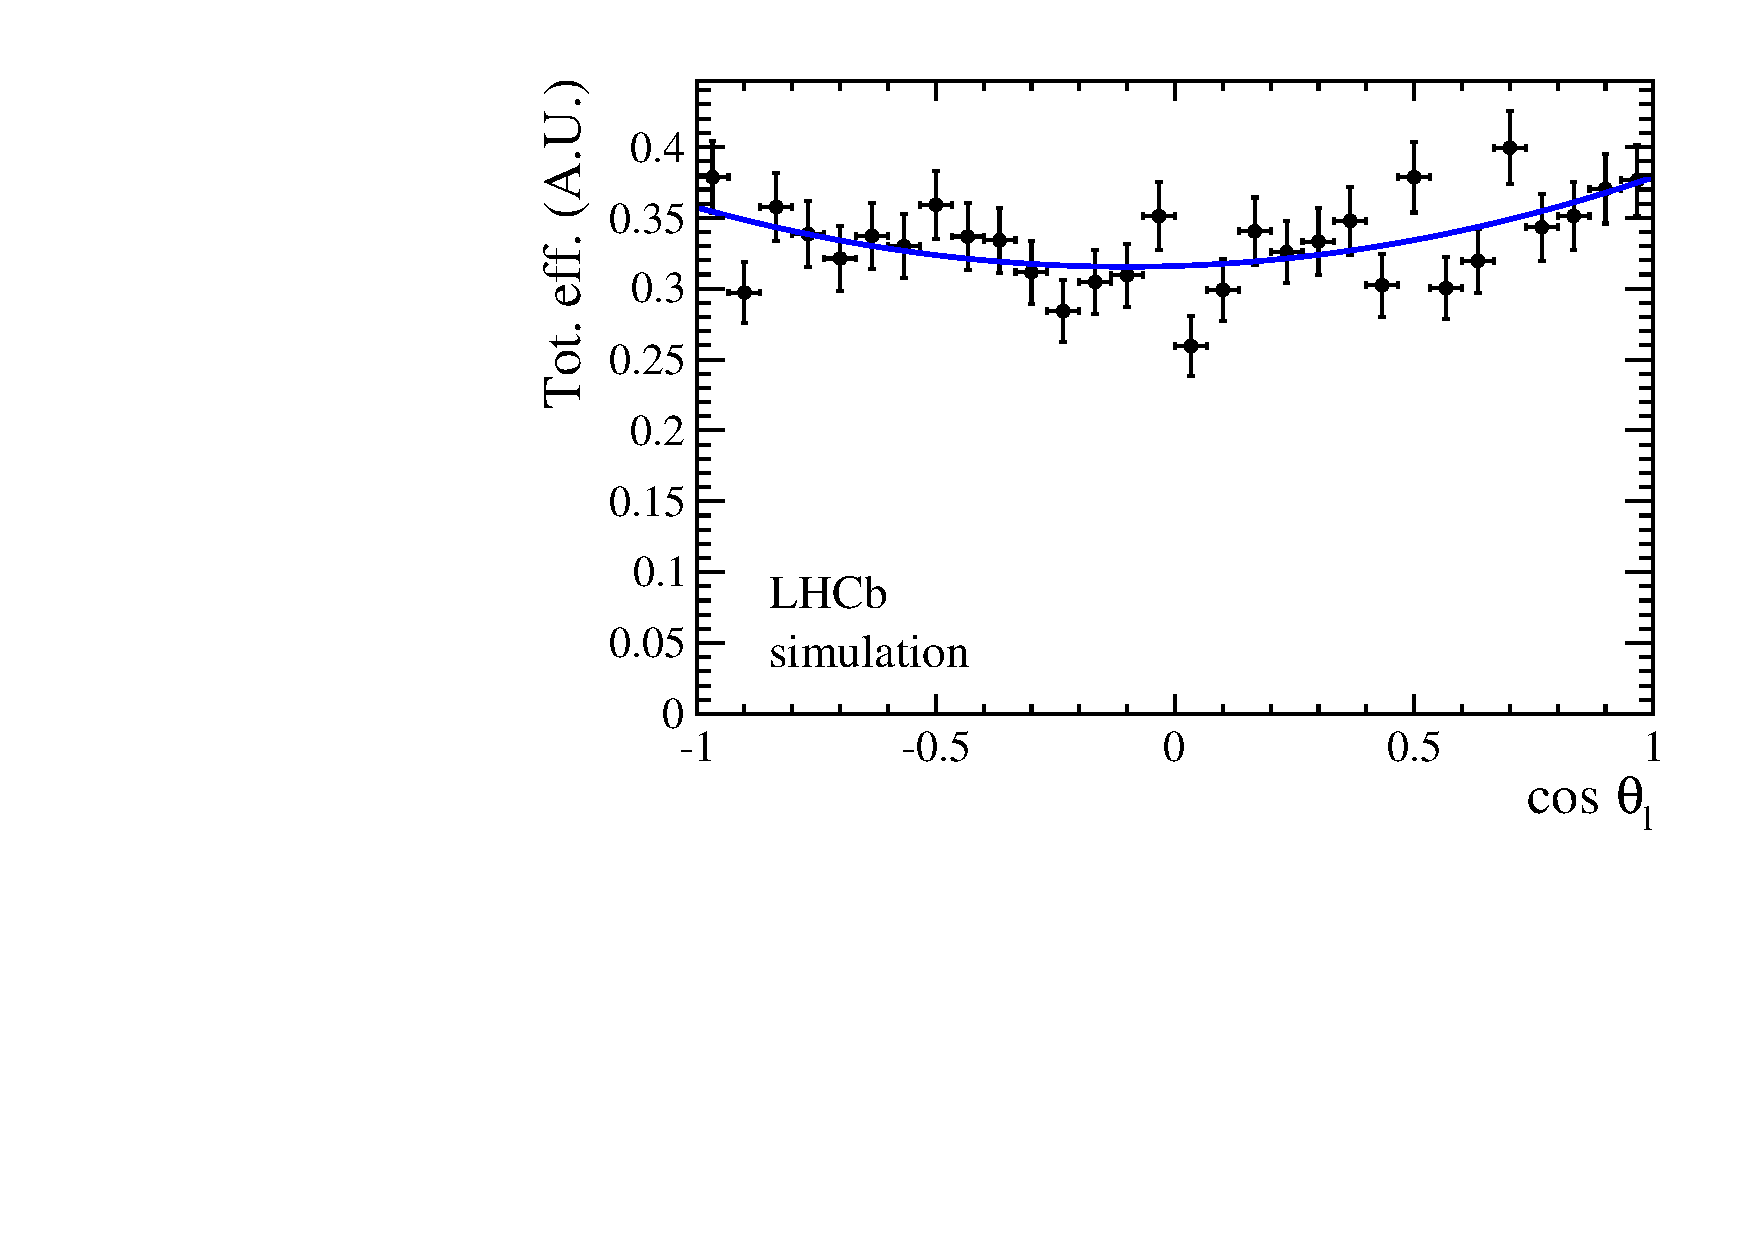
\includegraphics[width=0.45\textwidth]{Lmumu/figs/efficiencies/angular/LLeffFit_jpsi.pdf}
%\caption{Efficiency as a function of $\cos\theta_\ell$ for down-down (left) and long-long (right) events for $J/\psi$ events.  }
%\label{fig:cosThetaLeffJpsi}
%\end{figure}
%
%\begin{figure}[h]
%\centering
%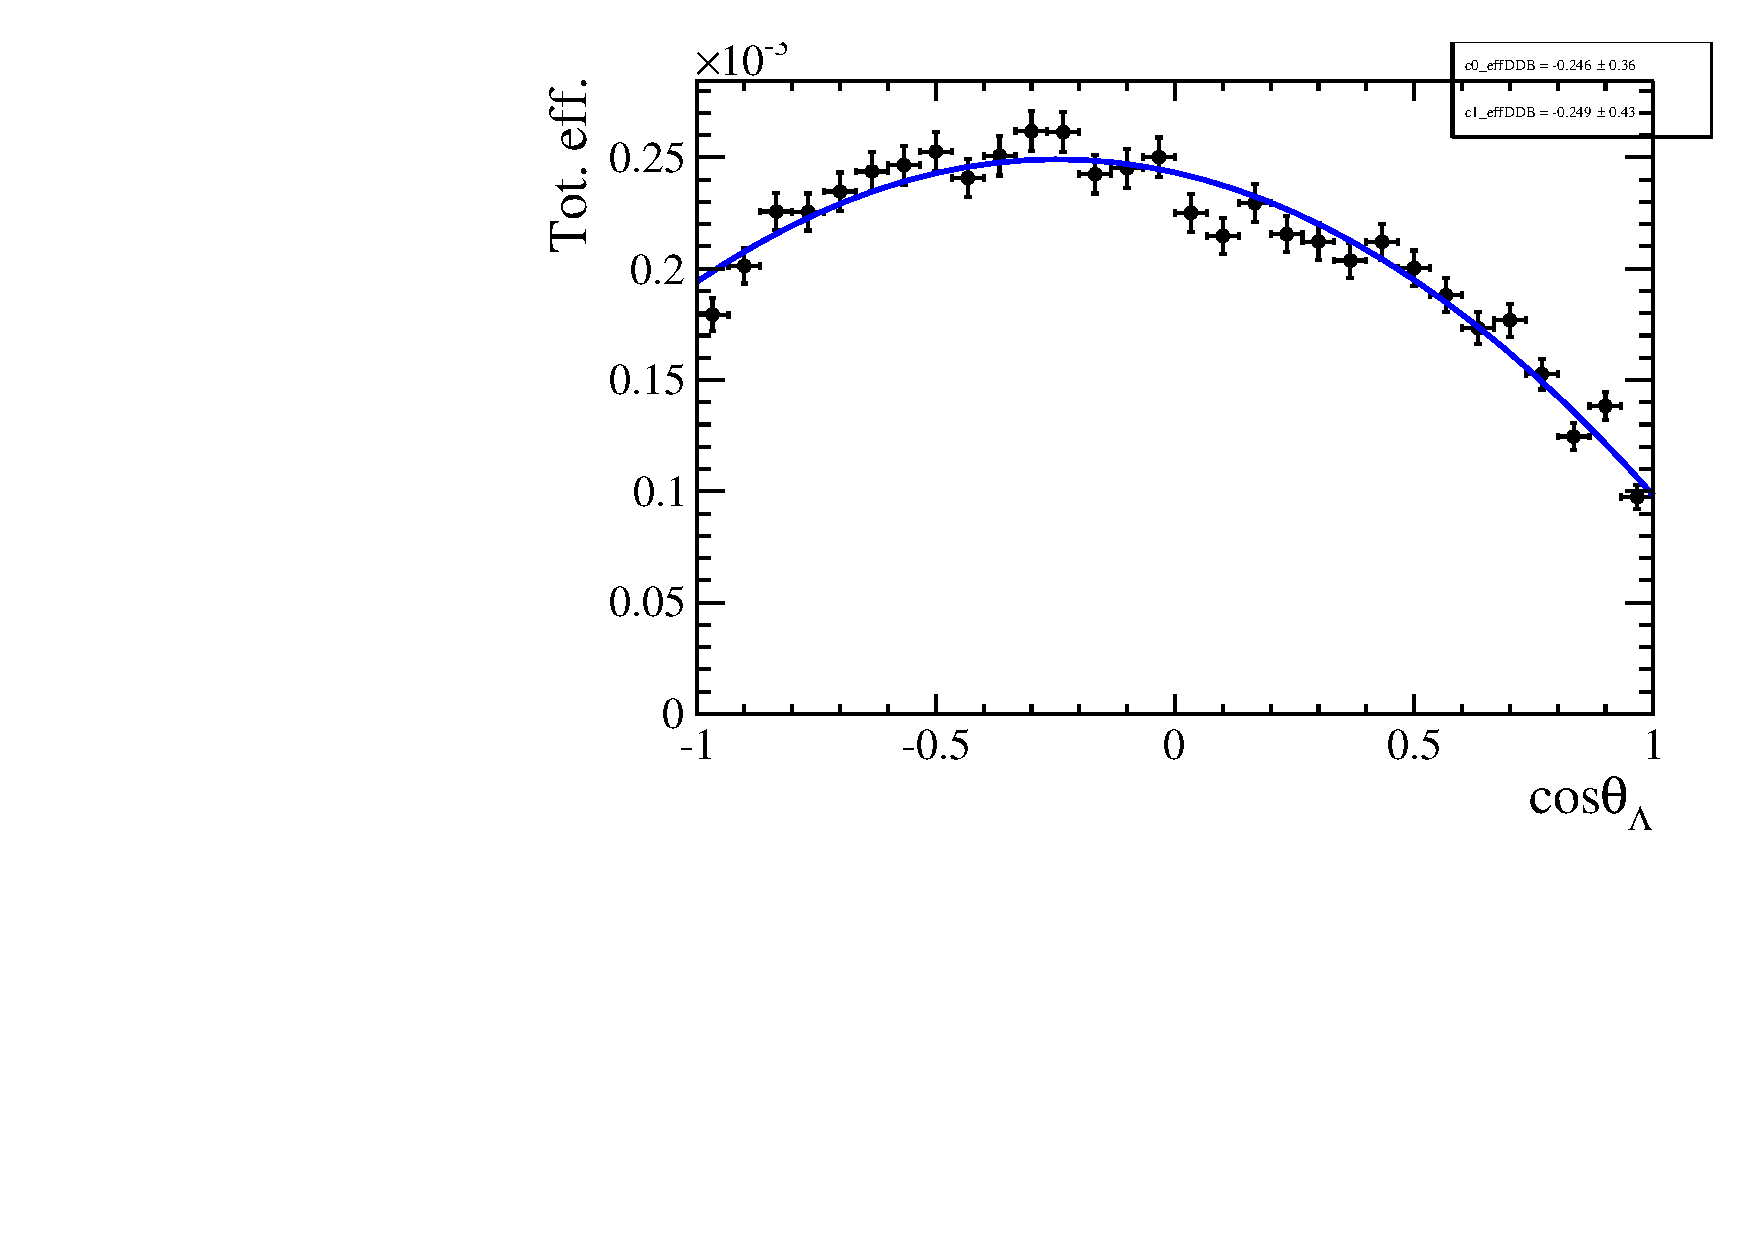
\includegraphics[width=0.45\textwidth]{Lmumu/figs/efficiencies/angular/DDeffFitB_jpsi.pdf}
%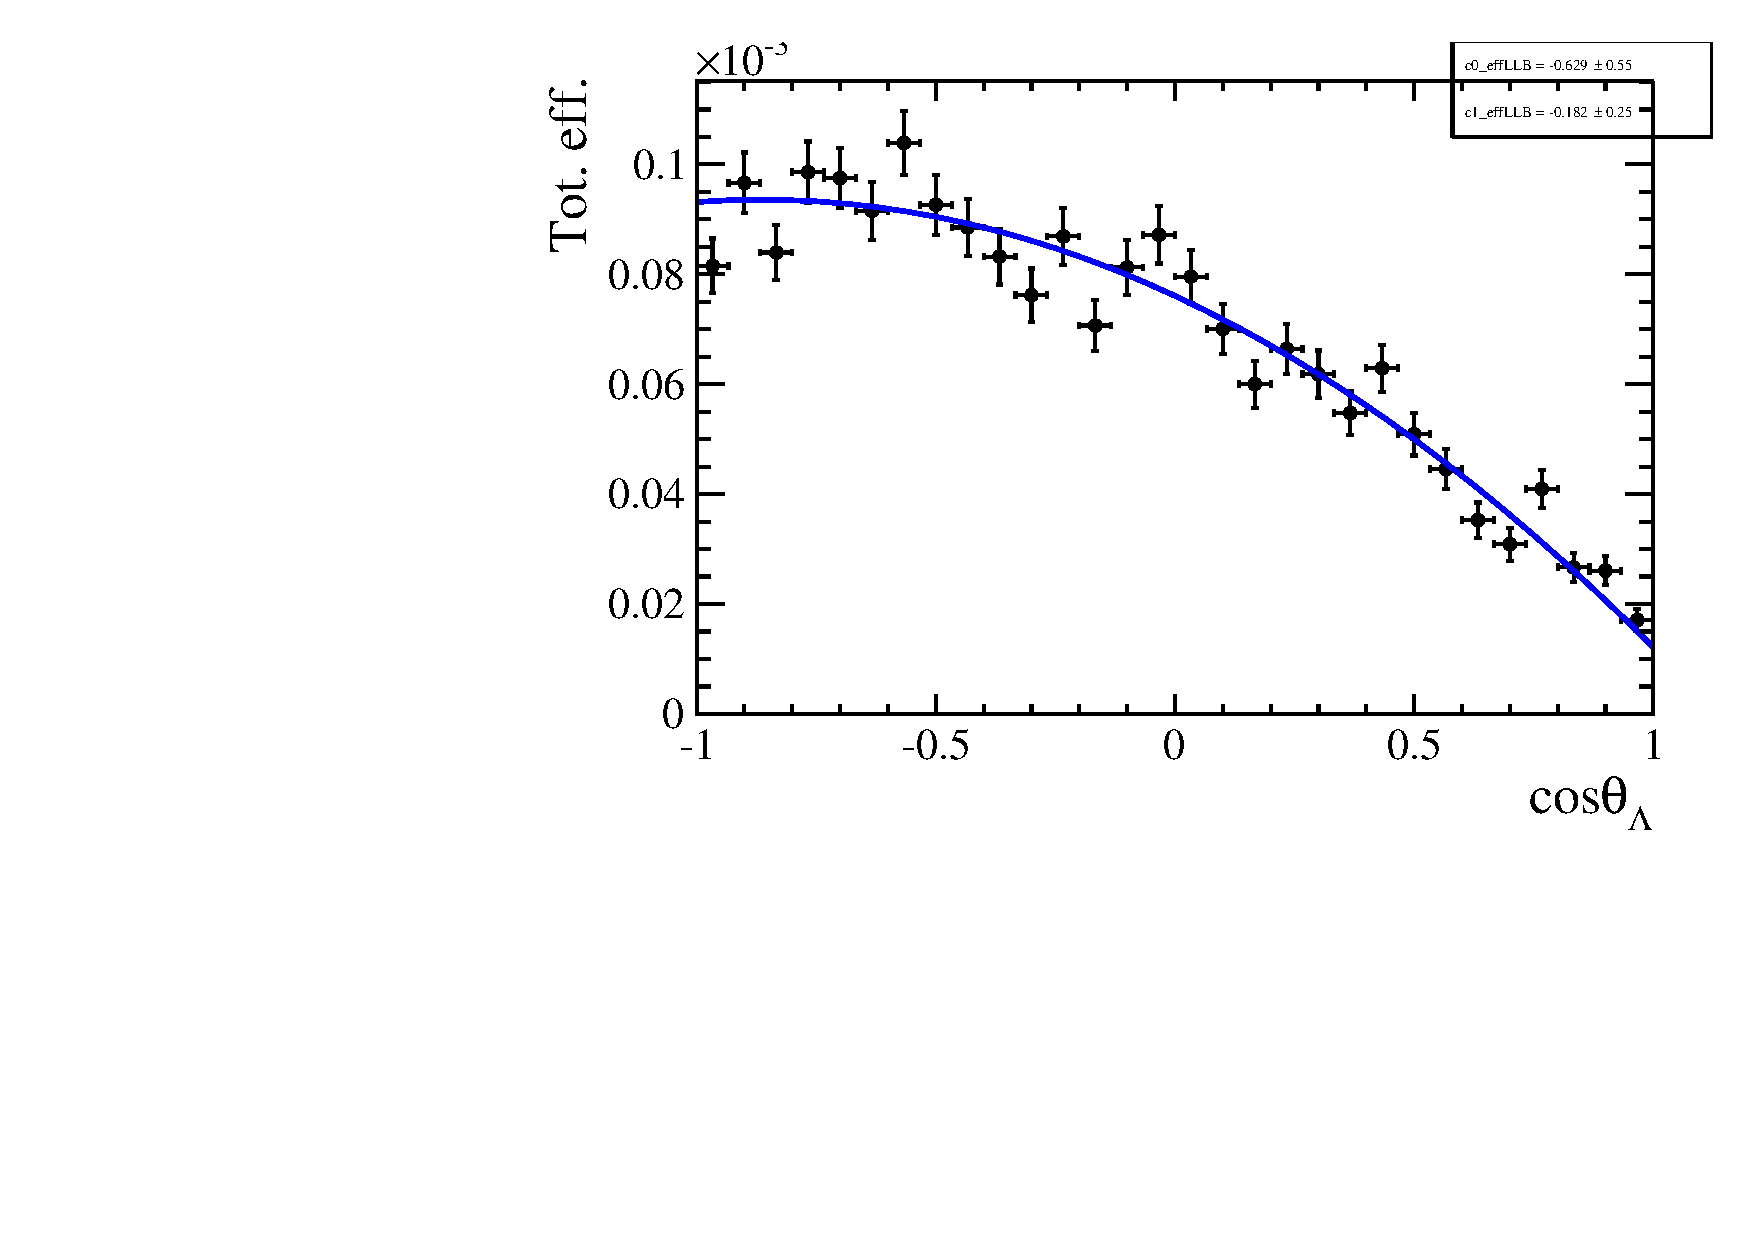
\includegraphics[width=0.45\textwidth]{Lmumu/figs/efficiencies/angular/LLeffFitB_jpsi.pdf}
%\caption{Efficiency as a function of $\cos\theta_\Lambda$ for down-down (left) and long-long (right) events for $J/\psi$ events.  }
%\label{fig:cosThetaBeffJpsi}
%\end{figure}


%Finally, since fits are performed on one-dimensional projections, this implies an integral over
%the other angular variables. If the efficiency is not flat in these variables we could have extra
%terms left in eq. \ref{eq:afbTh} and \ref{eq:afbLTh}. We take in account for this effect in the 
%systematics as described in the following sections. 

\section{Toy studies on a three-dimensional fit}

One other way of extracting the angular observables would be to fit at the same time both angles 
and also the invariant mass distribution in order to have a better handle on the level of background.
In this case one can use more of the information available. On the other hand it is necessary to use 
a larger mass window with more background in it and more parameters to fit.
In the 1D case the free parameters are the two parameters of interest for the lepton case and one
for the hadron one. For the 3D case the free parameters are the three parameters of interest 
plus two background fractions and the two exponential slopes for the invariant mass background.
An high number of free parameters is difficult to constrain with the very limited statistics available.
%Therefore we have a total of 4 free parameters for the lepton case and 3 for hadron case fitting in 1D and 7 free parameters in the 3D fit.
%In both cases we obtain the background fractons fitting mass alone and then we gaussian contrain the fractions in the final fit.
%
To check which method gives the best sensitivity 500 pseudo-experiments are generated.
Events are generated in 3D using shapes taken from the fit on real data.
The generated values of the parameters of interest are $A_{FB}^\ell = 0$, $f_L = 0.7$ 
and $A_{FB}^h = -0.37$. These are data-like values inspired to what is measured in the highest
statistics interval. The overall statistics and the fraction of bacgkround events in the mass
window are constrained to what obtained from the fit on real data.
%This is done using the statistics of our highest statistics bin, $15-20$ $GeV^2/c^2$ in \qsq, 
%and our lowest statistics unblinded bin, $11-12.5$ $GeV^2/c^2$ in \qsq.
Each pseudo-experiment is fitted with both methods and Fig.~\ref{fig:3DtoyResults} reports 
distributions of parameters of interest obtained from the fit in the 1D and 3D cases.
The RMS of these distributions can be taken as a measure of the sensitivity of each method.
In Tab.~\ref{tab:3DtoyResults} RMSs from both methods can be compared. For all parameters 
of interest the 1D fit method gives a smaller RMS, hence a better sensitivity.

\begin{figure}[h]
\centering
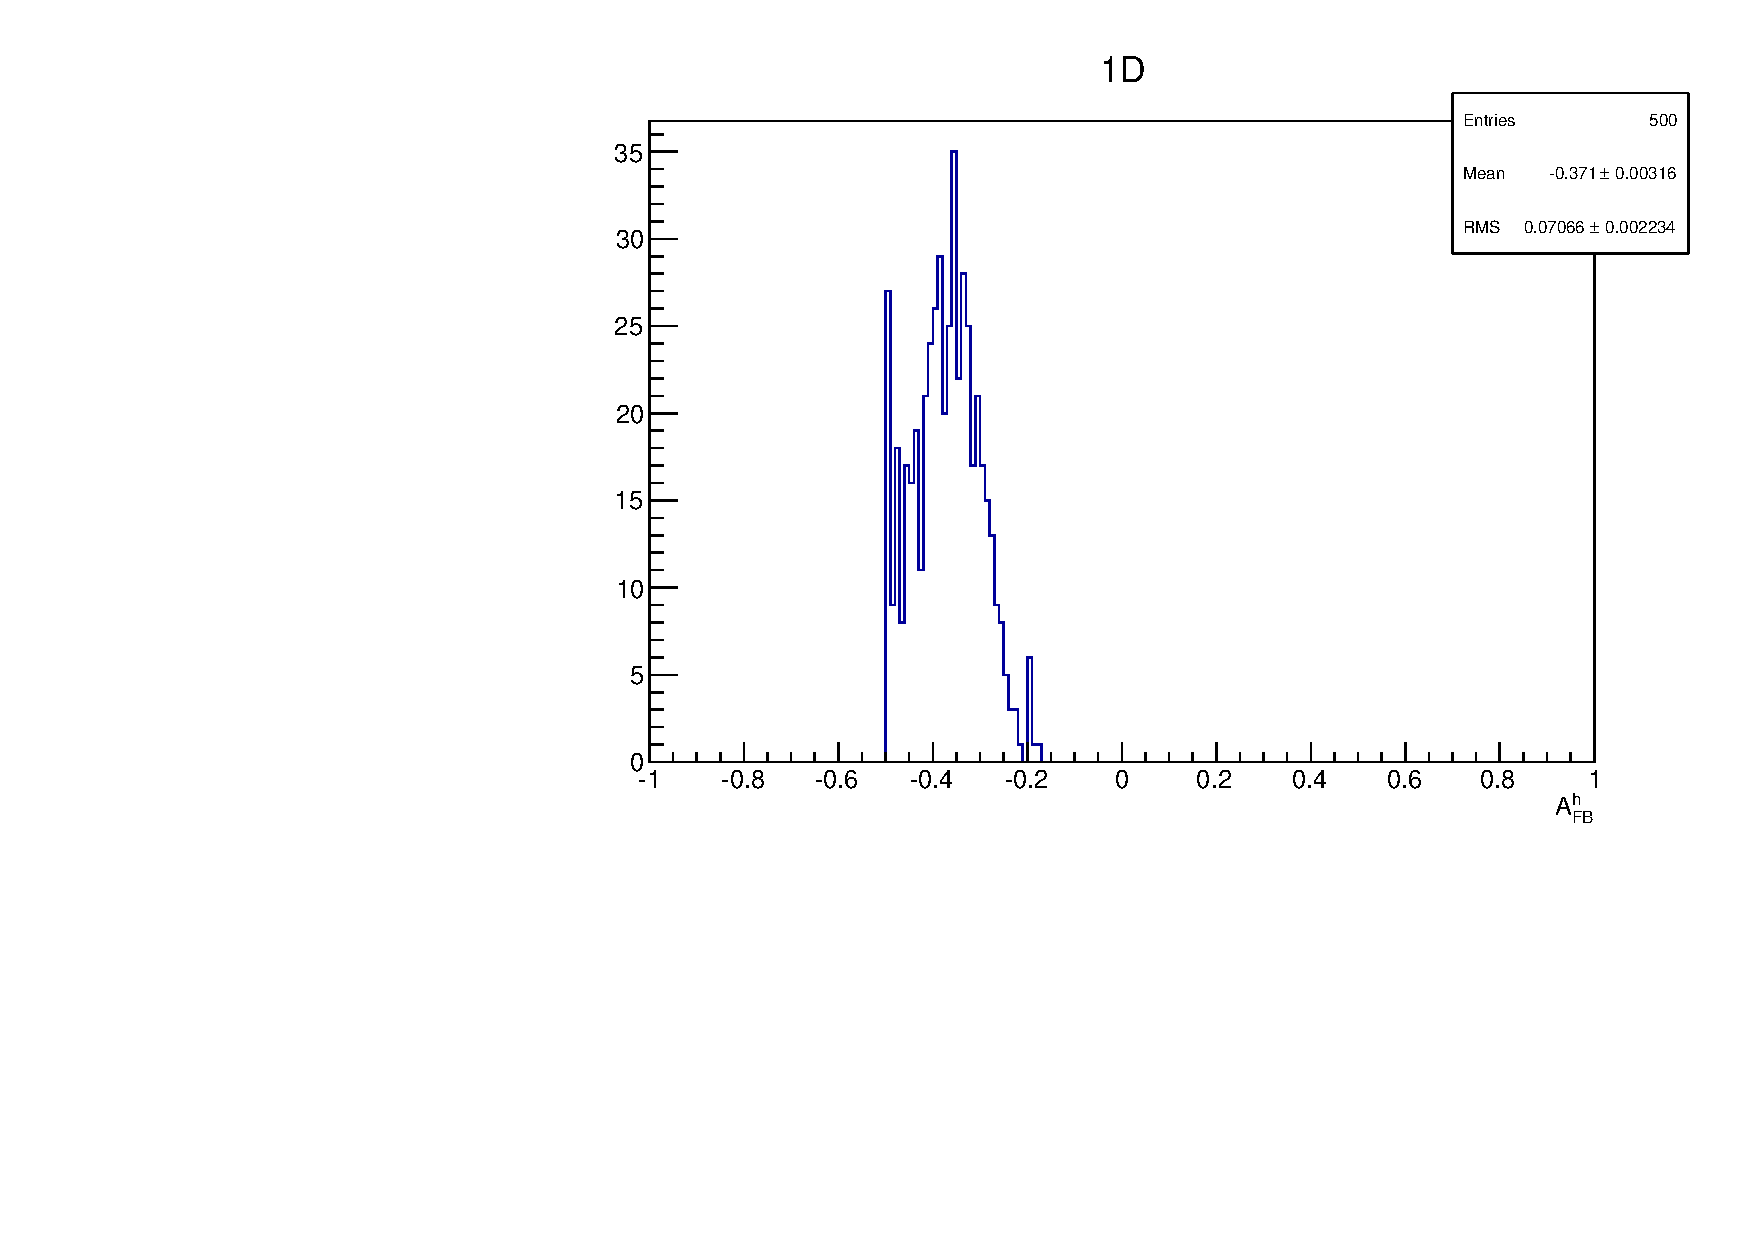
\includegraphics[width=0.3\textwidth]{Lmumu/figs/toys3D/B1/1D/toys3D_afbB.pdf}
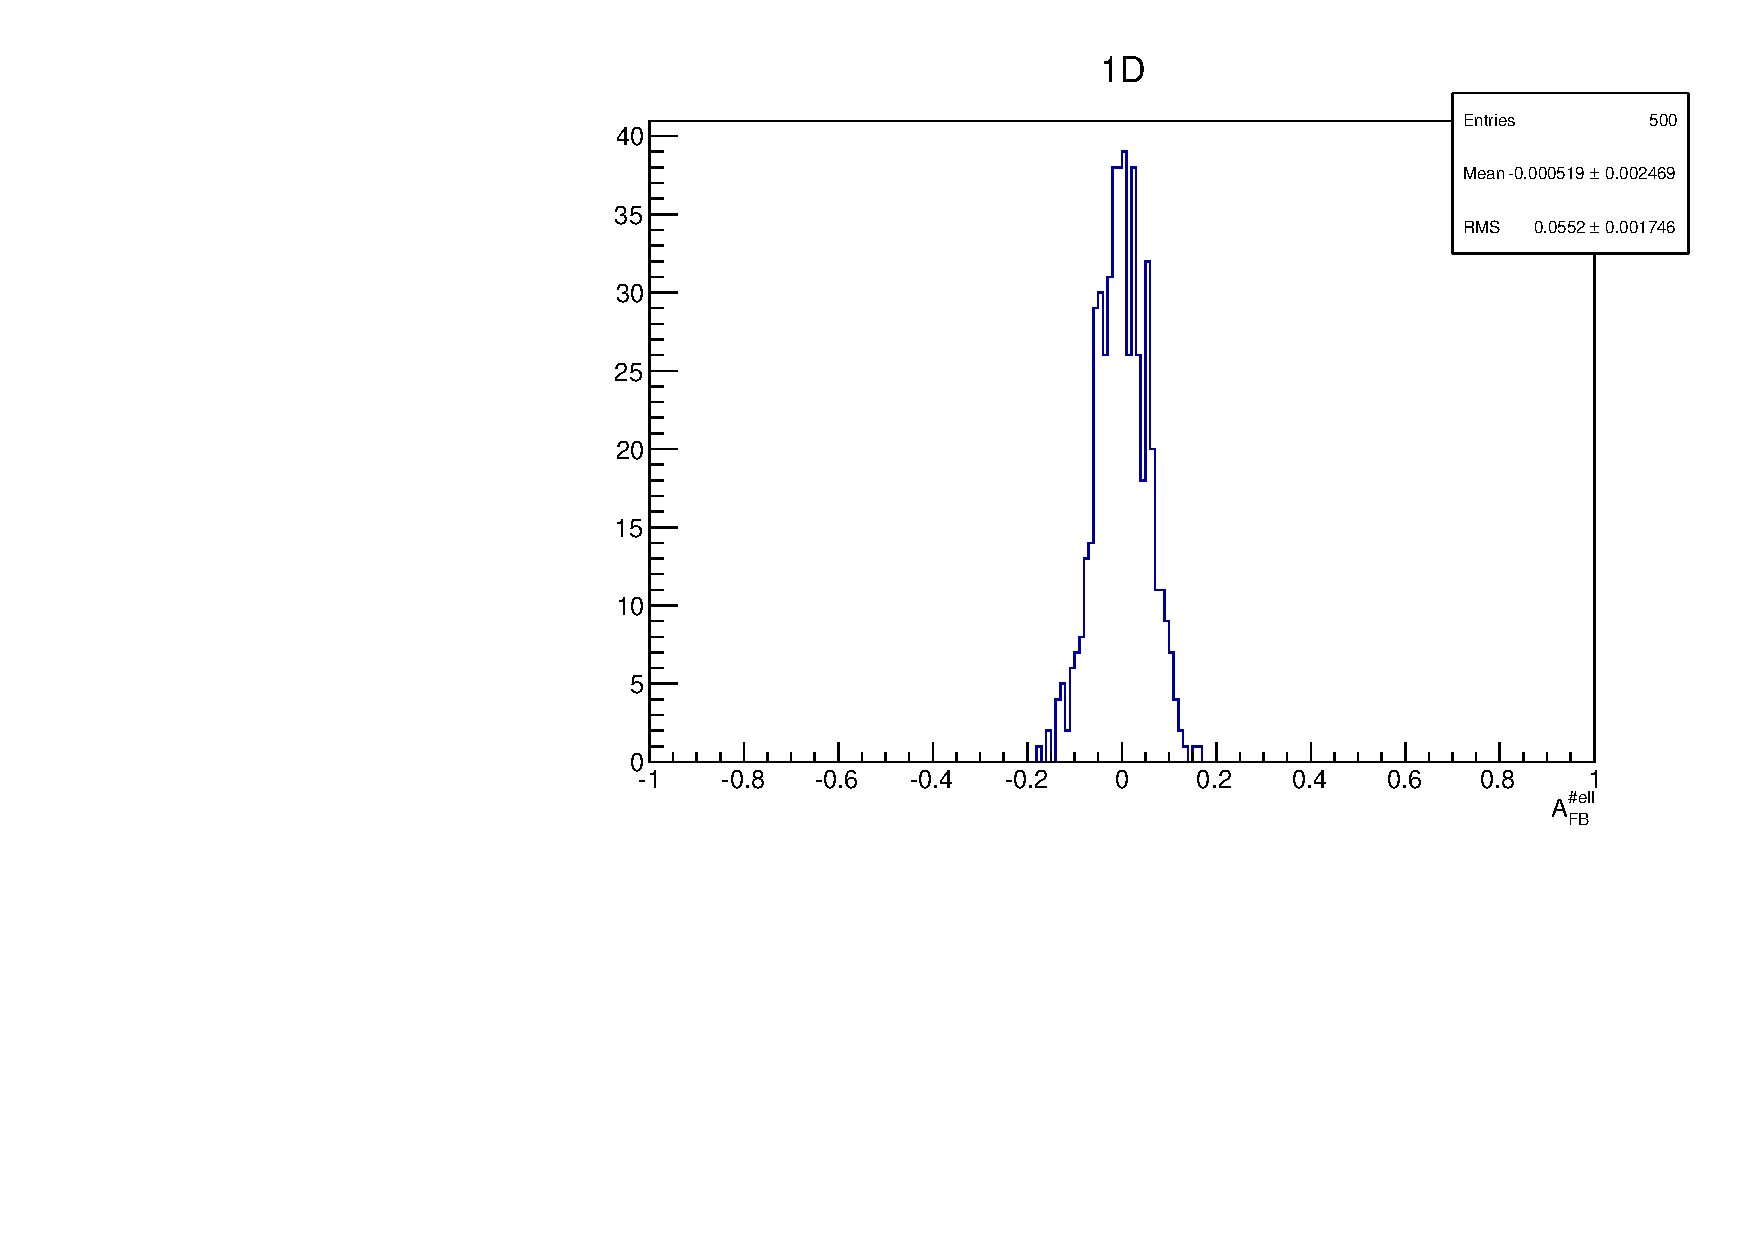
\includegraphics[width=0.3\textwidth]{Lmumu/figs/toys3D/B1/1D/toys3D_afb.pdf}
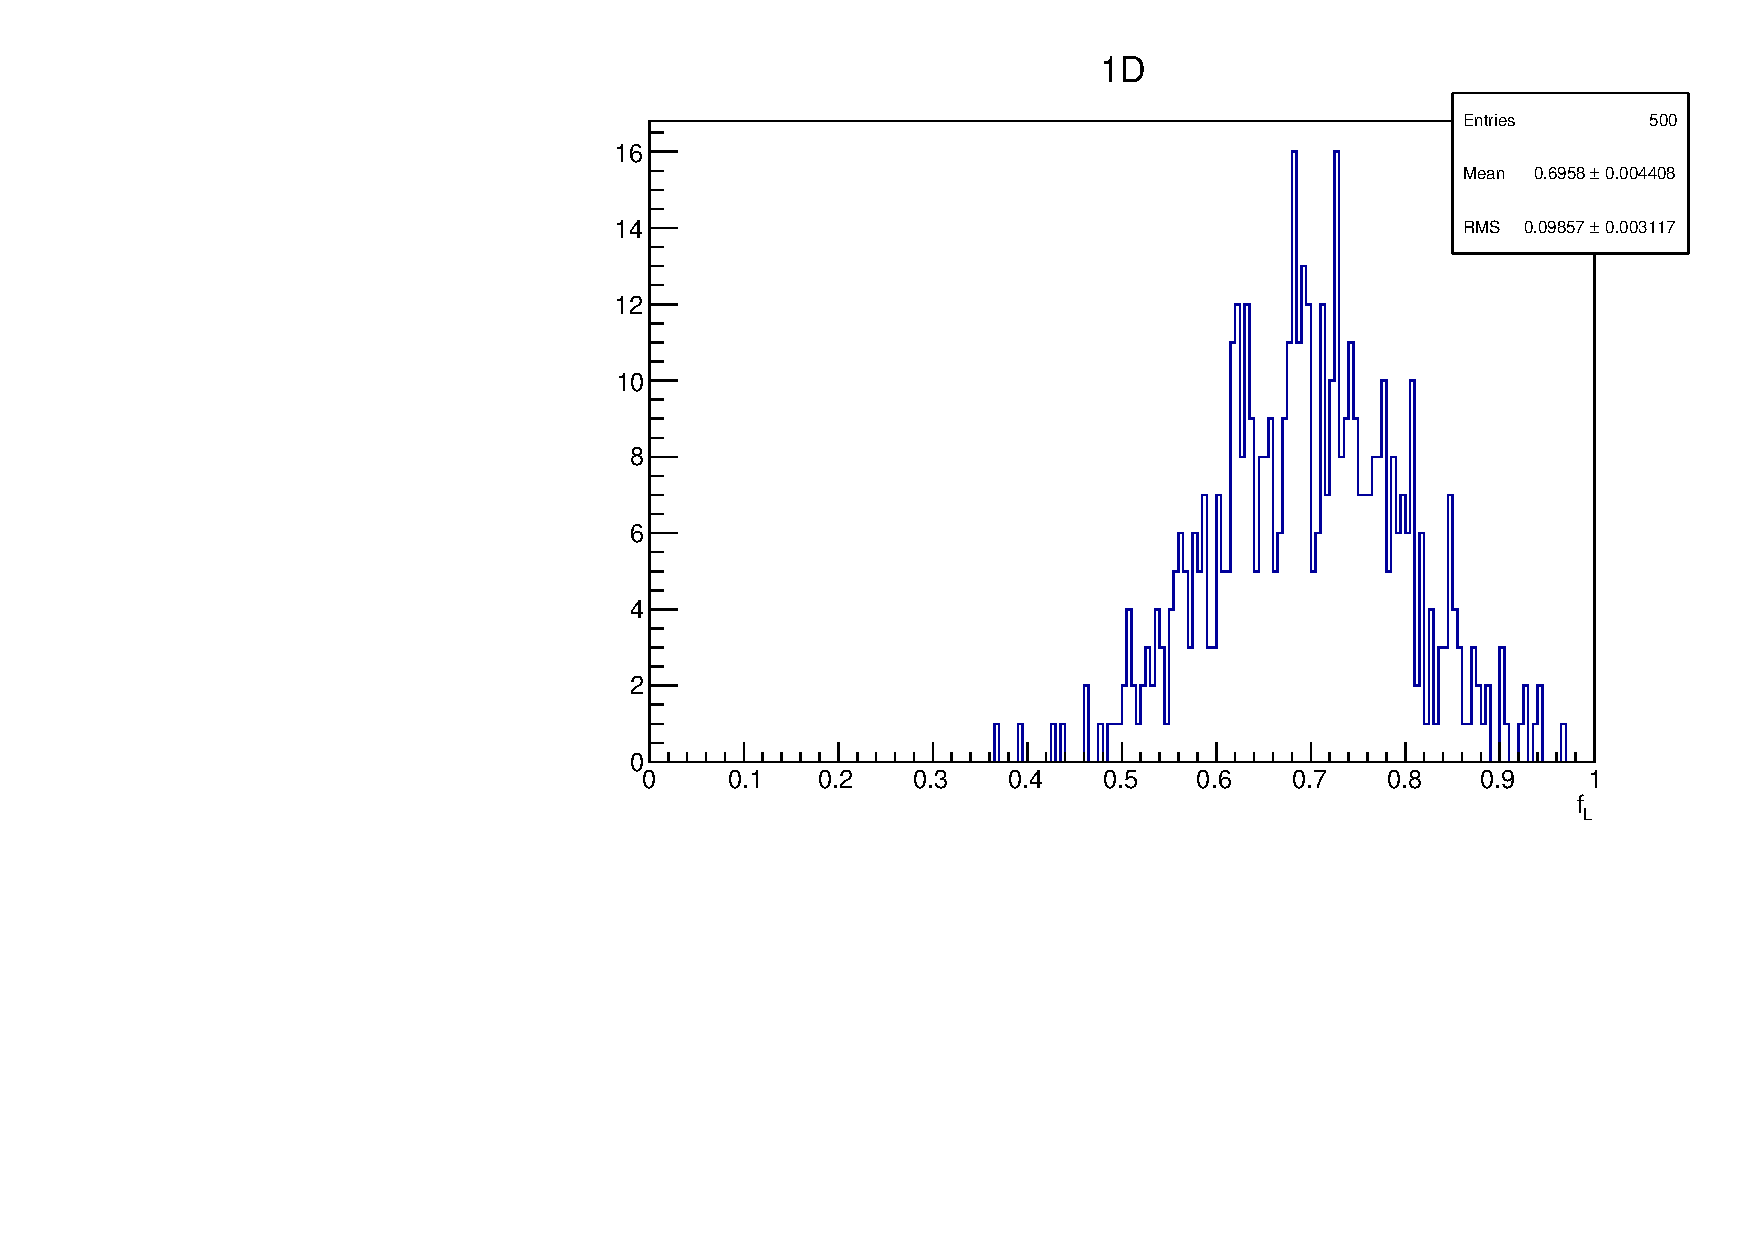
\includegraphics[width=0.3\textwidth]{Lmumu/figs/toys3D/B1/1D/toys3D_fL.pdf} \\
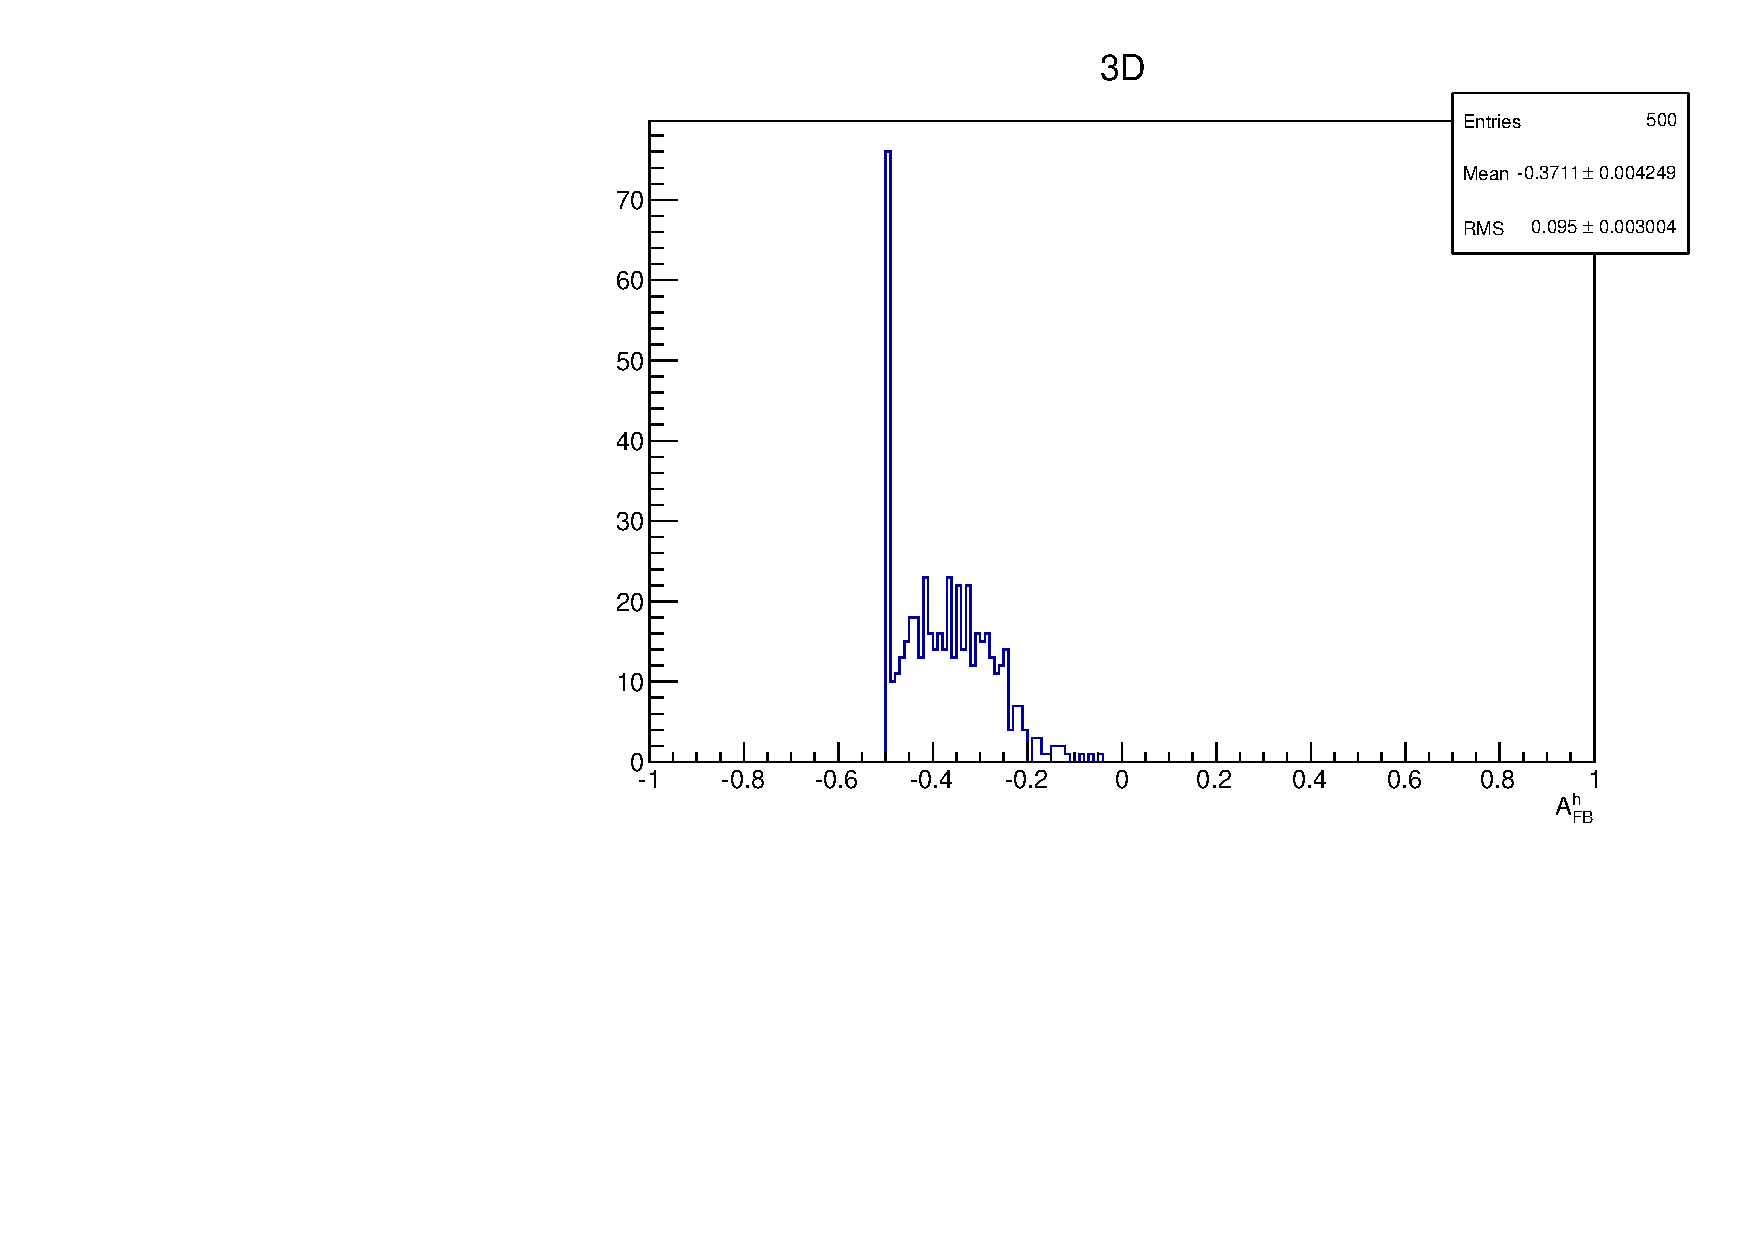
\includegraphics[width=0.3\textwidth]{Lmumu/figs/toys3D/B1/3D/toys3D_afbB.pdf}
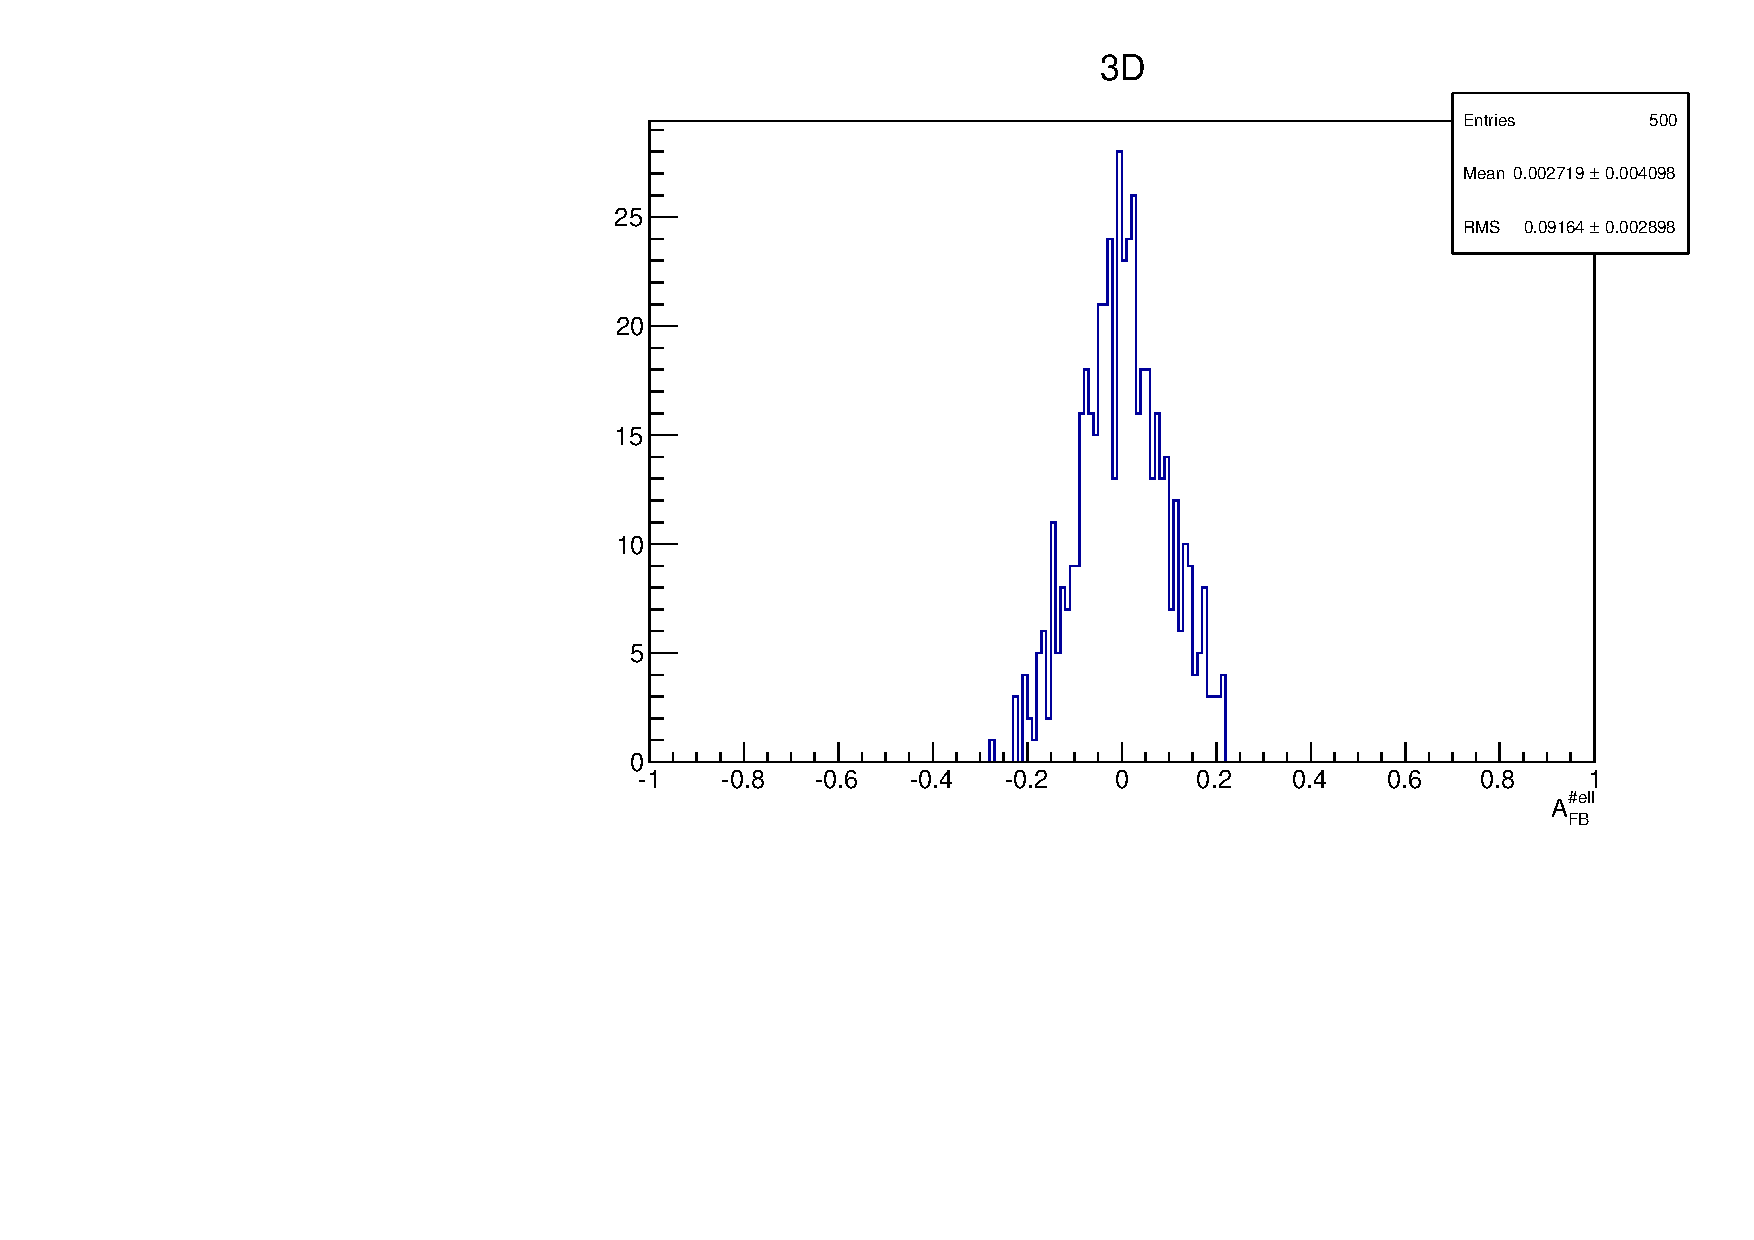
\includegraphics[width=0.3\textwidth]{Lmumu/figs/toys3D/B1/3D/toys3D_afb.pdf}
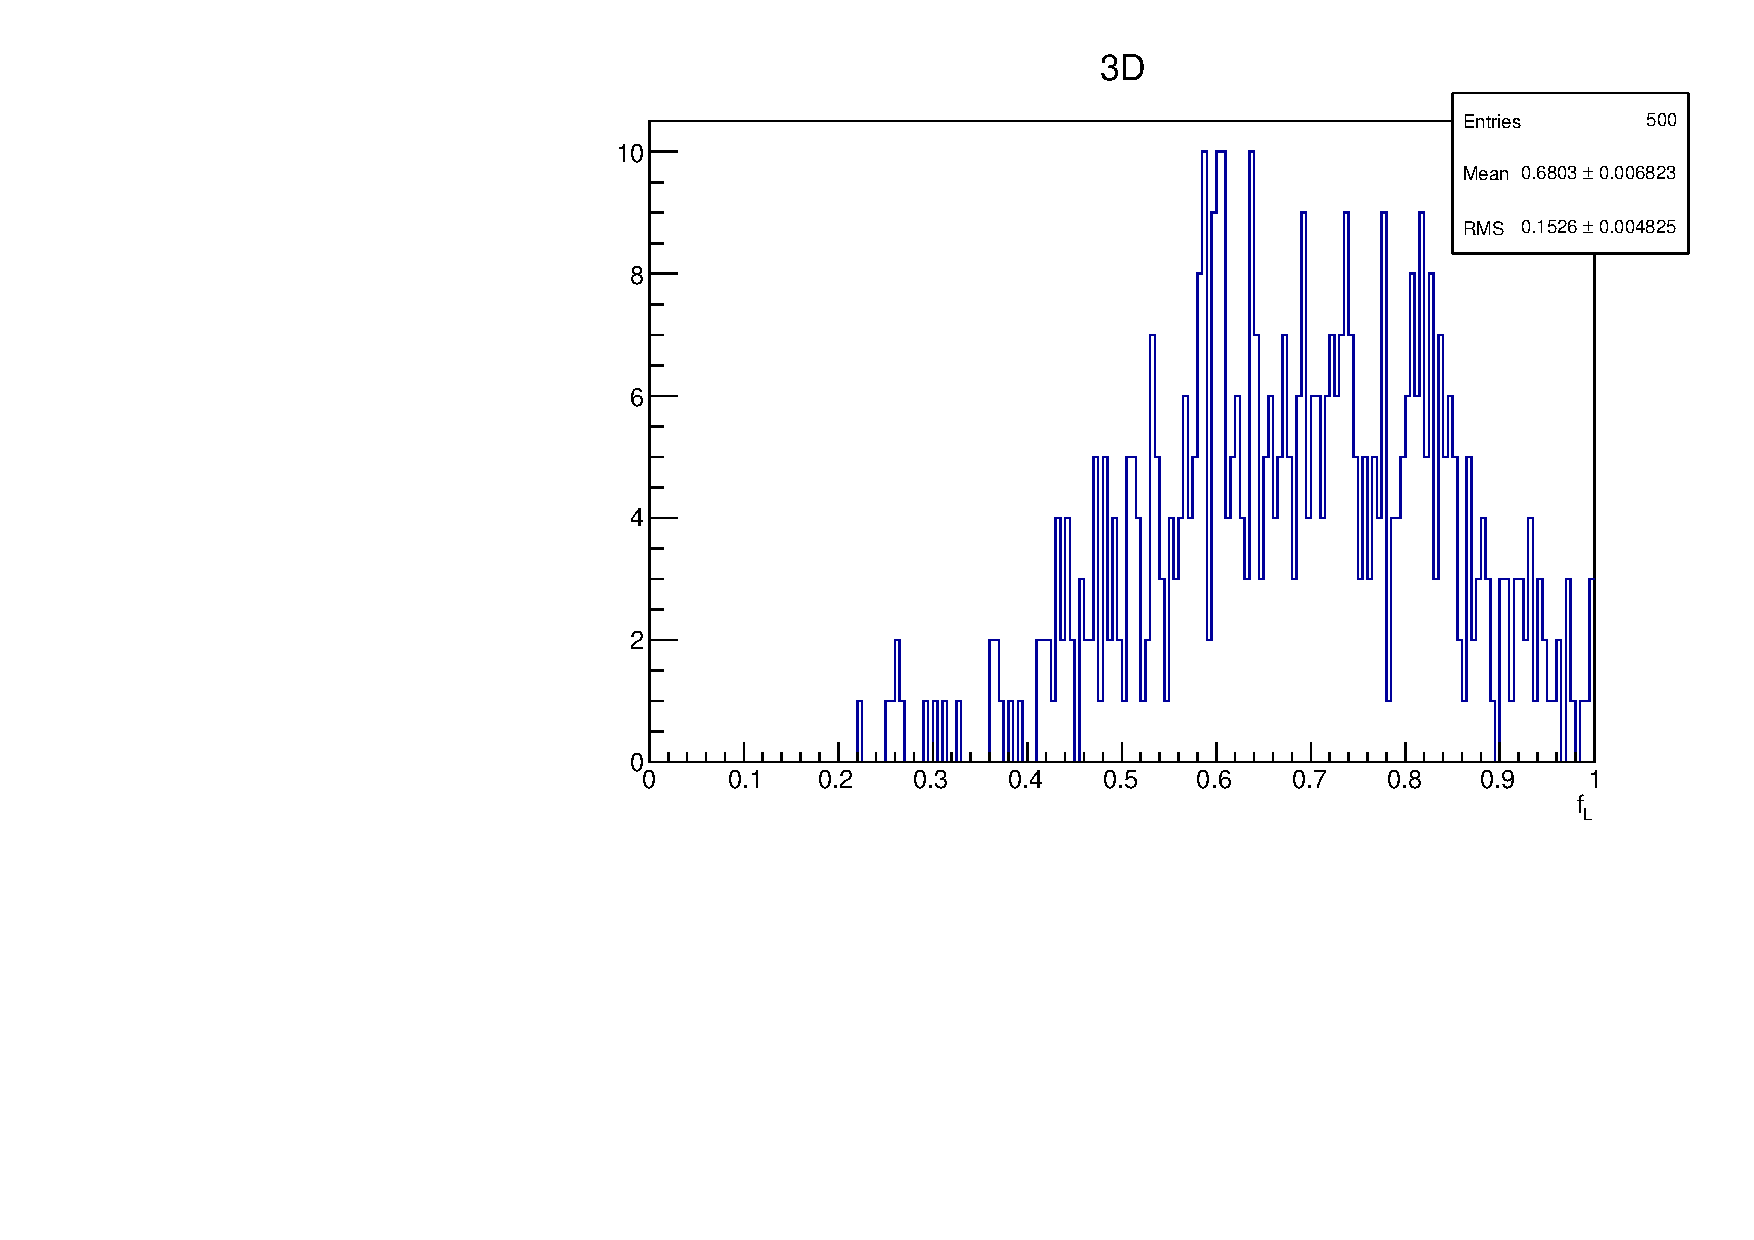
\includegraphics[width=0.3\textwidth]{Lmumu/figs/toys3D/B1/3D/toys3D_fL.pdf} \\
\caption{Distribution of oberved parameters of interest over 500 pseudo-experiments obtained
using the 1D fit method (top) and the 3D one (bottom). These toys correspond to events
generated with parameters and statistics corresponding to what is observed in the 15--20 \qsq nterval. }
\label{fig:3DtoyResults}
\end{figure}
%
\begin{figure}[h]
\centering
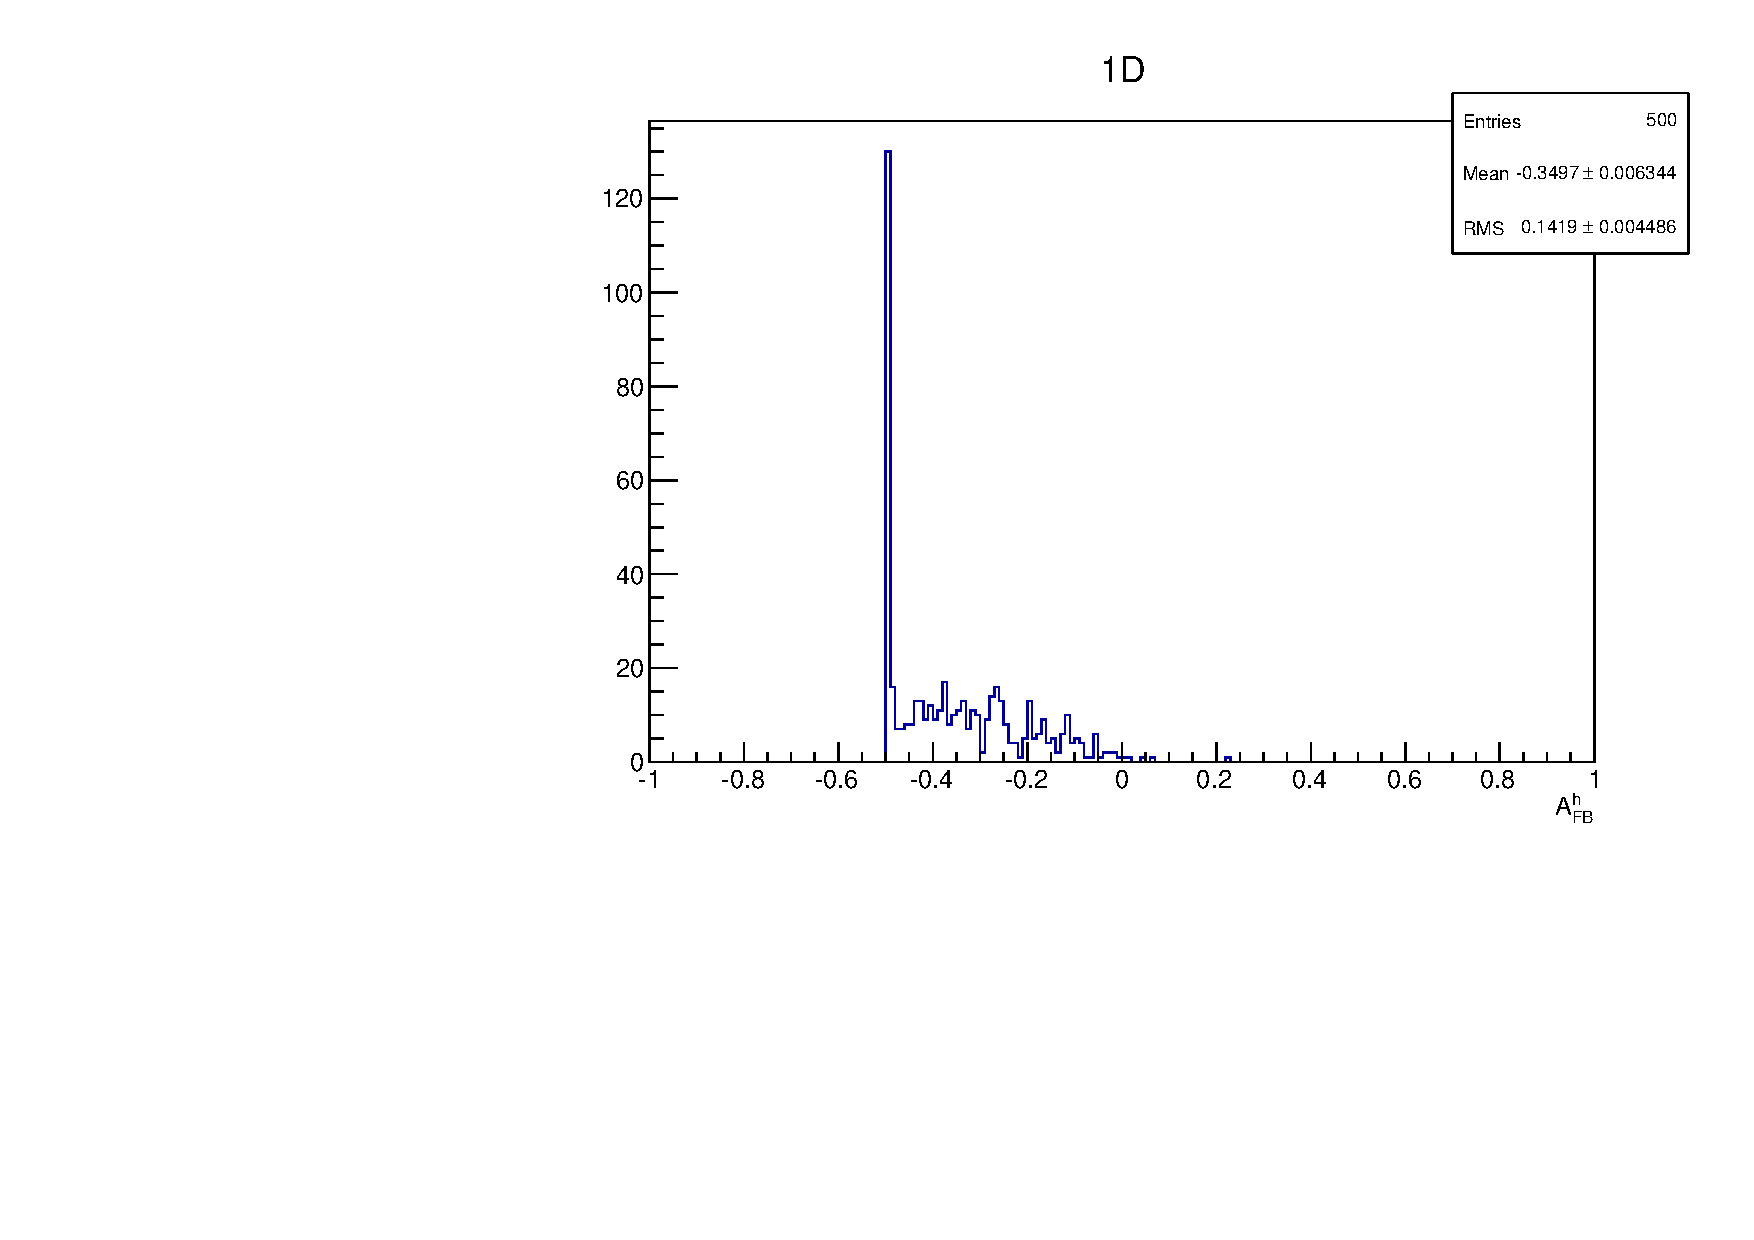
\includegraphics[width=0.3\textwidth]{Lmumu/figs/toys3D/B2/1D/toys3D_afbB.pdf}
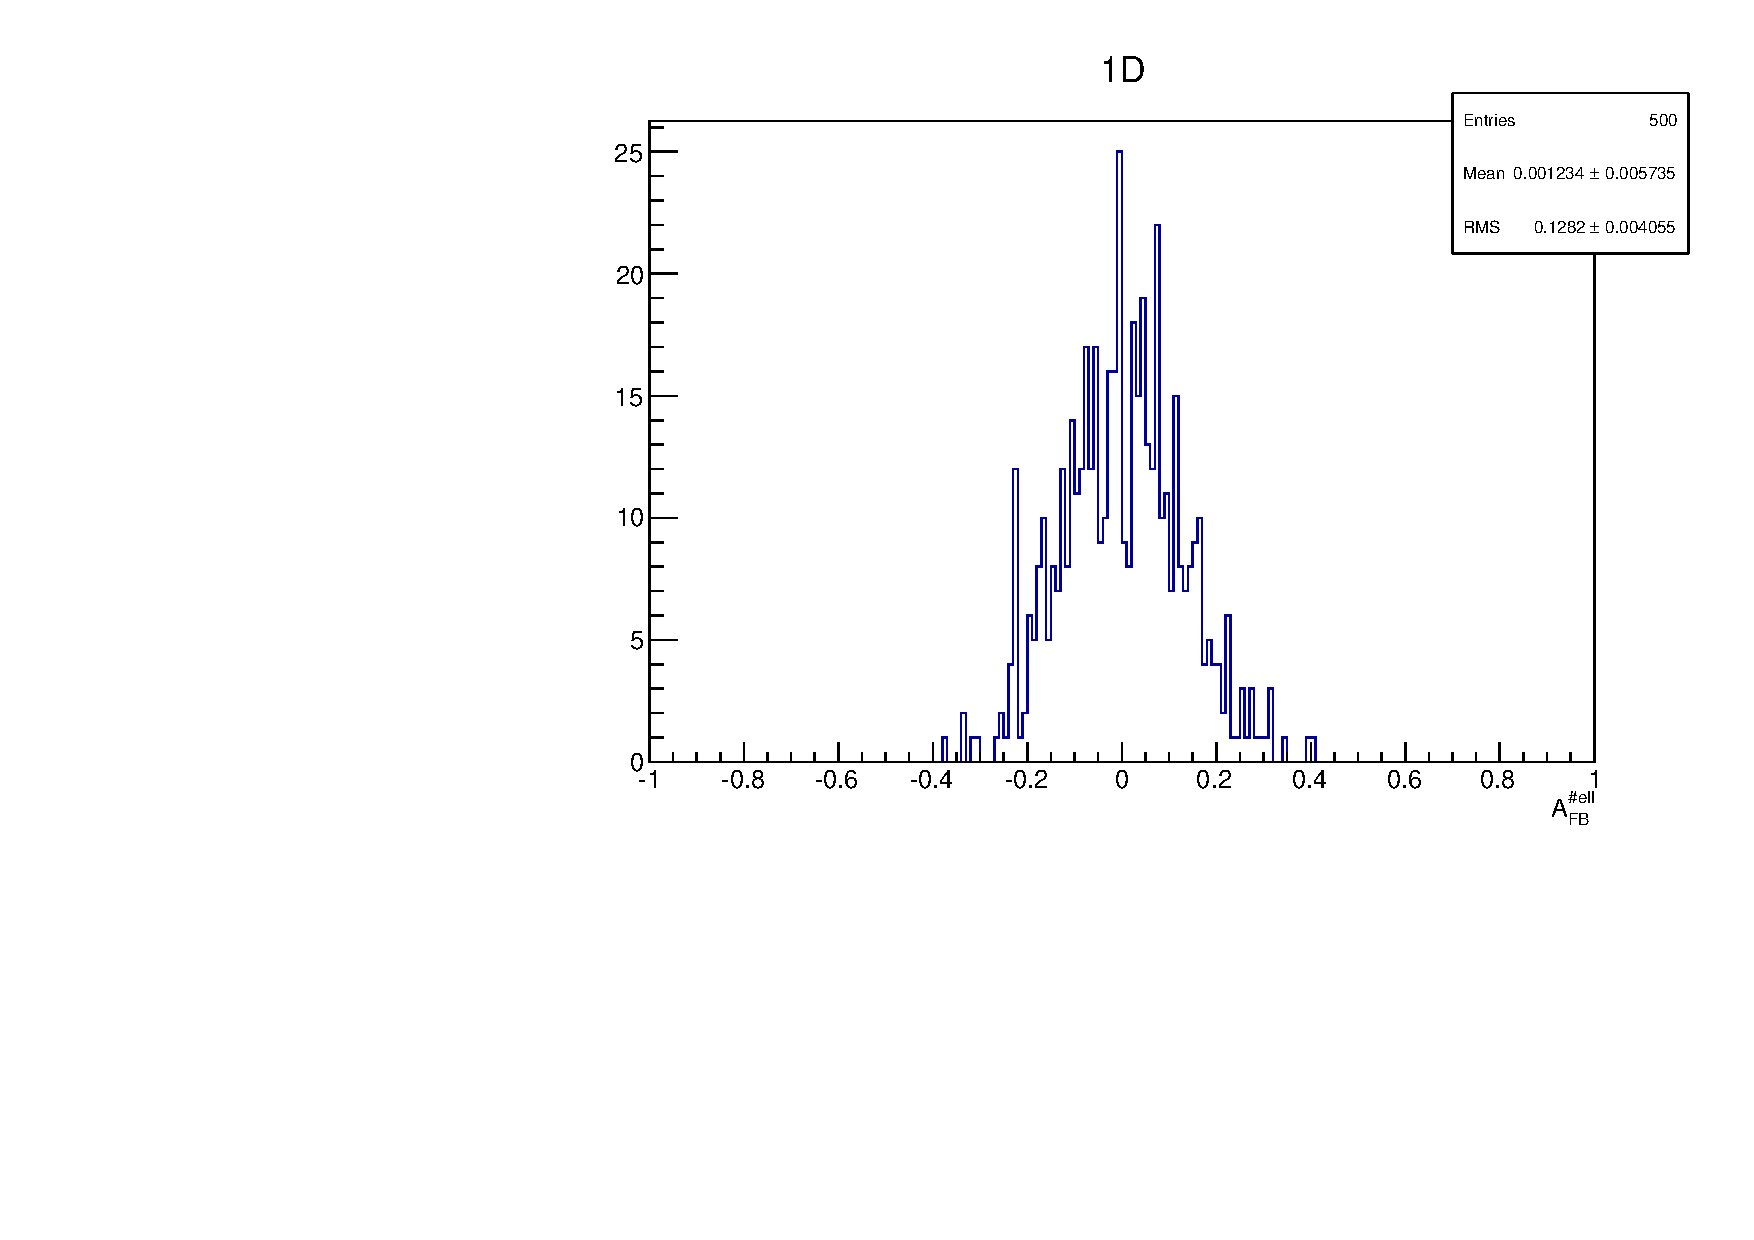
\includegraphics[width=0.3\textwidth]{Lmumu/figs/toys3D/B2/1D/toys3D_afb.pdf}
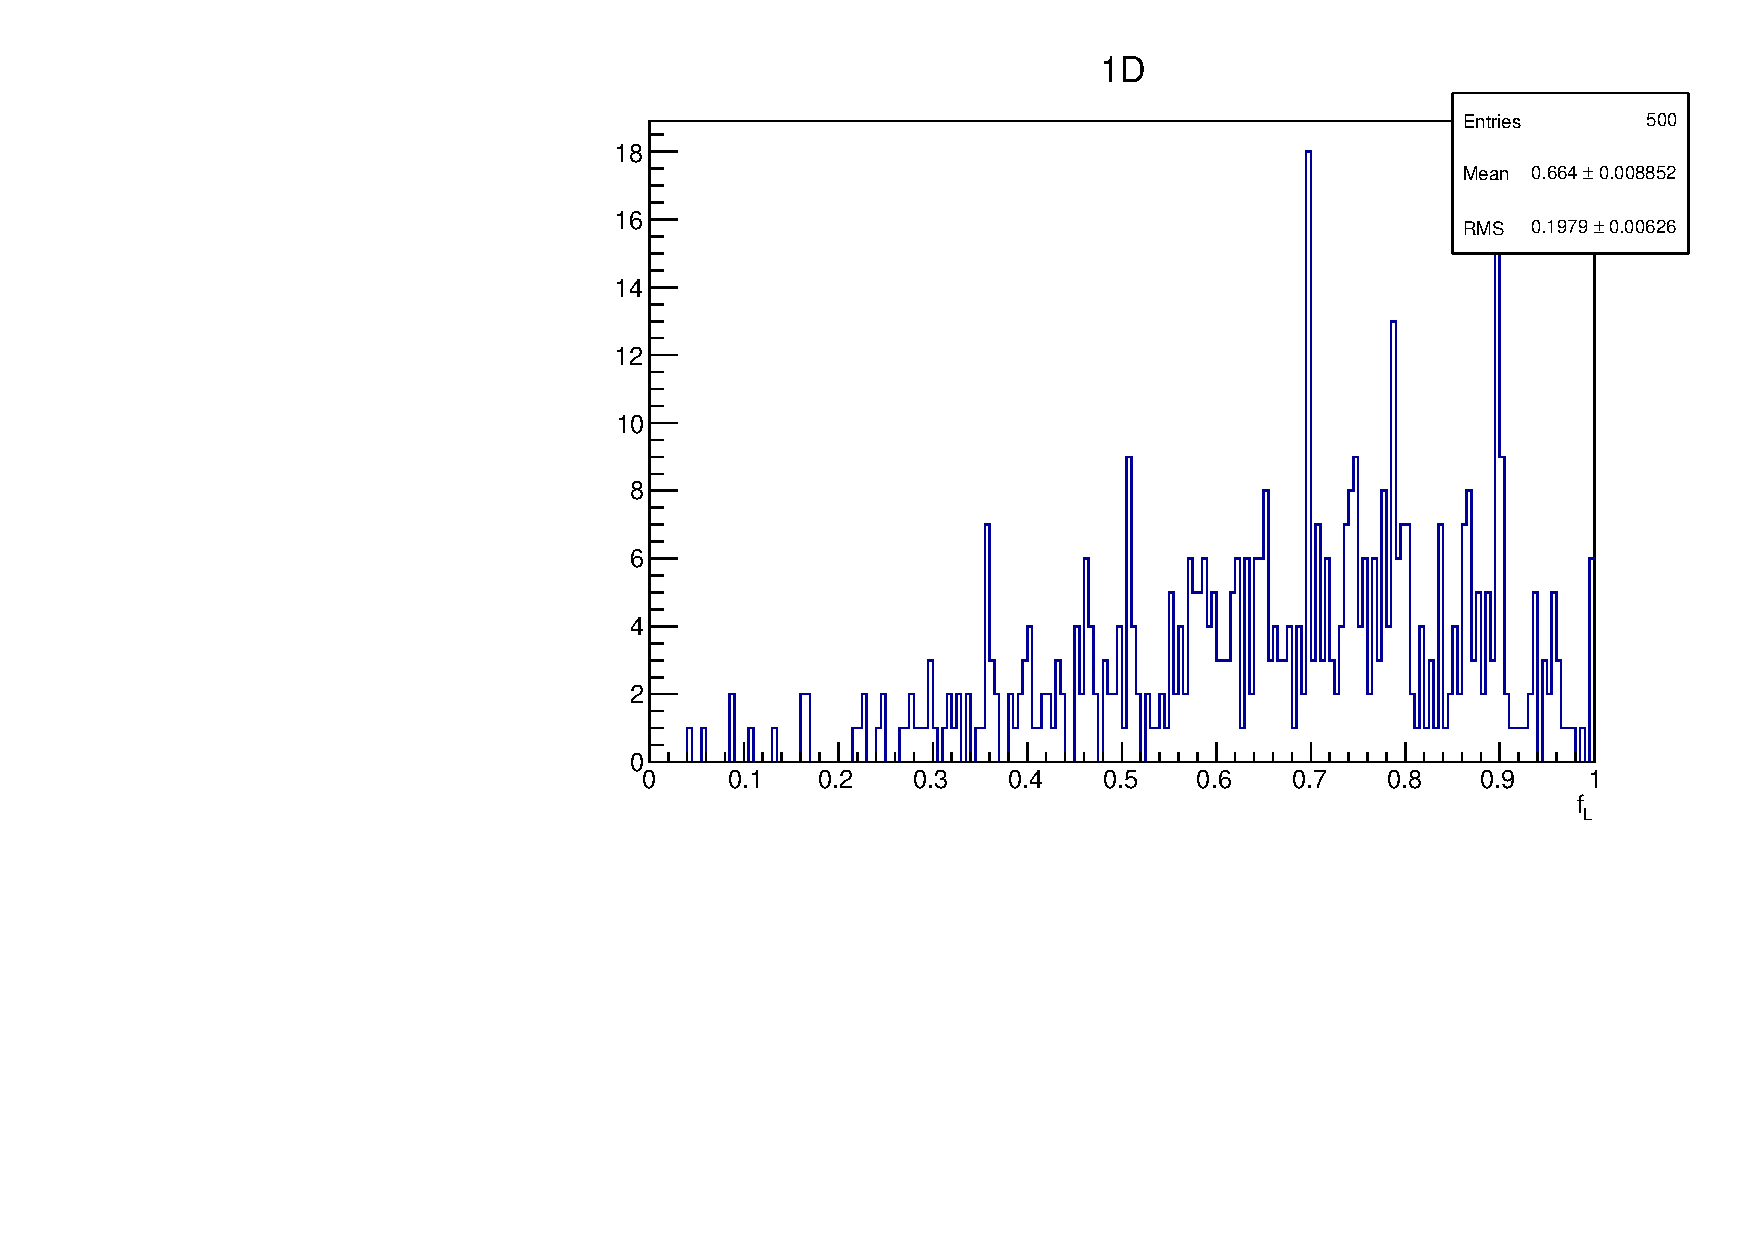
\includegraphics[width=0.3\textwidth]{Lmumu/figs/toys3D/B2/1D/toys3D_fL.pdf} \\
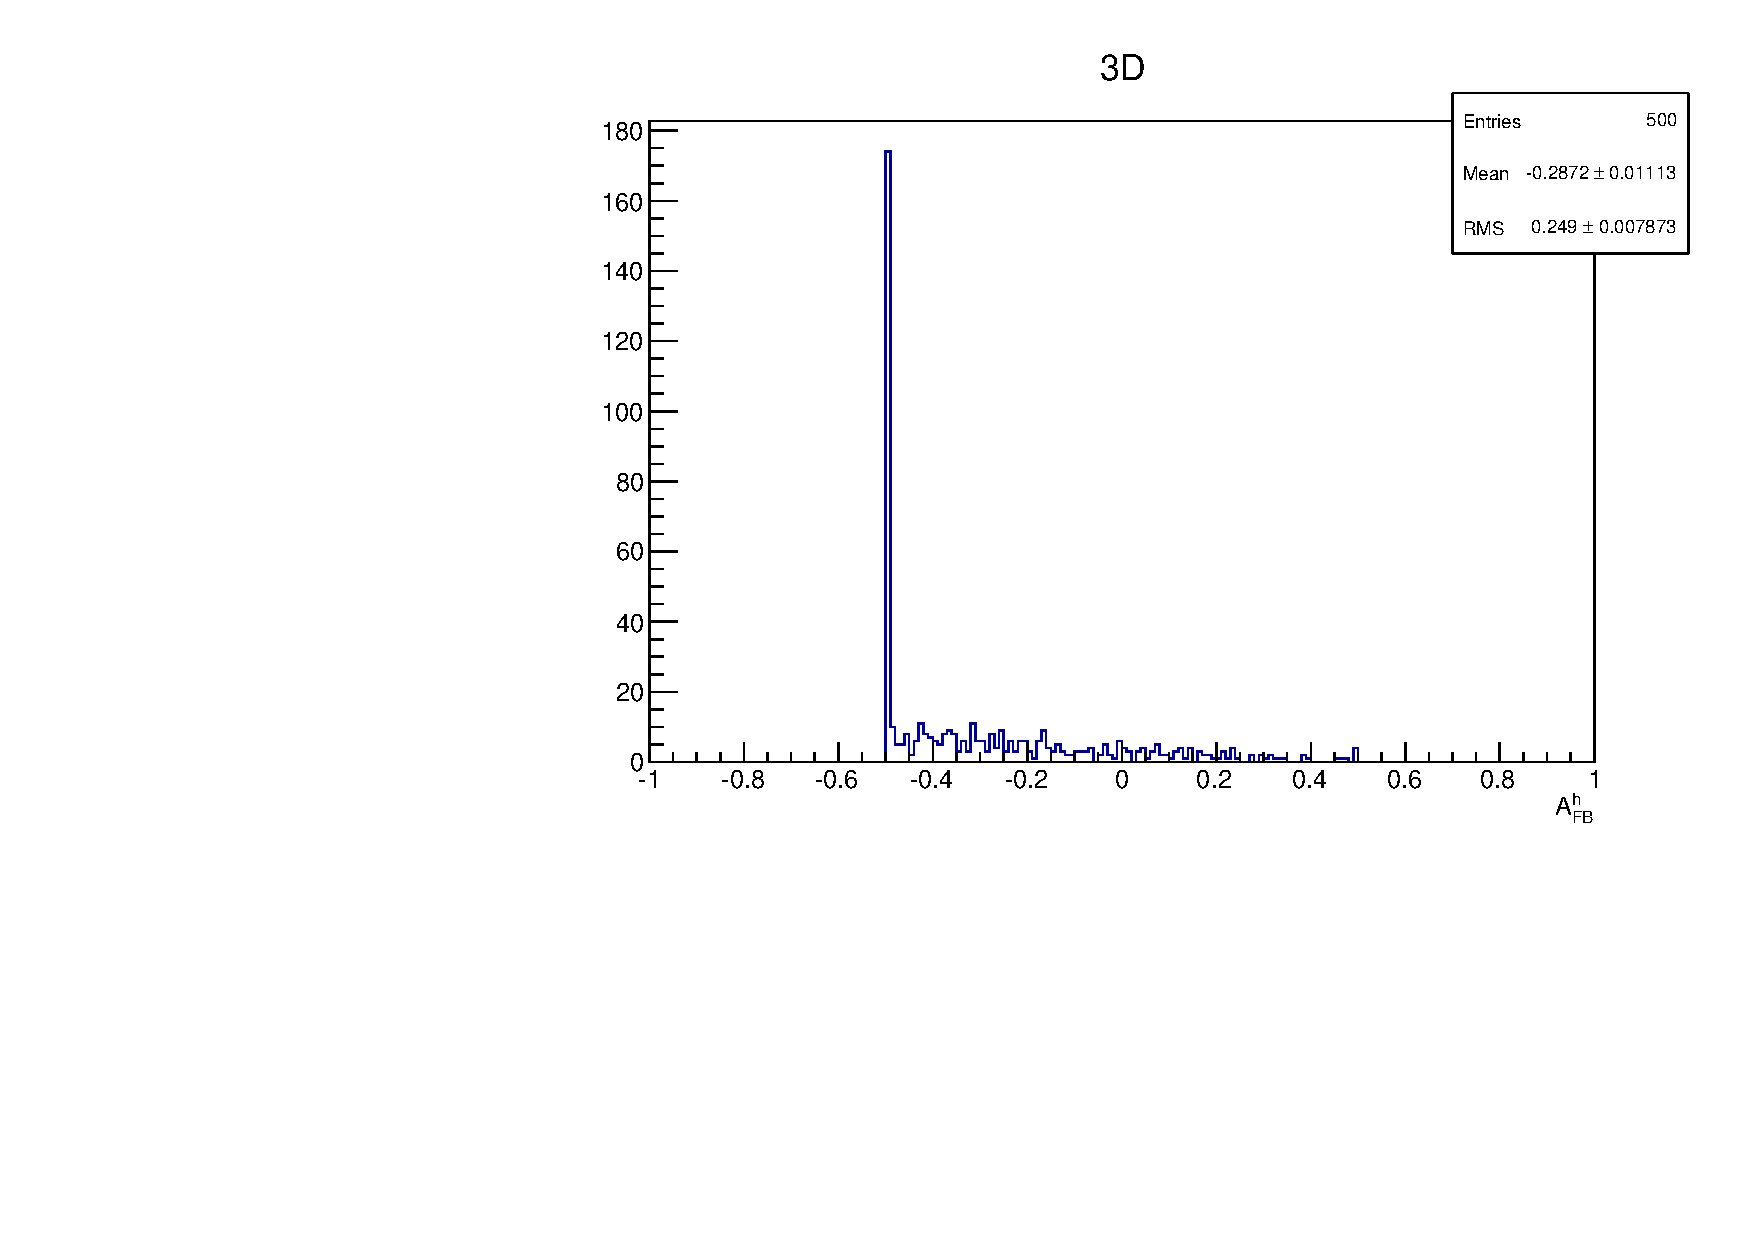
\includegraphics[width=0.3\textwidth]{Lmumu/figs/toys3D/B2/3D/toys3D_afbB.pdf}
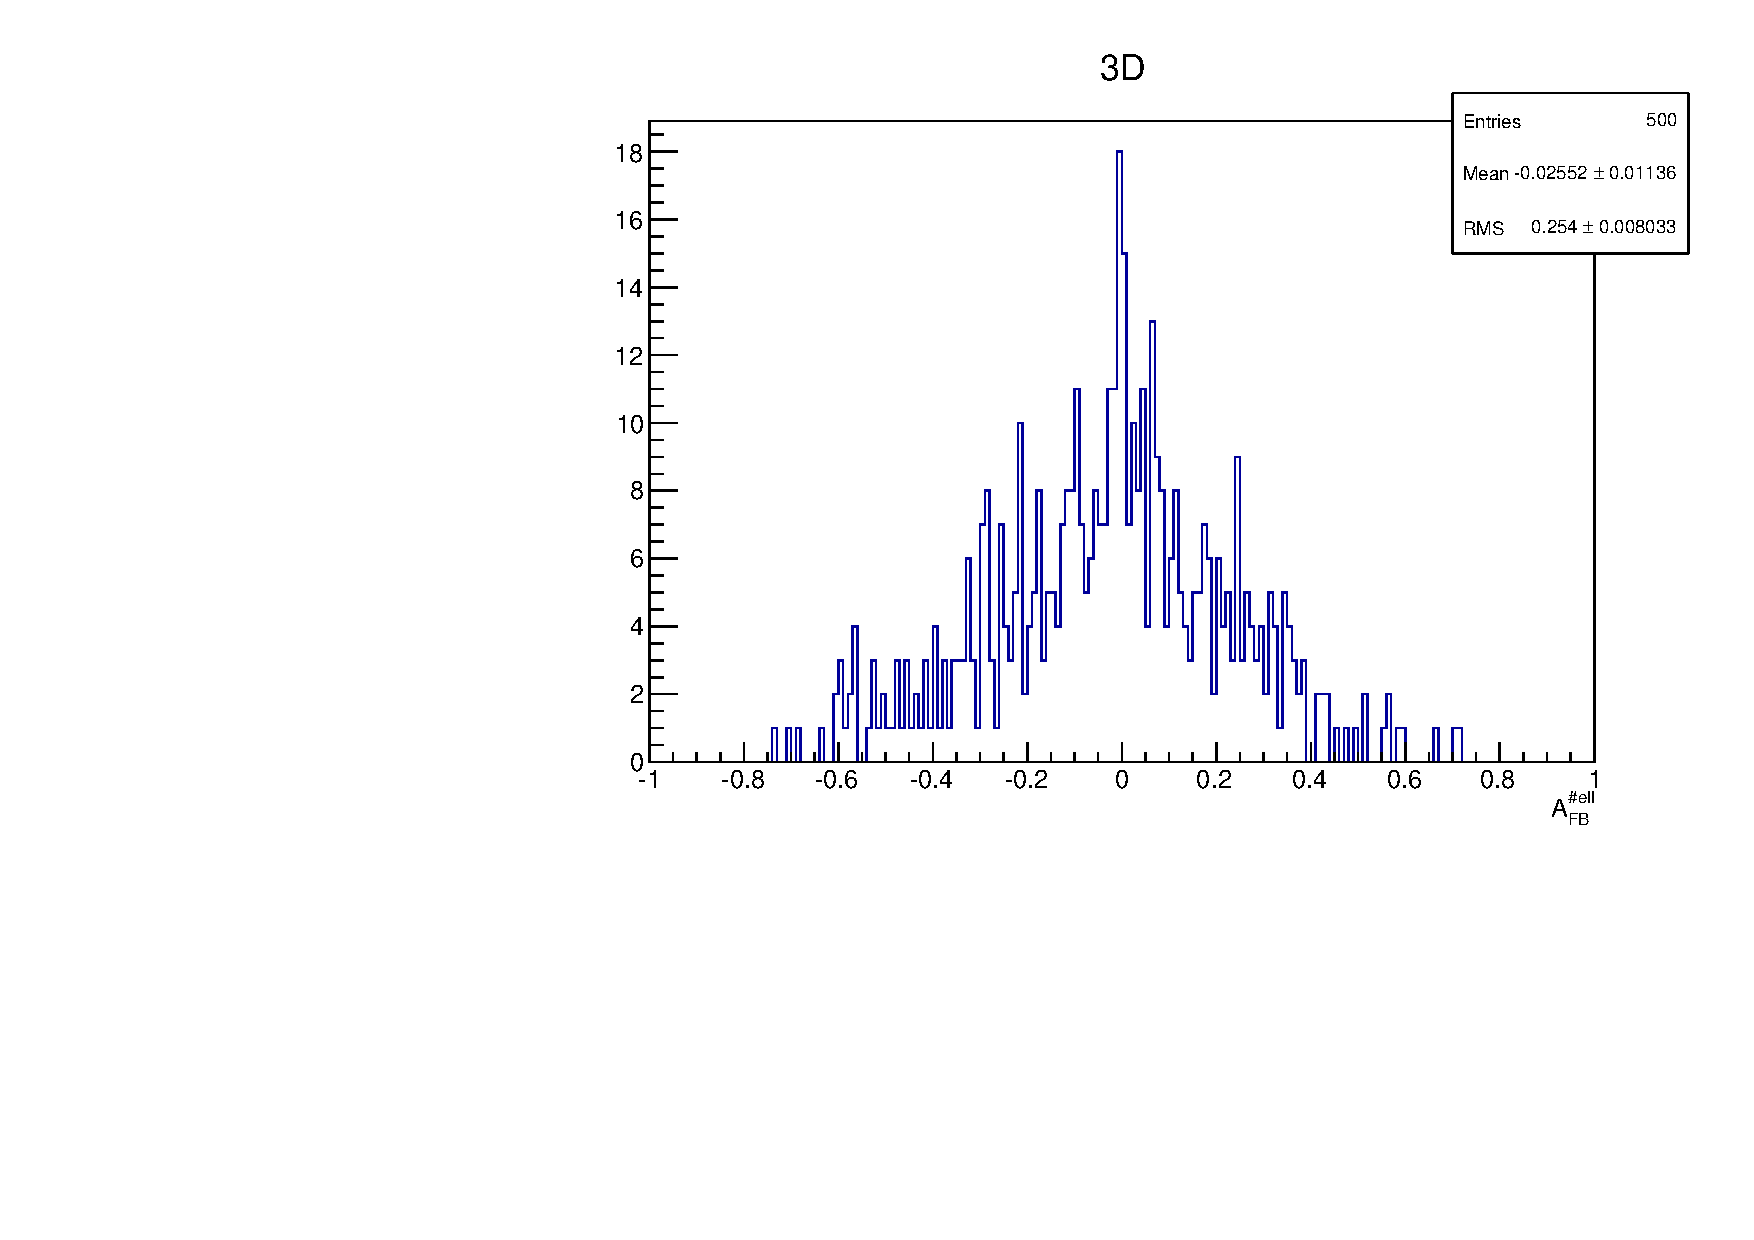
\includegraphics[width=0.3\textwidth]{Lmumu/figs/toys3D/B2/3D/toys3D_afb.pdf}
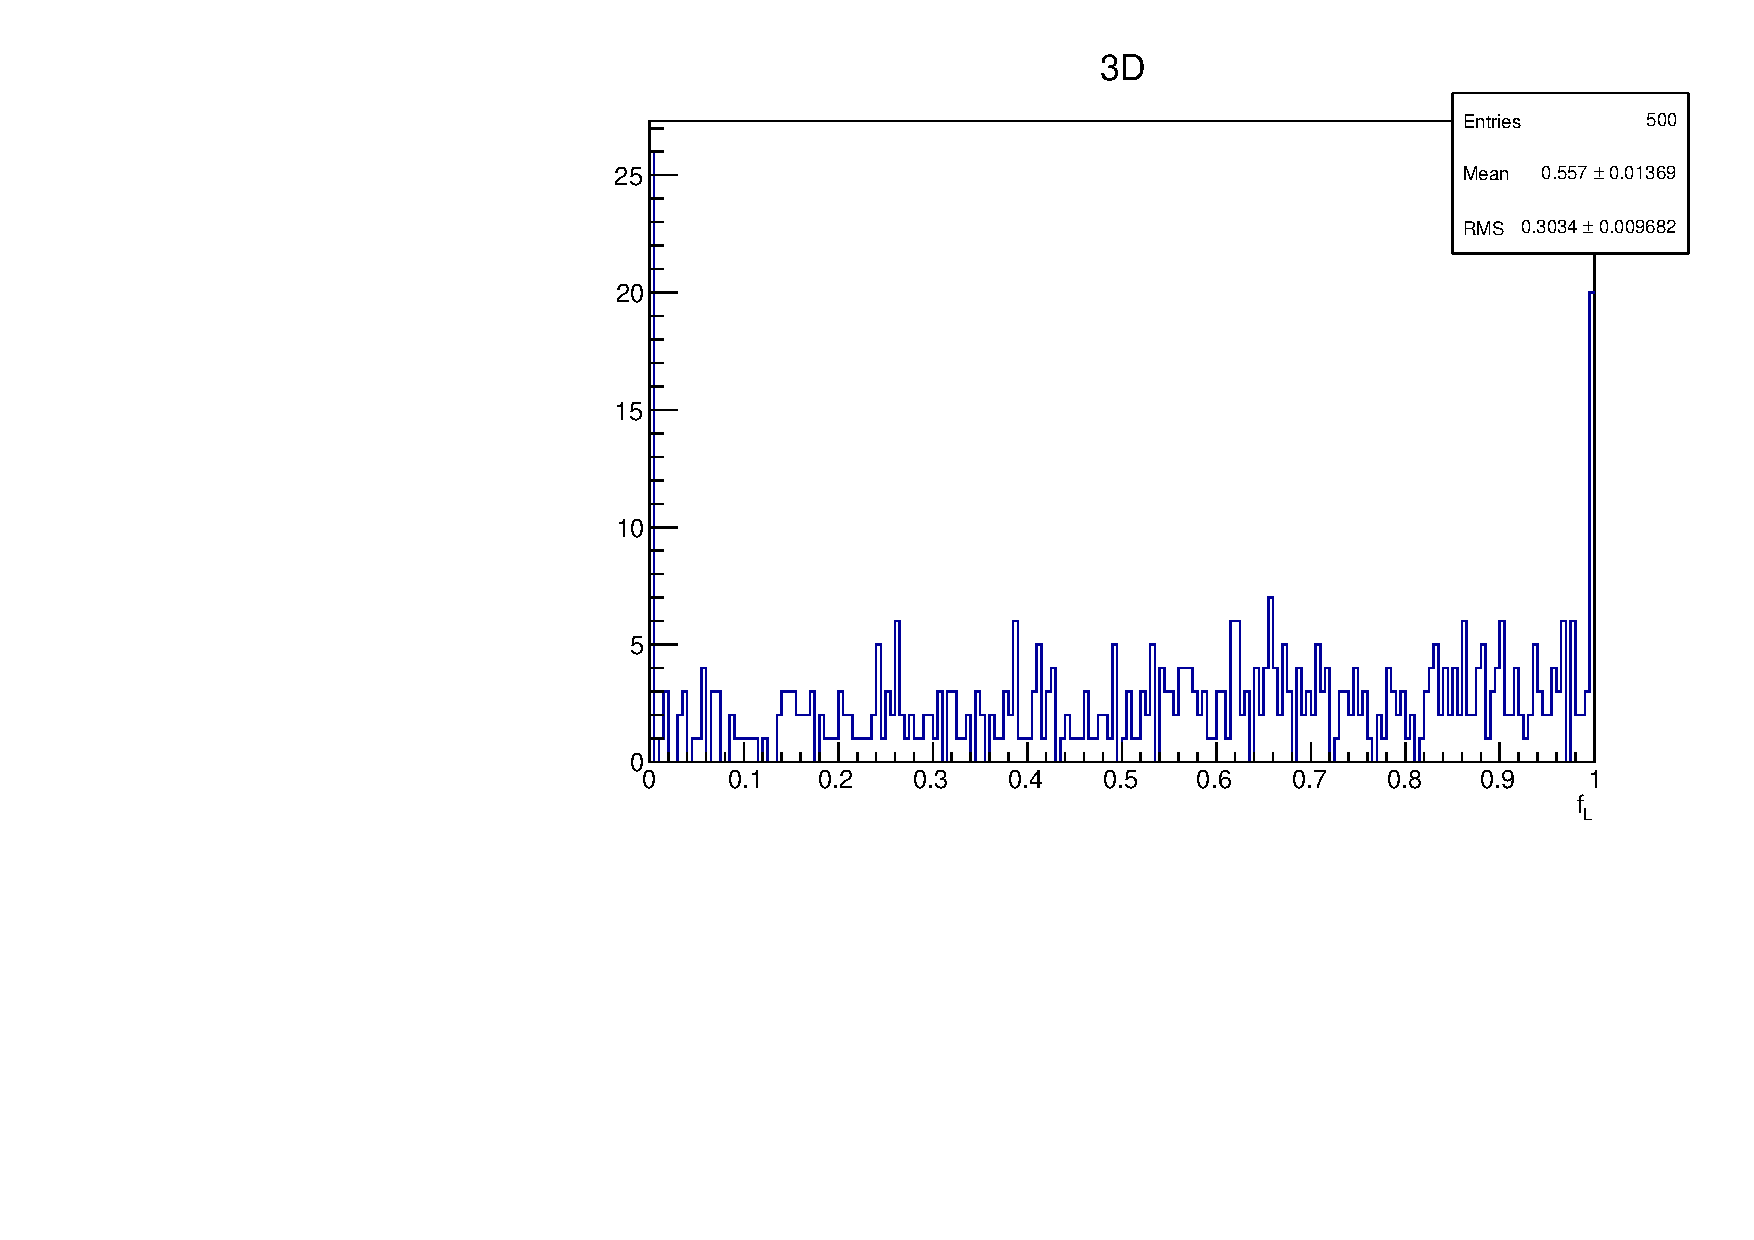
\includegraphics[width=0.3\textwidth]{Lmumu/figs/toys3D/B2/3D/toys3D_fL.pdf} \\
\caption{Distribution of oberved parameters of interest over 500 pseudo-experiments using the 1D fit
method (top) and the 3D one (bottom). These toys correspond to events generated with parameters
and statistics corresponding to what we observe in the 11--12.5 \qsq interval. }
\label{fig:3DtoyResults_lowest_stats}
\end{figure}
%
\begin{table}
\centering
\caption{RMS values for toy experiments on the extraction of the three parameters
of inetersts with the 1D or 3D fitting methods.}
\begin{tabular}{lcccc} \hline
\qsq bin                  &   Fit type 	 & $A_{FB}^h$  &  $A_{FB}^\ell$ &   $f_L$ 	 \\
\hline

\multirow{2}{*}{15.0-20.0} & 1D           &  0.070    &  0.055       &   0.099  \\
			    	       & 3D           &  0.092    &  0.095       &   0.153  \\
\hline
\multirow{2}{*}{11.0-12.5} & 1D           &  0.142    &  0.128       &   0.198  \\
					       & 3D           &  0.249    &  0.254       &   0.303  \\

\hline
\end{tabular}
\label{tab:3DtoyResults}
\end{table}

%In all cases we notice a slight bias in the fitting result. There fore we 
%assign as a systematic the full difference we observe on toys.
%Values of the systematic are reported in table \ref{tab:biassys} in bins of \qsq.

%\begin{table}
%\centering
%\begin{tabular}{lcccc} \hline\hline
%\qsq bin    &   $A_{FB}^\ell$			&  		 $f_L$ 	 			 &		 $A_{FB}^h$  		 \\
%\hline
%0.1-2.0		&	$-0.01126 \pm 0.01272$  &  $-0.14299 \pm 0.01551$    &  $0.04002 \pm 0.00950$    \\
%11.0-12.5	&	$0.00123 \pm 0.00574$	&  $-0.03601 \pm 0.00885$	 &  $0.02030 \pm 0.00634$  	\\
%15.0-16.0	&	$0.00592 \pm 0.00555$	&  $-0.03112 \pm 0.00880$	 &  $0.00772 \pm 0.00577$  	\\
%16.0-18.0	&	$0.00973 \pm 0.00389$	&  $0.00115 \pm 0.00634$	 &  $-0.00161 \pm 0.00428$  	\\
%18.0-20.0	&	$-0.00400 \pm 0.00391$	&  $-0.00306 \pm 0.00728$	 &  $0.00258 \pm 0.00458$  	\\
%\hline
%15.0-20.0	&	$-0.00052 \pm 0.00247$  &  $-0.00424 \pm 0.00441$     &  $-0.00100 \pm 0.00316$   \\
%\hline
%\end{tabular}
%\caption{Absolute values of systematic undertainties due to fit bias in bins of \qsq.}
%\label{tab:biassys}
%\end{table}



